\documentclass[a4paper,12pt]{article}

\usepackage{amsmath,amssymb,amsfonts,gensymb,mathtext,enumerate,float,cite}
\usepackage[T2A]{fontenc}
\usepackage[utf8]{inputenc}
\usepackage[english,russian]{babel}
\usepackage{indentfirst}
\usepackage[unicode=true]{hyperref}
\usepackage{multirow}
\usepackage{array}	
\usepackage[dvips]{graphicx}
\usepackage{xymtexpdf}
\usepackage{cmap}
\graphicspath{{images/}}



\usepackage{setspace}
% полуторный интервал
\onehalfspacing
\usepackage[14pt]{extsizes}

\hypersetup{
pdfborder={0 0 0},
pdfauthor={Lukianova Mariia Antonovna},
pdftitle={Diploma},
}

\usepackage{geometry}\geometry{left=3cm}
\geometry{right=2cm}
\geometry{top=2cm}
\geometry{bottom=2.5cm}

\numberwithin{equation}{section}
\numberwithin{figure}{section}
\numberwithin{table}{section}

\setcounter{tocdepth}{4}
\setcounter{secnumdepth}{4}



\RequirePackage{caption}
\DeclareCaptionLabelSeparator{defffis}{ -- }
\captionsetup{justification=centering,labelsep=defffis}
\usepackage{subfigure}
%\usepackage{subcaption}
\renewcommand{\thesubfigure}{(\asbuk{subfigure})}
\begin{document}
\righthyphenmin=20
\renewcommand{\figurename}{Рисунок}
\begin{titlepage}
\newpage

\begin{center}

\textbf{Московский государственный университет\\ имени М.В. Ломоносова}\\
\textbf{Химический факультет}\\
\text{Кафедра физической химии}\\
\text{Лаборатория строения конденсированных систем}
\end{center}
\vspace{1cm}


\vspace{8em}
\begin{center}
\textsc{\textbf{Хайбрахманов Артур Ильнурович}}
\vspace{1cm}


\textsc{\textbf{\large Применение методов ИИ для решения задач рентгенодифракционных исследований}}


\vspace{1em}

\textsc{Дипломная работа}
\end{center}
\vspace{7em}
\begin{flushright}
Научный руководитель:\\
к.\,х.\,н., с.\,н.\,с. Дмитриенко А.\,О.

д.\,х.\,н., доцент Лысенко К.\,С.

\end{flushright}

\vspace{\fill}

\begin{center}
Москва, 2025
\end{center}

\end{titlepage}

\setcounter{page}{2}
\renewcommand{\contentsname}{Оглавление}
\sloppy{
\tableofcontents

}
\newpage
\section*{Список использованных сокращений}
\addcontentsline{toc}{section}{Список использованных сокращений}
ВУФ --- вакуумный ультрафиолет

ИК --- инфракрасный

КР --- катион-радикал

ПАУ --- полициклические ароматические углеводороды

СТВ --- сверхтонкое взаимодействие

СТС --- сверхтонкая структура

УФ --- ультрафиолетовый

ЭПР --- электронный парамагнитный резонанс

Ng --- noble gas (обозначение атома благородного газа)
\newpage
\section*{Введение}
\addcontentsline{toc}{section}{Введение}
\sloppy{
Проблема молекулярной эволюции органического вещества в космическом пространстве находится в фокусе современного естествознания на протяжении нескольких десятилетий и привлекает постоянное внимание специалистов в области физики, химии и биологии. Один из наиболее широко обсуждаемых аспектов заявленной проблемы связан с механизмом образования полициклических ароматических углеводородов (ПАУ), обнаруженных в межзвёздных объектах различных типов.

В последние два десятилетия интерес к этой проблеме возрос в связи с успехами современной радиоастрономии и молекулярной астрофизики, позволившими надёжно зарегистрировать наличие достаточно большого числа относительно сложных молекул в различных космических объектах, а также планированием и осуществлением амбициозных космических миссий по исследованию дальнего космоса. Несмотря на очевидные успехи этих работ в последние годы, их выводы отчасти спекулятивны и нуждаются в экспериментальном и теоретическом обосновании.

Гипотеза об образовании ПАУ в межзвёздном пространстве была сформулирована на основе наблюдательных данных более 30 лет назад. С тех пор появилось большое число работ в этом направлении. Наличие ПАУ и других ароматических молекул (в основном, в ионизированном состоянии) в холодных межзвёздных средах не вызывает никаких сомнений, но в настоящее время остаётся открытым вопрос о механизмах, которые могут приводить к образованию столь сложных молекул ПАУ в межзвёздном пространстве.

Центральное место на пути построения сложных ароматических структур отводится бензолу, обнаруженному в диффузных молекулярных облаках. Реакции радикальных и ионных интермедиатов, возникающих из бензола (C$_6$H$_5^\bullet$, C$_6$H$_5^+$, C$_6$H$_7^+$), имеют ключевое значение для синтеза ПАУ во всех вариантах предложенных схем. Однако такие пути вовсе не очевидны с точки зрения традиционных представлений о фотохимии и радиационной химии бензола. Известно, что фотолиз бензола в конденсированных средах, в основном, приводит к образованию различных валентных изомеров, в которых не сохраняется ароматическое кольцо, а фенильных радикалов практически не образуется. Те же основные продукты, хотя и в другом соотношении, были обнаружены при УФ/ВУФ фотолизе матрично-изолированного бензола (в твёрдом пара-водороде наблюдался также радикал C$_6$H$_7^\bullet$ вследствие реакций атомов водорода из матрицы). Природа возбуждённых состояний, ответственных за реализацию различных каналов, остаётся дискуссионной, практически нет данных о реакциях высших триплетных состояний. С другой стороны, в радиационной химии имеется устойчивый стереотип о <<радиационной стойкости>> бензола на молекулярном уровне (очень низкий выход молекулярного водорода и фенильных радикалов). В действительности, однако, эти данные относятся не к молекулам бензола, а к жидкому или твёрдому бензолу, для которого характерна эффективная диссипация энергии вследствие образования эксимеров.

Данная работа посвящена моделированию важнейших элементарных стадий низкотемпературных радиационно-индуцированных процессов, приводящих в конечном итоге к образованию ПАУ. В качестве ключевой промежуточной структуры рассматривается молекула бензола – простейшая ароматическая молекула, обнаруженная в межзвёздном пространстве. Смысл использованного подхода состоит не в имитации условий и состава среды, а в направленном варьировании характеристик матриц (потенциал ионизации, поляризуемость, жёсткость) для моделирования каналов превращений, протекающих через различные ионные и возбуждённые состояния.

Такой подход позволяет, в принципе, установить общие закономерности ранних стадий радиационно-химических превращений органических молекул в жёстком окружении при криогенных температурах и сформулировать представления о механизмах влияния окружения на эти превращения, что имеет большое значение как для лабораторной астрохимии, так и для фундаментальной радиационной химии.

}
\newpage
\section{обзор}
\section{Обзор литературы}
\sloppy{
В данном обзоре проведён анализ имеющихся работ по изучению радиолиза и фотолиза бензола, изложены основы метода матричной изоляции и особенности радиолиза в этих условиях.

\subsection{Метод матричной изоляции}
\label{isolation}
Изучение строения и свойств высокореакционноспособных частиц, таких как, например, радикалы и ион-радикалы, представляет собой нетривиальную экспериментальную задачу.
Одним из подходов к её решению является применение метода матричной изоляции~--- замораживания молекул исследуемого вещества в жёстком окружении (матрице) химически инертного вещества.
Кроме того, применение данного метода позволяет изучать <<молекулярные>> свойства вещества, которые обусловлены только свойствами отдельной молекулы
и не связаны с взаимодействием с окружением в конденсированной фазе.
Для его реализации необходимо создать малую концентрацию исследуемого вещества и выбрать в качестве матрицы инертное в условиях эксперимента вещество.
Типичные для матричной изоляции разбавления составляют от 1:1000 до 1:10000 (иногда применяют разбавление 1:100). Уже при соотношении 1:1000 достигается изоляция почти 99\%
слабовзаимодействующих молекул \cite{MI}.

При выборе матричного вещества руководствуются следующими требованиями:
\begin{itemize}
\item химическая инертность по отношению к исследуемому веществу и продуктам его реакций;
\item жёсткость, препятствующая взаимодействию изолированных частиц;
\item низкая поляризуемость;
\item прозрачность в необходимом диапазоне электромагнитного спектра или отсутствие магнитных ядер (при применении ЭПР спектроскопии).
\end{itemize}

Перечисленным требованиям удовлетворяют матрицы твёрдых инертных газов (неон, аргон, криптон, ксенон) \cite{MI}. Неон обладает самой низкой поляризуемостью, меньше всего возмущает колебательную структуру изолированной частицы,
а значит лучше всего подходит для определения спектроскопических характеристик исследуемых веществ. Однако его применение сильно ограничено его малым температурным 
диапазоном стабильности (10--11~K).   Аргоновые матрицы наиболее распространены из-за малой поляризуемости и температурного 
диапазона стабильности до 38--40~K. Неон и аргон не имеют стабильных магнитных изотопов, что делает их привлекательными для изучения изолированных молекул методом ЭПР.
 Криптон и ксенон обладают большей поляризуемостью, однако такие матрицы устойчивы при более высоких температурах: до приблизительно 50~K и 80~K, соответственно.
 Криптон содержит 11,48\% магнитных ядер $^{83}$Kr, поэтому суперсверхтонкая структура в ЭПР-спектрах в данной матрице не разрешена. Ксенон содержит значительное
количество изотопов $^{129}$Xe и $^{131}$Xe, за счёт этого в спектрах ЭПР появляется дополнительная сложная подструктура, затрудняющая их интерпретацию. В некоторых случаях применяют матрицу $^{136}$Xe, не содержащую магнитных ядер, для 
получения хорошо разрешённых спектров ЭПР \cite{Feldman2012_}.
 Изменяя матричное вещество, можно моделировать различное взаимодействие изолированной молекулы с окружением и таким образом изучать влияние слабых взаимодействий, например, на процессы фотолиза и радиолиза.
 
В условиях матричной изоляции могут быть применены различные спектроскопические методы изучения структуры и свойств изолированных частиц. Одним из широко распространённых 
высокоинформативных методов является ИК-спектроскопия \cite{Feldman2014}.
 При интерпретации спектроскопических данных необходимо учитывать различные эффекты, обусловленные матрицей.
Так, в спектрах частиц, изолированных в матрице, полосы поглощения имеют гораздо меньшую ширину по сравнению
со спектрами в твёрдой, жидкой или газовой фазах за счёт отсутствия сильных межмолекулярных взаимодействий. Частым явлением является <<матричный сдвиг>> ---
изменение частоты максимума полосы поглощения частицы в матрице по сравнению со спектром в газовой фазе, возникающее за счёт возмущения матрицей колебательной структуры
частицы. В матрице неона эти сдвиги минимальны, тогда как в более поляризуемых матрицах (в особенности, в ксеноне) могут достигать значительных величин.
Встречается расщепление полос поглощения за счёт разных типов положения частицы в матрице (<<сайтов>>).  Для небольших молекул, способных вращаться в матрице, может 
наблюдаться вращательная подструктура. 

Для генерации активных частиц при использовании матричной изоляции используют различные методы. Существует два основных подхода: генерация активных частиц в 
газовой фазе с последующим осаждением их вместе с матрицей и генерация непосредственно в осаждённой матрице. Для первого подхода применяют высокотемпературное испарение,
лазерную абляцию,
пиролиз,
газовый разряд,
фотолиз и радиолиз в газовой фазе. Для второго~--- фотолиз и радиолиз в матрице \cite{MI}.
Последние указанные два метода принципиально отличаются по механизму взаимодействия с веществом.
При фотолизе в матрице излучение поглощается селективно молекулами исследуемого вещества, матрица служит резервуаром для рассеивания энергии и стабилизирующей средой для продуктов, благодаря этому начальные этапы фотолиза в условиях матричной изоляции похожи на таковые в газовой фазе.  
В случае радиолиза основная часть энергии поглощается матрицей. Эффективность радиационно-индуцированного разложения вещества в матрице зависит от эффективности передачи энергии с матрицы на молекулы исследуемого вещества. Типичные значения радиационно-химических выходов разложения молекул в матрицах составляют несколько единиц на 100 эВ. Приведём несколько значений радиационно-химических выходов 
разложения различных веществ в матрице аргона: HCN~--- 3.8~молек./100~эВ, ацетонитрил~--- 5~молек./100~эВ \cite{Kameneve_diss}, бутан~--- 2.9~молек./100~эВ, гептан~--- 1.8~молек./100~эВ \cite{Feldman1999_}. Типичные процессы, происходящие при радиолизе органических веществ в условиях матричной изоляции представлены уравнениями \ref{eq1}--\ref{eq7} (где Ng~--- атом благородного газа, M~--- молекула изолированного вещества, P~--- продукты радиолиза) \cite{Feldman2014, Feldman1999_, Feldman1997}. 

\begin{equation}\label{eq1}
\mathrm{ 
Ng \leadsto Ng^{+\bullet}, e^-, Ng^*}
\end{equation}
\begin{equation}\label{eq2}
\mathrm{
Ng^{+\bullet} + M \to (M^{+\bullet})^* + Ng}
\end{equation}
\begin{equation}\label{eq3}
\mathrm{
Ng^* + M \to M^* + Ng}
\end{equation}
\begin{equation}\label{eq4}
\mathrm{
(M^{+\bullet})^* \to M^{+\bullet}}
\end{equation}
\begin{equation}\label{eq5}
\mathrm{
(M^{+\bullet})^* \to P}
\end{equation}
\begin{equation}\label{eq6}
\mathrm{
M^{+\bullet} + e^- \to M^{**}}
\end{equation}
\begin{equation}\label{eq7}
\mathrm{
M^* \;(M^{**})\to P}
\end{equation}

При взаимодействии излучения с матрицей образуются катион-радикалы матричных атомов, экситоны и электроны (уравнение~\ref{eq1}).
Затем происходит передача заряда и возбуждения с матрицы на молекулы изолированного вещества (уравнения~\ref{eq2}, \ref{eq3}). При передаче <<дырки>> с матрицы на изолированную молекулу образуется катион-радикал в возбуждённом состоянии из-за разности потенциалов ионизации атомов матрицы и молекул рассматриваемого вещества. Это  верно для многих органических веществ (часто потенциал ионизации около 10~эВ), так как инертные газы имеют высокие потенциалы ионизации (21.56~эВ для Ne, 15.75~эВ для Ar, 14.0~эВ для Kr, 12.13~эВ для Xe \cite{xray}). Полученный возбуждённый КР может релаксировать в основное состояние (уравнение~\ref{eq4}) или приводить к образованию продуктов (уравнение~\ref{eq5}). Кроме того, КР может рекомбинировать с электронами с образованием возбуждённой молекулы (уравнение~\ref{eq6}).  Из возбуждённых состояний, в свою очередь, могут образовываться продукты
(уравнение~\ref{eq7}). 

Катион-радикалы, образующиеся при передаче энергии с матрицы на изолированную молекулу, обладают избыточной энергией, близкой к разности потенциалов ионизации. Потому в матрицах с более высокими потенциалами ионизации КР могут не стабилизироваться, а сразу же претерпевать фрагментацию. При этом КР некоторых алканов могут быть стабилизированы в матрице ксенона \cite{Feldman1999_}. Однако поляризуемость матрицы влияет на стабилизацию КР противоположным образом. КР могут депротонироваться при наличии акцептора протонов. Способность принимать протон для инертных газов коррелирует с поляризуемостью, то есть увеличивается от неона к ксенону \cite{NIST}. В матрицах аргона, криптона и ксенона зафиксированы стабилизированные протоны типа Ng$_2$H$^+$, возникающие, по-видимому, в результате реакции \ref{eq8} \cite{Bondybey1972, Kunttu1992}. Благодаря этой реакции, КР, обладающие значительной кислотностью (вода, метанол и др.) стабилизируются только в матрице неона \cite{Knight1992, Knight1995}.

\begin{equation}\label{eq8}
\mathrm{
H^+ + 2Ng \to Ng_2H^+}
\end{equation}

 Соединения типа Ng$_2$H$^+$ имеют характерные полосы в ИК-спектрах:  903.3 и 1139.6~см$^{-1}$ для Ar$_2$H$^+$ \cite{Bondybey1972};  852.5, 1007.7 и 1160.4~см$^{-1}$ для Kr$_2$H$^+$ \cite{Bondybey1972};  730.6, 842.7 и 953.4~см$^{-1}$ для Xe$_2$H$^+$ \cite{Kunttu1992}. Аналогичные соединения образуются в случае стабилизации дейтрона. В ИК-спектре их можно наблюдать по полосам поглощения при 644~см$^{-1}$ для Ar$_2$H$^+$ \cite{Bondybey1972}; 606~см$^{-1}$ для  Kr$_2$D$^+$ \cite{Bondybey1972}; 516.7~см$^{-1}$ для  Xe$_2$D$^+$ \cite{Kunttu1992}. Соединения типа Ng$_2$H$^+$ неустойчивы и даже при температуре 7~K гибнут со временем в темноте, а также при фотолизе видимым светом \cite{Bondybey1972}.


\subsection{Радиолиз бензола}
\label{radiolysis}
Радиолизу бензола посвящено множество работ. Многие из них направлены на установление конечных продуктов разложения бензола, но не на установление 
детального механизма. Кроме анализа этих работ, в данном разделе приведены имеющиеся данные о промежуточных частицах, образующихся при радиолизе бензола.
\subsubsection{Конечные продукты радиолиза бензола}
\label{products}
Большое количество работ, направленных на идентификацию конечных продуктов радиолиза бензола, было опубликовано в 1960--1980~гг. 

Радиолиз бензола
в газовой фазе изучен слабо. Существует всего несколько работ, в которых рассмотрен этот процесс. 
Так, показано, что при радиолизе бензола в газообразном состоянии радиационно-химический выход разложения составляет 
4--6~молекул/100~эВ \cite{burns1969, walzbach1968}. В работе \cite{burns1969} исследовали радиолиз бензола при температурах 260--390$^\circ$С. 
При помощи газовой хроматографии наблюдали образование водорода, метана, ацетилена, этана, этилена, бифенила и полимерных продуктов. Были установлены зависимости радиационно-химических выходов перечисленных продуктов
от плотности и температуры (для всех продуктов, кроме ацетилена, выходы увеличиваются с ростом температуры и уменьшаются с увеличением плотности). Сильнее всего с ростом температуры менялся выход водорода (от 0.1 до 3~молекул/100~эВ).
Авторы полагают, что при повышении плотности выход разложения бензола снижался из-за конкуренции между дезактивацией возбуждённых состояний и их превращением в продукты.

При радиолизе бензола в конденсированном состоянии наблюдаются низкие радиационно-химические выходы газообразных продуктов. Так, при облучении $\gamma$-лучами или электронами
 жидкого бензола выход водорода составляет около 0.04~молекул/100~эВ, выход ацетилена~--- 0.02~молекул/100~эВ \cite{Chapiro1977, Cherniak1964}. 
 При радиолизе твёрдого бензола при 160~K радиационно-химические выходы ещё ниже: $G$(H$_2$)~=~0.0085~молекул/100~эВ,  $G$(CH$_4$)~=~0.008~молекул/100~эВ, $G$(C$_2$H$_2$)~=~0.0016~молекул/100~эВ \cite{Solid}.

 При радиолизе жидкого дейтерированного бензола образуется молекулярный дейтерий, его радиационно-химический выход меньше, чем выход молекулярного водорода 
(0.017~молекул/100~эВ). 
Выход дейтерированного ацетилена не сильно отличается от его недейтерированного аналога (0.0133~молекул/100~эВ). При радиолизе смеси C$_6$H$_6$--C$_6$D$_6$
(1:1) образуется водород с соотношением изотопологов H$_2$:HD:D$_2 = 52.1:33.1:14.8$ \cite{Gordon1952}.
 
 Выход тяжёлых продуктов при радиолизе бензола на несколько порядков выше. Основным продуктом является так называемый 
 <<полимер>> --- смесь веществ, полученных объединением нескольких молекул бензола. Радиационно-химический выход превращения бензола в <<полимер>> составляет 0.75~молекул/100~эВ \cite{Patrick1954}. 
 Отношение содержания углерода и водорода варьируется в <<полимере>> от 1.0 до 1.6, 
 средняя молекулярная масса растёт с поглощённой дозой и  может достигать 430~г/моль при дозе около 10$^7$~Гр \cite{Patrick1954}. 
 При помощи хроматографии показано, что при радиолизе жидкого бензола образуются бифенил, циклогексадиены, фенилциклогексадиены, бициклогексадиены, а так же различные терфенилы \cite{Cherniak1964, Zimmerli1969}.
 
В работе группы Страццуллы \cite{Strazzulla1991} чистый замороженный бензол облучали ионами гелия с энергией 3 кэВ.
По ИК-спектру облучённых образцов сделаны предположения о составе продуктов радиолиза. Широкие полосы молекулярной матрицы не дали возможности для точного отнесения.
Однако авторы называют одними из основных продуктов ацетилен и монозамещённый ацетилен, кроме того наблюдают полосы, относимые к С=С и C--H колебаниям в замещённом бензольном кольце, C--H колебаниям в алифатических фрагментах.
Сделано предположение о существовании продукта со структурой HC$\equiv$C\nobreakdash--CH$_2$\nobreakdash--C$\equiv$C\nobreakdash--C$_6$H$_5$.

 Р. Х. Шулер и Дж. А. ЛаВерне проводили систематические исследования радиолиза бензола тяжёлыми ионами. 
Изучен радиационно-химический выход водорода при бомбардировке протонами, дейтронами, ионами гелия \cite{Schuler1965},  $^7$Li \cite{LaVerne1982}, $^9$Be, $^{11}$B, $^{12}$C \cite{LaVerne1984}.
Установлено, что даже при малых энергиях тяжёлых частиц выход водорода значительно превышает выход при облучении электронами или $\gamma$-лучами.
Показан резкий рост радиационно-химического выхода водорода при увеличении ЛПЭ.

В работе \cite{LaVerne2002} проведено сравнение радиолиза жидкого бензола $\gamma$\nobreakdash-лучами и тяжёлыми ионами. При помощи газовой хроматографии с масс-спектрометрическим детектированием были определены выходы продуктов. Показано, что несмотря на то, что
 при $\gamma$\nobreakdash-радиолизе почти все возбуждённые состояния релаксируют до основного электронного состояния, при облучении тяжёлыми ионами реакции возбуждённых состояний приводят к значительным выходам продуктов.
 Основными зафиксированными продуктами названы бифенил, молекулярный водород и фенильный радикал. Последний регистрировали в экспериментах с добавками иода (по образованию иодбензола). 
  Показано, что фенильный радикал может образовывать с бензолом относительно долгоживущий аддукт, который затем ведёт к образованию <<полимеров>>.
 Выход бифенила не зависел от типа облучения и составлял 0.075~молекул/100~эВ. Кроме того, на основании сходства зависимостей флюоресценции и выхода H$_2$ от ЛПЭ авторы делают вывод о том, что предшественником молекулярного водорода является
 синглетное возбуждённое состояние.

 В 2005 году опубликована работа \cite{Ruiterkamp2005}, в которой было проведено сравнение УФ-фотолиза и бомбардировки протонами бензола. Кроме облучения чистого бензола 
были проведены исследования поведения молекул бензола, изолированных в матрице твёрдого аргона, а также в модельных кислородсодержащих астрохимических льдах.
Идентификацию продуктов и оценку эффективности разложения бензола проводили при помощи ИК-спектроскопии. Точное определение продуктов радиолиза и фотолиза не было основной целью работы,
однако авторы полагают, что основными продуктами в случае матрично-изолированного бензола являются продукты распада: ацетилен и метилацетилен. 
Кроме того, часть полос поглощения авторы относят к ассоциатам ацетилена и предположительно к комплексам ацетилен-метилацетилен. 
В спектре облучённого бензола в аргоновой матрице появляются значительные количества CO$_2$ и CO. Авторы объясняют это загрязнением, появляющимся в процессе долгого 
эксперимента. Кроме того, в спектре имеется большое количество не отнесённых полос.
 Сделан вывод, что передача энергии происходит намного эффективнее при радиолизе, чем при фотолизе: бензол разлагается примерно в 300 раз эффективнее при радиолизе, чем при фотолизе в расчёте на один
 поглощённый протон или фотон. 

 Таким образом, состав конечных продуктов радиолиза бензола изучен хорошо. Среди основных газообразных продуктов названы водород и ацетилен. Кроме газообразных продуктов образуется так называемый <<полимер>>. Показано, что радиационно-химические выходы газообразных продуктов низки. Однако, установлено, что в отличие от $\gamma$\nobreakdash-радиолиза и облучения электронами,  использование тяжёлых ионов приводит к значительным выходам продуктов. Показано, что радиационно-химические выходы продуктов, полученных при радиолизе бензола-$d_6$ ниже, чем соответствующих продуктов при радиолизе недейтерированного бензола.
 
 \subsubsection{Промежуточные частицы при радиолизе бензола}
 \label{intermediates}
 Перейдём к рассмотрению промежуточных частиц, образующихся в процессе радиолиза бензола. 
 Так, радиационно-химический выход ионных пар в жидком бензоле, оценённый при помощи метода растягивающего поля, составляет по различным данным от 0.052 до 0.081~и.п./100~эВ \cite{Schmidt1968, Schmidt1970, Shinsaka1974}.
 Рассмотрим далее более подробно образование возбуждённых состояний молекул бензола и радикалов в процессе радиолиза.
 
 \paragraph{Возбуждённые состояния при радиолизе бензола\\}
 \label{ex}
 
Были предприняты попытки оценить радиационно-химические выходы возбуждённых состояний при радиолизе жидкого бензола различными способами. 
Так, оценку радиационно-химического выхода триплетных возбуждённых состояний проводили 
с использованием {\it цис-транс-}изомеризации алкенов. Считалось, что изомеризация происходит при передаче возбуждения с бензола на алкен. 
Были получены значения выходов триплентно-возбуждённых молекул бензола 4.0--4.7~молекул/100~эВ \cite{Golub1966, Cundall1970}. 
Однако эти результаты стоит подвергнуть сомнению, так как было показано, что акцептор понижает выход триплетных состояний \cite{Hentz1969}, а 
изомеризация {\it цис}-бутена-2 является цепным процессом (выход около 4$\cdot10^3$~молекул/100~эВ) \cite{Harata1977}.

Другой подход к определению выходов возбуждения~--- метод импульсного радиолиза. Флуоресценцию облучённого бензола с максимумами при длинах волн  
279 и 285 нм относят к синглетному возбуждённому состоянию мономера бензола, а с максимумом при длине волны 320~нм~--- к 
эксимерному возбуждённому состоянию \cite{Horrocks1970, West1970}. В работе \cite{Thomas1969} с помощью наносекундного радиолиза бензола 
с добавками нафталина и антрацена радиационно-химический выход возбуждённого состояния S$_1$ бензола оценён как 1.6--1.7~молекул/100~эВ.
 Позднее с помощью пикосекундного импульсного радиолиза было изучено 
образование возбуждённых состояний в бензоле \cite{beck1972}. Показано, что синглетное возбуждённое состояние образуется за время 
меньшее 10~пс и  имеет время жизни около 20~нс. 
Зафиксировано образование эксимерного возбуждённого состояния бензола, характерное время его формирования оценено как 7~пс.

Из экспериментальных данных по радиолизу бензола с добавками акцепторов (COS и N$_2$O) был оценён радиационно-химический выход возбуждённых состояний S$_1$, образующихся не при
 рекомбинации электронов с катион-радикалами, а путём прямого возбуждения. Он составляет не более 0.2~молекул/100~эВ \cite{Sato1972}.
 
 В работе \cite{HorrocksDL1970} радиационно-химический выход S$_1$ состояний бензола, образующихся при прямом возбуждении и путём внутримолекулярной конверсии, 
 оценён с использованием добавок с низколежащими уровнями возбуждённых состояний, выход составил 0.4~молекул/100~эВ.

В работе \cite{Baxendale1972} был оценён выход триплетно-возбуждённых молекул бензола при помощи техники импульсного радиолиза. 
Авторы провели ряд экспериментов с акцепторами (бифенил, антрацен, нафталин). Зависимости выходов триплетных состояний от концентрации акцептора 
являются линейными в координатах 1/$G$(T)--1/$C$ (кинетика Штерна-Вольмера).
Начальный выход триплетных возбуждённых состояний составил 4.2~молекул/100~эВ. Период полураспада оценён как 20 нс.

Существуют другие оценки радиационно-химических выходов триплетных и синглетных возбуждённых состояний. Так, в работе \cite{Cundall1968} по фосфоресценции 
биацетила при микросекундном 
импульсном радиолизе получены оценки: выход триплетов --- 1.24~молекул/100~эВ, выход синглетов~--- 1.43~молекул/100~эВ.
В работе \cite{Cooper1968} при помощи наносекундного импульсного радиолиза бензола с добавкой пиперилина выход триплетов 
оценён как 1.85~молекул/100~эВ,
выход синглетов~--- 1.62~молекул/100~эВ.

В работе \cite{Land1968} исследовали зависимость радиационно-химического выхода триплено-возбуждённых состояний от концентрации добавки (акцептора: нафталина, антрацена или бифенила) в бензоле.
Авторы делают вывод о том, что при концентрациях добавки ниже 0.1 М, в основном, происходит перенос энергии с возбуждённых молекул бензола на молекулу акцептора,
однако при более высоких концентрациях возможно формирование дополнительного количества триплетно-возбуждённых молекул акцептора за счёт нейтрализации ионов добавки.

Несмотря на неоднозначность данных о выходах возбуждённых состояний при радиолизе бензола, автор \cite{z1} называет наиболее 
вероятными значения радиационно-химических 
выходов триплетно-возбуждённых состояний бензола 4.2~молекул/100~эВ, синглетно-возбуждённых~--- 1.5--1.6~молекул/100~эВ.

В более поздней работе \cite{Okamoto2003} с помощью субпикосикундного радиолиза стало возможным напрямую наблюдать рекомбинацию димерных катион-радикалов и электронов.
Среднее время рекомбинации оценено как 1.2~пс.

Таким образом, образование возбуждённых состояний бензола, возникающих при радиолизе, изучено различными методами, в том числе при помощи импульсного радиолиза. Данные о радиационно-химических выходах возбуждённых состояний, полученные в различных работах, отличаются. Наиболее вероятными значениями выходов синглетных и триплетных возбуждённых состояний являются   1.5--1.6~молекул/100~эВ и 4.2~молекул/100~эВ, соответственно.

\paragraph{Радикалы при радиолизе бензола\\}
\label{rad}

Существует ряд работ, направленных на идентификацию радикалов, образующихся при радиолизе бензола и определении их выходов. 
Эксперименты с использованием  акцепторов приводят к значениям суммарного выхода радикалов 0.7--0.9~радикалов/100~эВ~\cite{Cherniak1964, Weber1955}.
В качестве акцепторов использовались иод и дифенилпикрилгидразил. Однако данные могут быть не точны, так как указанные молекулы 
являются акцепторами не только радикалов, но и возбуждённых состояний. Кроме того, образующиеся радикалы способны вступать 
в реакции с бензольным кольцом.

Состав и радиационно-химические выходы радикалов в жидком бензоле исследовали при помощи метода спиновых ловушек~\cite{Sargent1977}. 
При использовании в качестве ловушки 2,4,6-три-{\it трет}-бутилнитрозобензола зафиксированы аддукты ловушки с фенильным и 
циклогексадиенильным радикалами~\cite{ST1}. Суммарный выход радикалов оценён как 0.04--0.06~радикалов/100~эВ.
Однако позднее было показано, что наблюдаемый спектр связан не с наличием в системе C$_6$H$_7^\bullet$ радикалов, а с продуктами радиолиза спиновой ловушки~\cite{ST2}.
При использовании в качестве ловушек нитрозодурола и фенилбутилнитрона выход фенильных радикалов составляет 0.05--0.06~радикалов/100~эВ~\cite{ST1, ST3}. 

При облучении бензола в твёрдой фазе был зафиксирован радикал C$_6$H$_7^\bullet$.
В облучённом поликристаллическом бензоле при 4.2~K наблюдали возбуждаемую лазером флуоресценцию, относимую к радикалу C$_6$H$_7^\bullet$ 
(к C$_6$D$_7^\bullet$ при радиолизе бензола-$d_6$)~\cite{Sheng1978}. При помощи метода ЭПР в облучённом бензоле при 77~K изучено образование радикальных пар, 
сделано предположении об образовании радикальных пар C$_6$H$_7^\bullet$--C$_6$H$_5^\bullet$~\cite{Matsuyama1978a, Matsuyama1978}.
Кроме того, зафиксировано образование радикала C$_{12}$H$_{11}^\bullet$ (продукта присоединения фенильного радикала к бензолу)~\cite{Fessenden1963}. 

 Группой под руководством В.~И.~Фельдмана был выполнен ряд работ по радиолизу бензола, изолированного в матрицах твёрдых благородных газов. Так, было показано, что в 
 матрице ксенона основным каналом радиационно-индуцированных превращений бензола является распад на атом водорода и фенильный радикал~\cite{Feldman2007}. Образование продуктов фиксировали 
 при помощи ИК-  и ЭПР-спектроскопии. Появляющиеся после облучения полосы в ИК-спектрах с волновыми числами 3056, 1437,
1429, 1023, 703, 655 см$^{-1}$ относят к фенильному радикалу. В спектрах ЭПР наблюдался сигнал изолированных атомов водорода, представляющий собой дублет с расщеплением около 50.6 мТл, имеющий подструктуру, обусловленную взаимодействием
неспаренного электрона с магнитными атомами ксеноновой матрицы. Кроме того, в спектрах ЭПР присутствовал сигнал фенильных радикалов. Константы СТВ составляют для {\it орто}-H $a_{xx}$~= 2.19~мТл,
 $a_{yy}$~= 1.54~мТл, $a_{zz}$~= 1.49~мТл, для двух {\it мета}-H $a_{xx}$~= 0.66~мТл, $a_{yy}$~= 0.61~мТл, $a_{zz}$~= 0.50~мТл и для {\it пара}-H $a_{xx}$~= 0.20~мТл, $a_{yy}$~= 0.25~мТл,
 $a_{zz}$~= 0.12~мТл \cite{Kasai1969}. Кроме того, было показано, что при отжиге при 45 K образуется радикал C$_6$H$_7^\bullet$. Его наличие подтверждается появлением в ЭПР-спектре дополнительного сигнала,
представляющего собой триплет квартетов с константами 4.85 и 1.05~мТл~\cite{Pshezhetskii}. В ИК-спектре после отжига появляются полосы поглощения
 с  волновыми числами 2768, 1387, 1287, 958, 908, 620, 618 и 546~см$^{-1}$, которые авторы \cite{Feldman2007} отнесли к циклогексадиенильному радикалу.
 
В работах \cite{Feldman1999, Feldman2000} при помощи метода ЭПР изучено образование катион-радикала бензола. В работе \cite{Feldman1999} 
показано, что полученный в матрице твёрдого аргона с добавкой CFCl$_3$ катион-радикал бензола стабилизируется в $^2$B$_{1g}$ состоянии. Позднее 
авторы продемонстрировали сильное влияние матрицы на стабилизацию катион радикала~\cite{Feldman2000}. В отличие от матрицы аргона (спектр КР: квинтет с константой СТВ 0.64~мТ~(4H)), в  
матрицах криптона и ксенона два состояния катион-радикала переходят друг в друга даже при низких температурах эксперимента (10--12~K). Спектр ЭПР облучённого образца в этом случае представляет собой неразрешённый синглет.
Авторы предполагают, что
это связано с большим размером ловушек за счёт большего радиуса атомов и более лёгкой деформаций кристаллической решётки матрицы. Кроме данных о катион-радикале бензола в матрицах благородных газов, 
были получены ЭПР-спектры C$_6$H$_6^{+\bullet}$ в замороженном SF$_6$ (при 12~K неразрешённый синглет, при 93~K константа СТВ 0.45~мТл~(6H)) и на цеолите H-ZCM-5 (константа СТВ 0.45~мТл~(6H)).

Таким образом, данные о радиационно-химических выходах радикалов при радиолизе бензола, полученные разными методами, значительно различаются. Кроме того, при радиолизе бензола показано образование  фенильного радикала, в том числе в условиях матричной изоляции. Известен ЭПР-спектр КР бензола, в том числе в матрицах твёрдых благородных газов, однако до сих пор нет надёжных данных о его колебательном спектре.

\subsection{Фотолиз бензола}
\label{photolysis}
Фотолиз бензола изучен широко, опубликовано множество работ, посвящённых этой теме (см., например, обзоры~\cite{Bryce-Smith1976, Bryce-Smith1977}). Информация о продуктах фотолиза и механизмах их образования могут быть полезны для интерпретации экспериментальных данных по радиолизу бензола. 

Показано, что в жидкой фазе основными продуктами являются изомеры бензола,
при этом состав продуктов зависит от длины волны излучения. Так, возбуждение в состояние S$_1$ (фотолиз излучением с длиной волны 254~нм) приводит к образованию 
бензвалена (рисунок~\ref{b}) и фульвена (рисунок~\ref{f}) \cite{Wilzbach1967, Wilzbach1968}. При облучении на длине волны 203~нм (достаточно для возбуждения в состояние~S$_2$) 
кроме указанных изомеров образуется бензол Дьюара (рисунок~\ref{bD}) \cite{Ward1968, Bryce-Smith1971}. \\

\begin{figure}[H]  
\vspace{-4ex} \centering \subfigure[]{
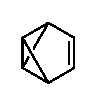
\includegraphics[width=0.1\linewidth]{b.eps} \label{b}}  
\hspace{4ex}
\subfigure[]{
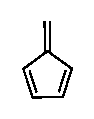
\includegraphics[width=0.1\linewidth]{f.eps} \label{f}}
\hspace{4ex}
\subfigure[]{
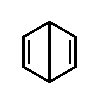
\includegraphics[width=0.1\linewidth]{bD.eps} \label{bD}}  
\caption{\subref{b} бензвален; \subref{f} фульвен; \subref{bD} бензол Дьюара} \label{iso}
\end{figure}

При фотолизе бензола в газовой фазе излучением с длиной волны 193~нм образуются фульвен, {\it цис}- и {\it транс}\nobreakdash-гексадиен\nobreakdash-1,3\nobreakdash-ин\nobreakdash-5, небольшие количества фенильного радикала, однако не 
образуется бензвален и бензол Дьюара \cite{Ward1968a, Kaplan1968a, Tsai2000}. Было сделано предположение, что бензвален и бензол Дьюара формируются из колебательно-возбуждённого основного электронного состояния 
молекулы бензола (так называемого <<горячего бензола>>) \cite{Ward1968a, Nakashima1989, Yatsuhashi2001}. Таким образом, их образование возможно, если электронно-возбуждённая молекула бензола претерпевает безызлучательную конверсию в состояние S$_0$.
Данный процесс эффективно протекает в жидкости из-за межмолекулярных столкновений. В газовой фазе этот процесс неэффективен, потому образуется только термически стабильный фульвен
и продукты фотодиссоциации (таких как, ацетилен, пропилен, гексадиен-1,3-ин-5 и др.) \cite{Bryce-Smith1976}. Известно, что {\it транс}\nobreakdash-гексадиен\nobreakdash-1,3\nobreakdash-ин\nobreakdash-5 под действием излучения с длиной волны 254 нм переходит в {\it цис}-изомер. Гексадиен\nobreakdash-1,3\nobreakdash-ин\nobreakdash-5 затем под действием такого же излучения изомеризуется в бензол и фульвен \cite{Bryce-Smith1976}.


Фотолиз бензола в матрицах изучен мало. Так, в работе \cite{Johnstone1991} описан УФ-фотолиз бензола в матрице твёрдого аргона. При использовании излучения с длиной волны 254~нм 
по данным ИК-спектроскопии первичными продуктами являются фульвен, бензвален и бензол Дьюара (накапливаются линейно с увеличением времени фотолиза). Эксперимент был повторён в матрице ксенона, однако продуктов фотолиза не наблюдалось.
Авторами сделано предположение, что состояние T$_1$ не является предшественником бензола Дьюара, так как в матрице ксенона из-за эффекта тяжёлого
атома выход данного состояния должен быть высоким, однако образования бензола Дьюара не наблюдалось. Для его образования в матрице аргона 
предложен механизм, включающий смешение S$_1$ и S$_2$ состояний, вызванное матрицей. Показано, что при фотолизе бензола в матрице аргона кривая накопления бензвалена со временем выходит на стационарное значение концентрации.
Сделано предположение, что полученный бензвален разлагается при фотолизе с образованием бензола и фульвена. Этот вывод согласуется с ранее полученными данными по фотолизу бензвалена в газовой фазе \cite{Kaplan1968, Harman1981}.  

В работе \cite{Laboy1993} сообщается, что фотолиз осаждённых смесей бензол/аргон и бензол-$d_6$/аргон (в соотношениях от 1:250 до 1:2000) лазером с длиной волны излучения 193~нм не приводит к образованию продуктов по данным ИК-спектроскопии.
Авторы применили фотолиз газовой смеси в процессе осаждения на холодную подложку. При такой постановке эксперимента наблюдались продукты изомеризации и фрагментации бензола.
Показано наличие таких изомеров, как фульвен, бензвален, бензол Дьюара и призман. Среди продуктов фрагментации названы бензин, пропин, 1,3-бутадиин, 
гексатриин, ацетилен и этилен. Кроме того, малоинтенсивная полоса с волновым числом 708~см$^{-1}$ отнесена к фенильному радикалу. Показано, что отношение выходов 
изомеризации и фрагментации бензола зависит от его концентрации в матрице: роль фрагментации значительна при низких концентрациях бензола, изомеризация преобладает в случае больших концентраций.  
Авторы объясняют это различной эффективностью передачи возбуждения в зависимости от концентрации бензола. 
Так, при малой концентрации релаксация неэффективна и быстро протекает
фрагментация, а при большой концентрации эффективность релаксации повышается за счёт столкновений возбуждённых молекул бензола с невозбуждёнными в процессе осаждения. 
Столкновения возбуждённых 
молекул бензола с атомами аргона, конечно, происходят во всех случаях, однако передача энергии не происходит из-за более низкого потенциала 
возбуждения бензола, чем аргона. Кроме того, авторы отмечают отсутствие бензола Дьюара
в экспериментах с низкой концентрацией бензола. Основываясь на этом, они полагают, что в образовании данного продукта принимают участие две молекулы бензола.
Описанная концентрационная зависимость полос была применена авторами к фотолизу дейтеробензола. Полосы продуктов были разделены на две группы, относимые к продуктам изомеризации и фрагментации.
Авторы по имеющимся на тот момент литературным данным относят некоторые серии полос к CD$_3$C$\equiv$CD, DC$\equiv$C--C$\equiv$CD, C$_6$D$_4$ и CD$_2$=CD$_2$. 

В 2015 году опубликована работа \cite{Toh2015}, в которой изучали фотолиз бензола в матрице твёрдого {\it пара}-водорода при помощи ИК-спектроскопии. Использовали излучение с длинами волн 193.0 и 253.7~нм. Основными продуктами фотолиза названы изомеры бензола: 
фульвен, бензол Дьюара и бензвален. Авторы называют первичными продуктами при фотолизе излучением с длиной волны 193.0~нм все три изомера на основании линейных зависимостей их концентраций от времени фотолиза. 
При использовании излучения с длиной волны 253.7~нм фульвен, в отличие от двух других изомеров, не появляется при малых временах фотолиза. Авторы 
делают вывод о том, что фульвен образуется из бензвалена, что согласуется с  более ранними исследованиями, в которых было показано, что фотолиз бензвалена излучением 
с длиной волны 253.7~нм приводит к образованию смеси бензола и фульвена в отношении 3:1 \cite{Kaplan1968, Harman1981}. 
Теоретически предсказана возможность образования и фульвена, и бензвалена из состояния S$_1$ через один и тот же предшественник (<<префульвен>>) \cite{Dreyer1996, Jano1968}, однако эксперименты авторов \cite{Toh2015} её не подтвердили.
Кроме того, в процессе фотолиза бензола в матрице {\it пара}-водорода зафиксирован циклогексадиенильный радикал, который претерпевает раскрытие цикла с образованием гексатриена\nobreakdash-1,3,5. 
Были зафиксированы {\it о}-бензин и гексадиен\nobreakdash-1,3\nobreakdash-ин\nobreakdash-5, образующиеся в малых концентрациях при фотолизе бензола. 
 
 Таким образом, в большом количестве работ по фотолизу бензола в газовой и жидкой фазах установлено образование продуктов фрагментации и изомеризации. Однако фотолизу бензола в условиях матричной изоляции посвящены лишь отдельные работы.
  
\vspace{1cm}
 Проведённый обзор литературы позволяет заключить, что бензол считается радиационно стойким; при этом мнение о его радиационной стойкости
 основано на крайне низких (по сравнению с алифатическими углеводородами) радиационно-химическими выходах газообразных продуктов при радиолизе в конденсированных фазах. Однако вопрос, обусловлена ли радиационная стойкость бензола его <<молекулярными>> свойствами или является следствием взаимодействия их молекул   с окружением, остаётся открытым. Для ответа на этот вопрос могут быть использованы эксперименты с использованием метода матричной изоляции, которая позволяет изучать свойства молекулы в инертном жёстком окружении. Кроме того, при использовании этого метода можно постадийно изучать механизмы радиолиза,
так как в условиях матричной изоляции высокореакционные интермедиаты могут быть стабилизированы и доступны для спектроскопического изучения.
   Однако работы, в которых обсуждалась возможная природа стойкости бензола на молекулярном уровне, единичны. Представления о начальных стадиях радиолиза бензола расплывчаты, данные о механизме радиолиза в бензола в матрицах отрывочны. Известно, что выходы продуктов при радиолизе бензола-$d_6$ ниже, чем при радиолизе недейтерированного аналога, однако влияние  дейтерирования на соотношение основных каналов радиолиза не установлено.
 
 Исходя из вышесказанного, в данной работе были поставлены следующие задачи:
 \begin{itemize}
\item определение состава радикальных и молекулярных продуктов радиолиза бензола в матрицах твёрдых благородных газов;
\item установление основных каналов радиационно-химических превращений молекул бензола в матрицах;
\item выявление влияния характеристик инертной матрицы на эффективность и механизм радиолиза бензола;
\item установление влияния изотопозамещения на основные каналы радиационно-химических превращений бензола в условиях матричной изоляции.
\end{itemize}
 
 }


 
 
 
 
 
 
 
 
 
 
 
 
 

 
 
 
 
 
 
 
 


\newpage
\section{Экспериментальная часть}
Экспериментальная методика, использованная в данной работе, предусматривает несколько основных этапов: 
приготовление газовой смеси необходимой концентрации; получение твёрдого образца путём осаждения газа на холодную подложку криостата; 
облучение рентгеновским излучением; запись ИК-спектров.
\subsection{Используемые вещества}
В качестве матриц применяли благородные газы Ne (99.996\%), Ar (99.998\%), Kr (99.99\%), Xe (99.9996\%) без дополнительной очистки. Бензол (ХЧ, Lachema, Chemapol), бензол-$d_6$ (99.6 атом \% D, Sigma-Aldrich Chemie GmbH) использованы без дополнительной очистки.
\subsection{Приготовление газовых смесей}
Приготовление газовых смесей\footnote{вед. инж. И. В. Тюльпина} осуществляли с помощью установки, 
изображённой на рисунке~\ref{gas}. Мольное соотношение компонентов смеси ($n_1/n_2$) определяли в приближении идеального газа: $n_1/n_2=p_1V_1/p_2V_2$, 
где $V_1$ и $V_2$~--- объёмы, заполняемые газами; $p_1$ и $p_2$~--- давления каждого газа. Установку предварительно вакуумировали до остаточного давления 0.1~Па, 
малую калибровочную ёмкость заполняли исследуемым газом (паром) до необходимого давления и вымораживали в газовую ампулу-приёмник. 
Большую калибровочную ёмкость использовали для отбора матричного газа, который затем также вымораживали в ампулу-приёмник.
\newpage
\begin{figure}[H]
\center{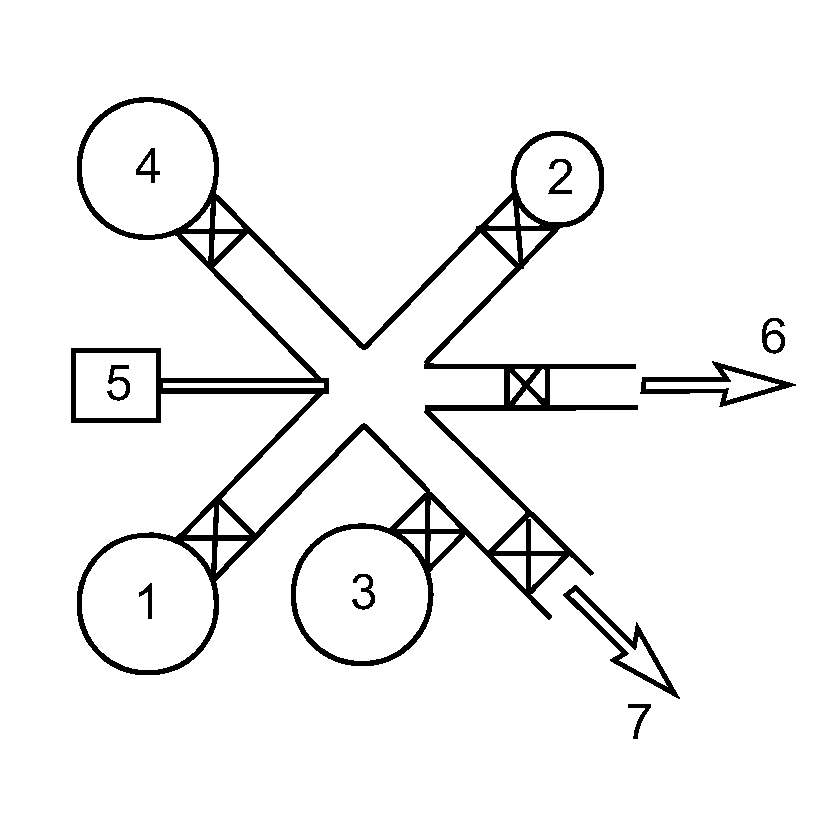
\includegraphics[width=0.5\linewidth]{vu_.pdf}}
\caption{Схема установки для приготовления газовых смесей. 1~--- ампула с исследуемым веществом; 2~--- малая ёмкость с калиброванным объёмом; 3~--- большая ёмкость с калиброванным объёмом; 4~--- ампула для готовой газовой смеси; 5~--- манометр; 6~--- подключение вакуумного поста; 7~--- подключение баллона с матричным газом.}
\label{gas}
\end{figure}
\subsection{Криостат}
В настоящей работе применяли метод ИК-спектроскопии в условиях матричной изоляции. 
Методика экспериментов основана на использовании гелиевого криостата оригинальной конструкции, разработанного в лаборатории химии высоких энергий 
Химического факультета МГУ, на основе серийного криорефрижератора замкнутого цикла Sumimoto Heavy Ind. SRDK-101D-A11C. 
Принципиальная схема криостата изображена на рисунке~\ref{IR}.
Нагнетаемый компрессором гелий расширяется в ступенях рефрижератора, охлаждая криостат. 
Температуру измеряли при помощи термопары медь/медь-железо, обладающей высокой чувствительностью в области гелиевых температур. 
Для регулировки температуры использовали два нагревателя, подключённые к источнику постоянного тока и цифровой контроллер t-Stat. 
Заданная температура поддерживалась с точностью 0.5~К. Измерение температуры осуществляли при помощи контроллеров t-Stat и LakeShore. 
Для измерения давления использовали термопарные лампы ПМТ-2 с вакууметрами Мерадат. Давление внутри криостата не превышало 10$^{-4}$~кПа. 
Криостат для исследований методом ИК-спектроскопии оснащён подложкой для образца, изготовленной из KBr, окошками из КРС для записи ИК-спектров, 
окошком из алюминиевой фольги для облучения рентгеновским излучением, кварцевыми окошками для фотолиза видимым и ближним УФ-излучением.
\begin{figure}[H]
\center{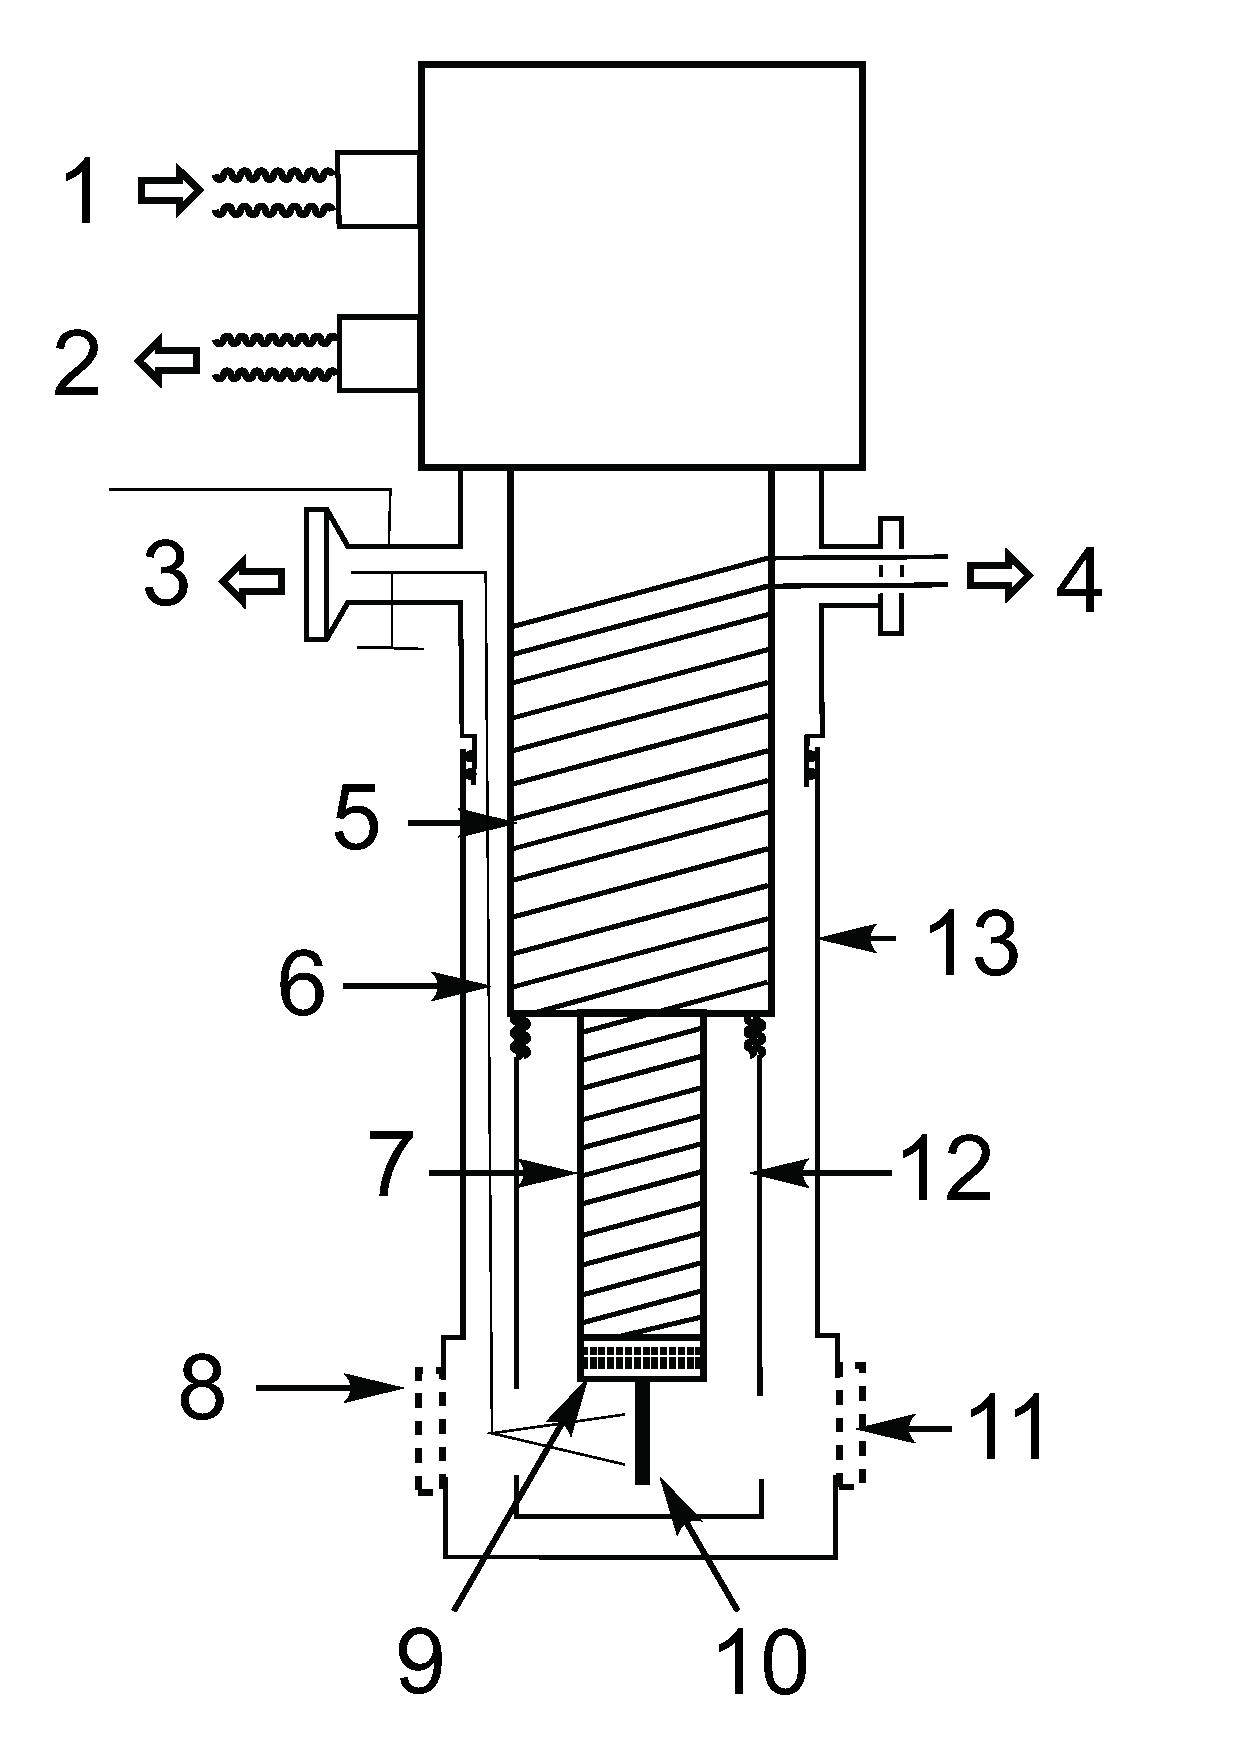
\includegraphics[width=0.6\linewidth]{cryo_numb.pdf}}
\caption{Схема гелиевого криостата замкнутого цикла для проведения исследований. 1 и 2~--- вход и выход компрессора со сжатым гелием; 3~--- подключение вакуумной линии и установки осаждения; 4~--- подключение термоконтроллера; 5~--- первая ступень охлаждения (300--44~K); 6~--- капилляр для осаждения образца; 7~--- вторая ступень охлаждения (44--6~K); 8~--- оптическое окно из КРС-5; 9~--- нагреватель~2; 10~--- подложка из KBr для осаждения образца, держатель, термопара Cu/Fe-Cu, нагреватель~1; 11~--- направление луча ИК-спектрометра; 12~--- защитный экран от теплового излучения; 13~--- вращающийся вакуумный кожух.}
\label{IR}
\end{figure}
\subsection{Осаждение образца и определение толщины слоя}
Для приготовления образца газовую смесь медленно осаждали на охлаждённую подложку криостата, используемая установка изображена на рисунке~\ref{dep}. 
Температуру подложки устанавливали до начала осаждения таким образом, чтобы получить образец с наилучшими оптическими свойствами и близким к равномерному 
распределением исследуемых молекул внутри матрицы. Типичные температуры, использованные для получения матриц в данной работе, составляют 
15--18~K для Ar, 21--25~K для Kr и 25--30~K для Xe. Газовую смесь пропускали через вентиль тонкой регулировки, который позволяет регулировать давление 
внутри коммуникации в процессе осаждения. Типичное время напыления образца составляет 1--1.5~часа.
\begin{figure}[H]
\center{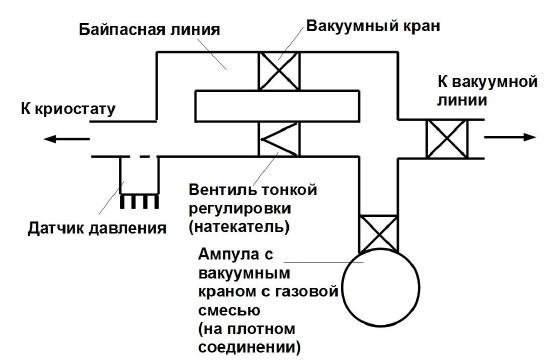
\includegraphics[width=0.6\linewidth]{dep.png}}
\caption{Схема установки подачи газовой смеси в криостат}
\label{dep}
\end{figure}
Толщину образца в ИК-криостате определяли по интерференции, видимой в ИК-спектре (Рисунок~\ref{inter}). 
Интерференция наблюдается при отражении волны от поверхностей раздела фаз: воздух/образец и образец/материал подложки (KBr). 
Отражение происходит при значительном различии коэффициентов преломления двух фаз. Коэффициент преломления воздуха равен 1, 
для  аргона, криптона и ксенона его значения составляют 1.2, 1.3 и 1.4, соответственно~\cite{Sinnock1980}, 
для KBr~--- 1.55. Формула для расчёта толщины слоя: $d = 1/(2n(\nu_1-\nu_2))$, где $d$~--- толщина, $n$~--- коэффициент преломления
матрицы, $(\nu_1-\nu_2)$~--- длина периода интерференции, наблюдаемая в спектре. Толщины образцов в проведённых экспериментах составляют 
120--200~мкм для неоновой матрицы и 70--120~мкм в случае аргона, криптона и ксенона.
\begin{figure}[H]
\center{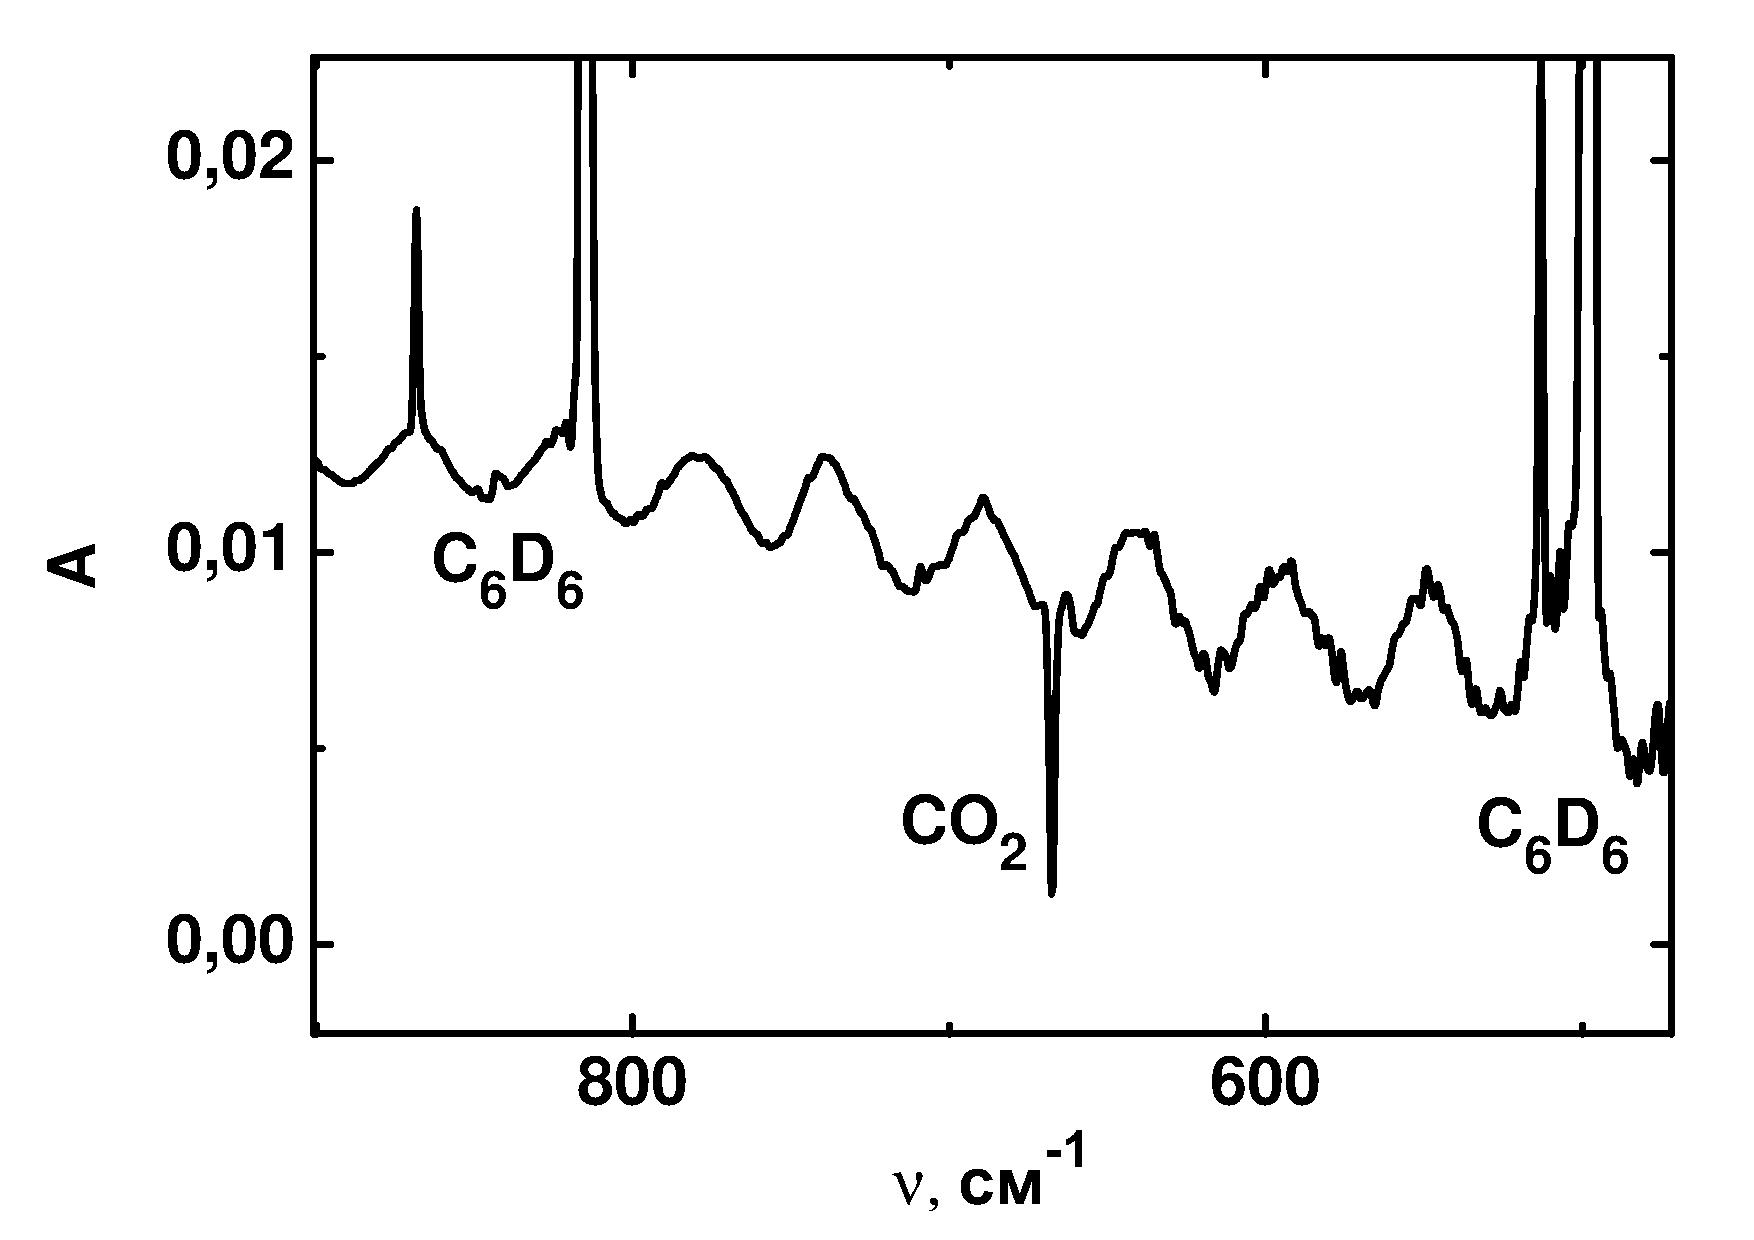
\includegraphics[width=0.8\linewidth]{inter.pdf}}
\caption{Интерференционная картина, наблюдаемая в ИК-спектре осаждённого образца C$_6$D$_6$/Ar}
\label{inter}
\end{figure}
\subsection{Радиолиз и фотолиз}
Осаждённый образец охлаждали до минимальной температуры (5--7~K в зависимости от особенностей сборки криостата) 
и подвергали действию излучения рентгеновской трубки 5-БХВ6-W с вольфрамовым анодом с максимальной энергией кванта около 32~кэВ 
(эффективная энергия составляет примерно 20~кэВ).
Для оценки мощности дозы использовался ферросульфатный дозиметр (дозиметр Фрикке), радиационно-химический выход ионов Fe$^{3+}$
 в котором равен 14.4~иона/100~эВ при эффективной энергии рентгеновского излучения 20~кэВ \cite{Pikaev}. 
 В геометрии облучения образца в ИК-криостате мощность дозы для дозиметрического раствора составила 0.72 Гр/с.
 Полученную величину мощности дозы пересчитывали с учётом массовых коэффициентов поглощения среды для осаждённых плёнок инертных газов 
 по формуле:
$I(\mathrm{Ng}) = \frac{\mu(\mathrm{Ng})\cdot I(\mathrm{H_2O})}{\mu(\mathrm{H_2O})}$, где $I(\mathrm{Ng})$ и $I(\mathrm{H_2O})$~--- мощности дозы для благородного газа и дозиметрического раствора, соответственно, $\mu(\mathrm{Ng})$ и $\mu(\mathrm{H_2O})$~--- массовые коэффициенты поглощения для благородного газа и дозиметрического раствора (последний считается равным коэффициенту для воды). Массовые коэффициенты поглощения и полученные значения мощности дозы представлены в таблице \ref{dose}.
\begin{table}[H]
\caption{Массовые коэффициенты поглощения \cite{xray} и мощности поглощённой дозы в матрицах инертных газов}
\label{dose}
\begin{center}
\begin{tabular}{c|cccc}
 & H$_2$O & Ar & Kr & Xe \\
 \hline
$\mu$, см$^2$/г & 0.55 & 8.1 & 35 & 25 \\
$I$, Гр/с & 0.72 & 11 & 47 & 33 \\
\end{tabular}
\end{center}
\end{table}

Следует, однако, отметить, что приведённые дозиметрические данные (как и рассчитанные на их основе величины радиационно-химических выходов) 
носят оценочный характер, поскольку спектр излучения имеет непрерывный характер, а массовые коэффициенты поглощения очень сильно (и притом немонотонно)
 зависят от энергии фотона в этой области. Кроме того, даже при толщинах осаждённого слоя до 100~мкм в криптоне и ксеноне возникает заметная 
 неоднородность распределения дозы по толщине образца (по этой причине использование более толстых слоёв нецелесообразно).

Фотолиз в видимой и ближней УФ областях проводили при помощи узкополосных диодных источников через кварцевые окошки криостата. 
Длины волн максимумов испускания использованных диодов приведены в таблице \ref{diod}.

Фотолиз в УФ области проводили при помощи ртутных газоразрядных ламп низкого и среднего давлений
ОУФ-6  и ОУФв\nobreakdash-02 <<Солнышко>>.

\begin{table}[H]
\caption{Длины волн максимумов испускания использованных диодов}
\label{diod}
\begin{center}
\begin{tabular}{lc}
Диод & Длина волны, нм \\
\hline
Красный & 625 \\
Оранжевый & 605 \\
Жёлтый & 590 \\
Зелёный & 525 \\
Синий & 460 \\
УФ & 400 \\
\end{tabular}
\end{center}
\end{table}

\subsection{Регистрация ИК-спектров}
ИК-спектры регистрировали с помощью Фурье-ИК спектрометра Bruker Tenzor II, снабжённого охлаждаемым жидким азотом полупроводниковым детектором MCT.
Спектры регистрировали в диапазоне волновых чисел 7500--400~см$^{-1}$ с разрешением  
1~см$^{-1}$, что было достаточно для целей эксперимента, и проводили усреднение по 144~сканированиям. 
Управление спектрометром осуществляли при помощи персонального компьютера с использованием программного обеспечения OPUS. 
Все спектры регистрировали при минимальной температуре.
\subsection{Квантово-химические расчёты}
Квантово-химические расчёты выполнены Сосулиным И.С. с использованием метода DFT(PBE). Данный функционал обеспечивает удовлетворительное описание энергетических и геометрических свойств для довольно обширного круга соединений при небольшой вычислительной стоимости \cite{Ernzerhof1999}. Кроме того, показано \cite{Furera2006, POPOV}, что расчёты на уровне PBE/TZ2P с хорошей точностью воспроизводят ИК спектры ароматических и полиароматических соединений. Для проведения расчетов применялся валентный корреляционно-согласованный базисный набор, L2\_3 
\cite{Laikov2005}. 
Базис L2\_3 является аналогом широко известного набора cc-pVTZ 
\cite{Kendall1992}, но отличаются от них большим числом элементарных гауссовых функций. Схема сжатия базисных наборов L2\_3, cc-pVTZ представлена в Приложении А. Данный базисный набор обеспечивает лучшее описание совокупности свойств молекулярных систем, чем аналогичный базис Даннинга. В то же время показано, что при больших n результаты расчётов в базисах Ln\_3 и соответствующих cc-pVXZ базисах сходятся друг к другу \cite{Laikov2005}. Точность самосогласования электронной задачи составляла 10$^{-10}$ а.е., геометрии оптимизировались до нормы градиента 10$^{-6}$ а.е. На оптимизированных геометриях решалась колебательная задача в гармоническом приближении с определением частот колебаний, ИК-интенсивностей и энергии нулевого колебательного уровня. Существование минимума на поверхности потенциальной энергии подтверждалось отсутствием мнимых частот колебаний у данной структуры. Для проведения расчётов использовался пакет программ PRIRODA, любезно предоставленный Д. Н. Лайковым \cite{Laikov}. Проведённые нами неэмпирические расчёты не учитывают влияния среды, то есть формально относятся к молекулам в вакууме (или газовой фазе), что может приводить к некоторому  расхождению экспериментальных и расчётных частот.












\newpage
\section{Результаты и их обсуждение}
\sloppy{
\subsection{Радиолиз бензола}
В ИК-спектрах осаждённых образцов бензола в матрицах аргона, криптона и ксенона присутствуют узкие полосы поглощения,
соответствующие бензолу, их частоты согласуются с литературными данными \cite{Kim1996}. Кроме того, в спектрах осаждённых образцов присутствуют полосы, соответствующие незначительным количествам воды и углекислого газа.
Типичный вид спектра осаждённого образца C$_6$H$_6$/Ng представлен на рисунке~\ref{depAr}.
\begin{figure}[H]
\center{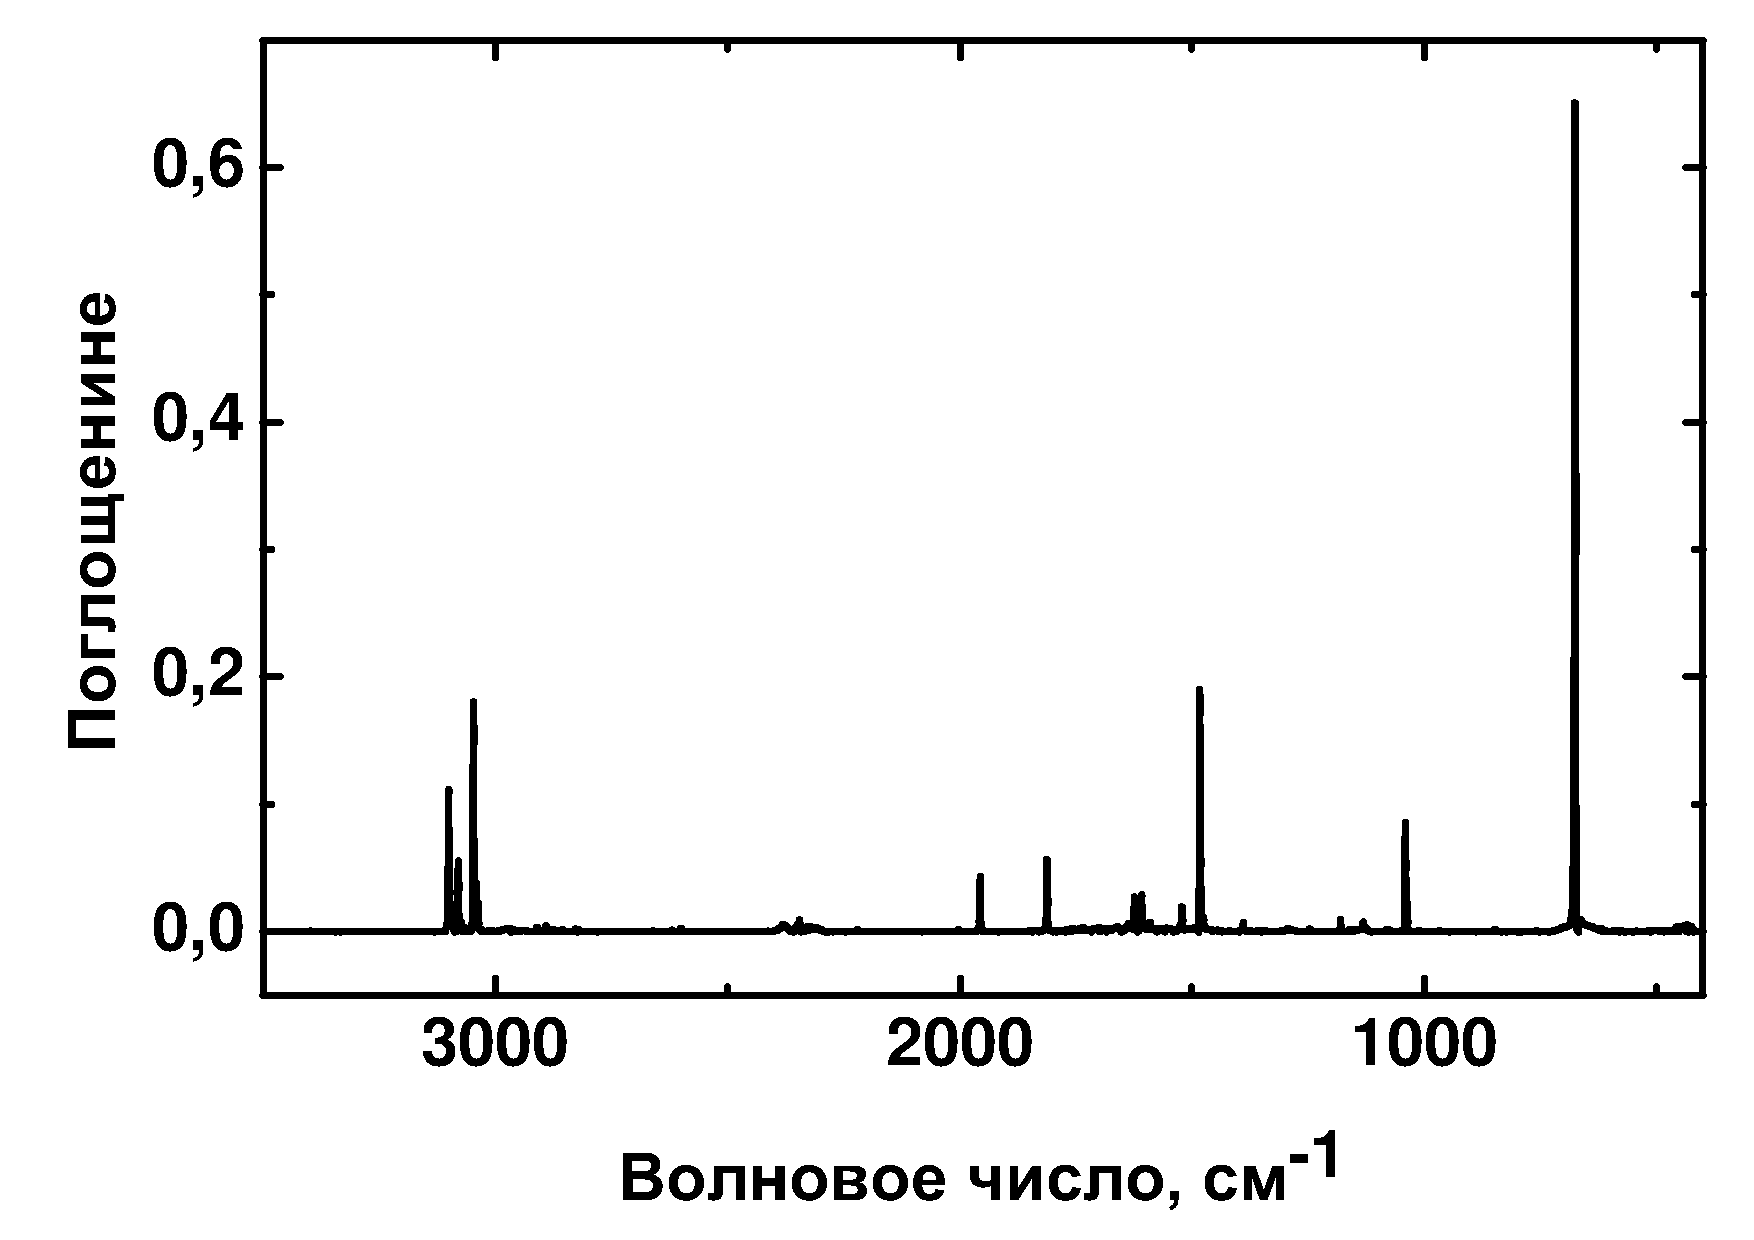
\includegraphics[width=0.9\linewidth]{is.pdf}}
\caption{ИК-спектр осаждённой смеси C$_6$H$_6$/Ar 1:1000}
\label{depAr}
\end{figure}

В результате облучения бензол расходуется во всех матрицах довольно эффективно. Зависимости относительной концентрации бензола (отношение интегральных интенсивностей сигналов
 в облучённом и не облучённом образцах)
  от поглощённой дозы в различных матрицах представлены на рисунке~\ref{conv}.
Использование относительной концентрации бензола в качестве одной из координат позволяет сравнивать результаты, полученные в различных матрицах, без использования коэффициентов 
молярного поглощения, не вносить поправку на различную толщину осаждённого слоя в экспериментах.

\begin{figure}[H]
\center{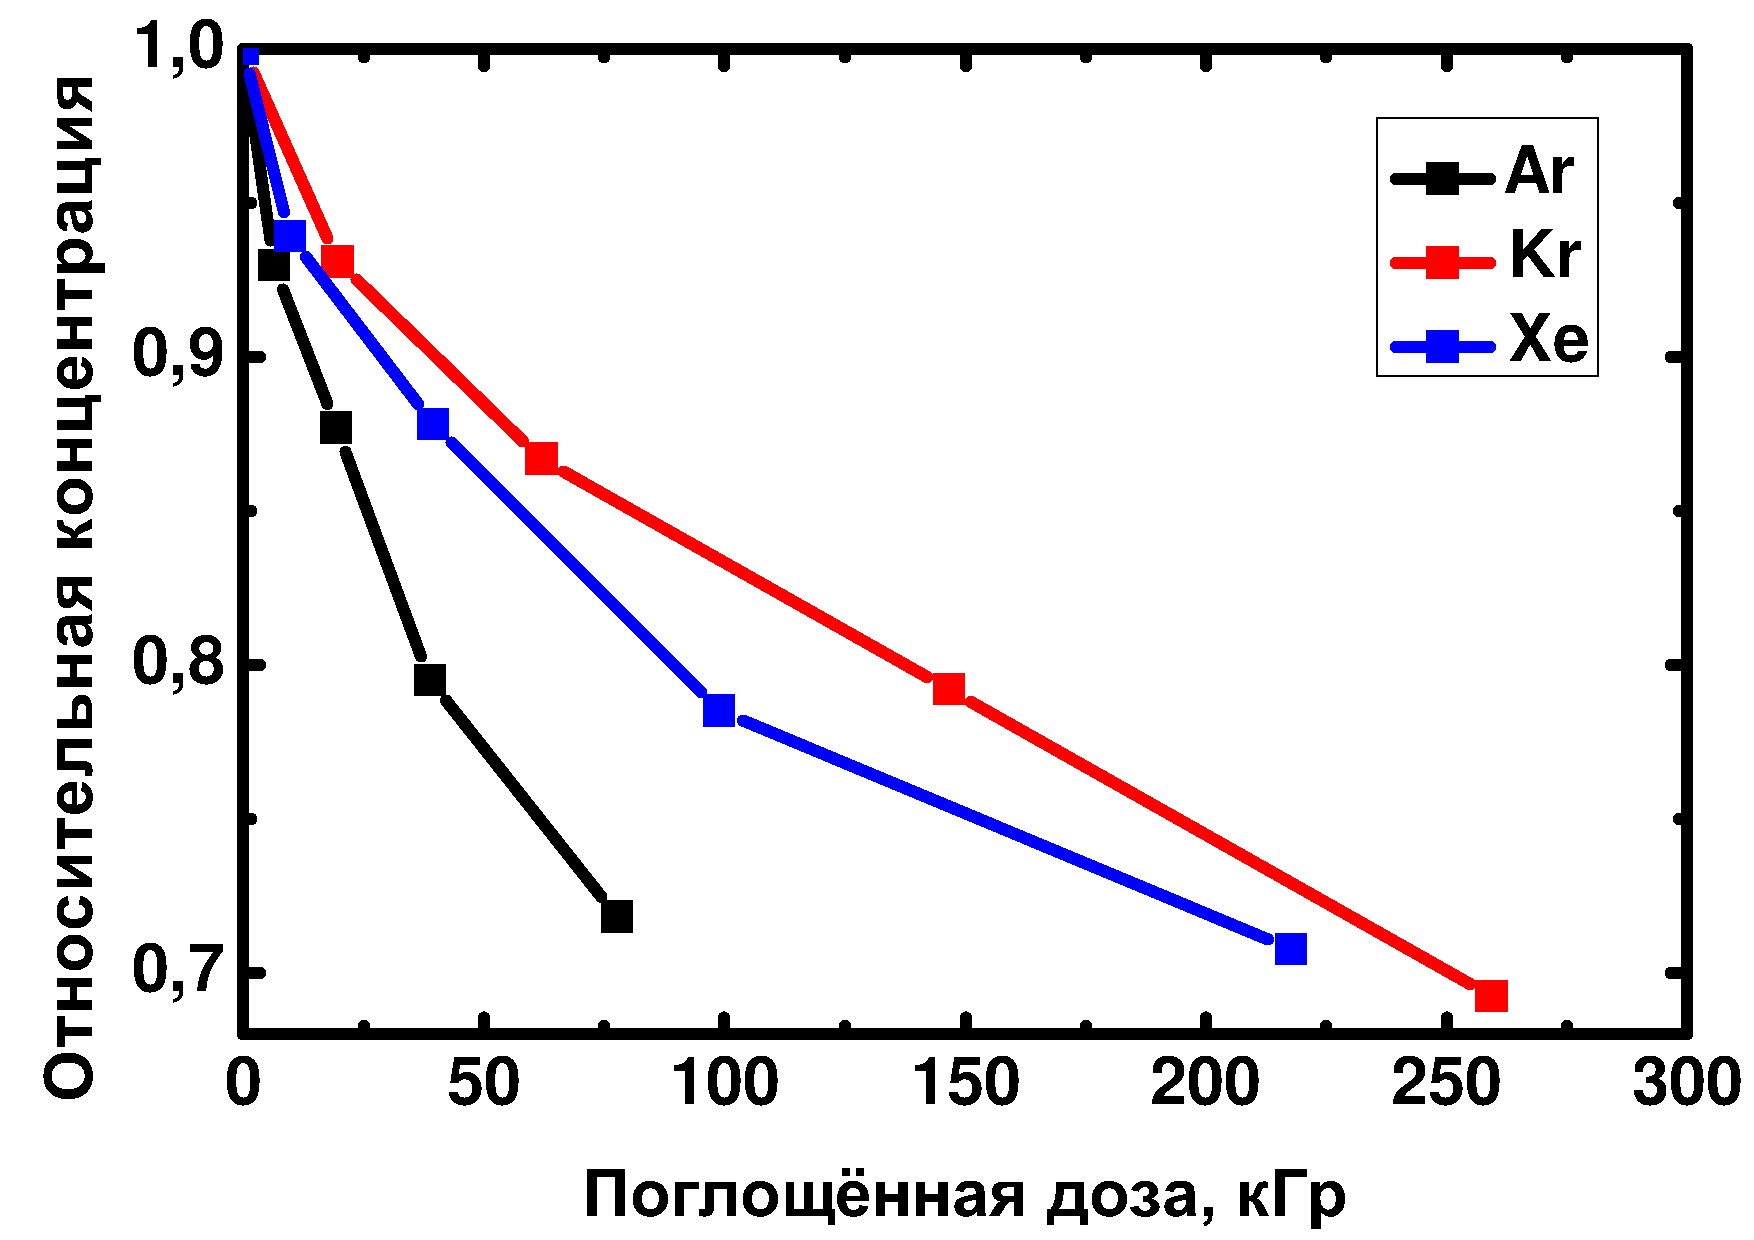
\includegraphics[width=0.8\linewidth]{dose_1.pdf}}
\caption{Кривые расходования бензола в различных матрицах}
\label{conv}
\end{figure}

Разложение бензола в матрице аргона протекает эффективнее, чем в более тяжёлых матрицах (Kr, Xe). Начальные участки всех кривых линейны, при больших дозах (более 100~кГр) в криптоне и ксеноне наблюдается так называемое <<дозовое насыщение>>~---
уменьшение эффективности разложения с увеличением поглощённой дозы. Такой вид зависимости  является типичным для радиолиза большинства веществ, в связи с накоплением продуктов радиолиза и уменьшением концентрации бензола, что снижает эффективность передачи энергии на оставшиеся молекулы бензола. По наклону линейных начальных участков кривых, представленных на рисунке~\ref{conv}, определены радиационно-химические выходы разложения
бензола по формуле:
\begin{equation} \label{yee}
G = \frac{\Delta c}{1000MtI}, 
\end{equation}
где $\Delta c$~--- изменение относительной концентрации бензола, 1000~--- мольное отношение матрицы и бензола, $M$~--- молярная масса матрицы, $t$~--- время облучения, $I$~--- мощность дозы.

Значения выходов составили
2.6~молек./100~эВ в матрице аргона и  0.4~молек./100~эВ в матрицах криптона и ксенона. Радиационно-химический выход разложения бензола сопоставим с 
выходами разложения других молекул в условиях матричной изоляции (см.~раздел~\ref{isolation}), что ставит под вопрос радиационную стойкость бензола, обусловленную его молекулярными свойствами.
 Следует отметить, что радиационно-химический выход разложения бензола в матрицах инертных газов ниже, чем выход разложения бензола при радиолизе в газовой фазе (см.~раздел~\ref{products}), это является типичной ситуацией из-за более лёгкой диссипации энергии в твёрдой фазе по сравнению с газовой.
Понижение выхода разложения бензола при переходе от аргоновой к криптоновой и ксеноновой матрицам, по-видимому, можно объяснить действием двух факторов. 
Во-первых, в тяжёлых матрицах эффективно происходит интеркомбинационная конверсия, из-за чего вклад каналов, 
протекающих через синглетные состояния, значительно уменьшается. Во-вторых, матрицы криптона и ксенона обладают большей поляризуемостью, чем матрица аргона, что приводит
к эффективной релаксации возбуждённых состояний к основному электронному состоянию.


После облучения бензола во всех матрицах в ИК-спектрах появляются новые полосы поглощения (см. рисунок \ref{spectra}).
В таблицах~\ref{tabl:phenyl}, \ref{fulvene} представлены частоты колебаний фенильного радикала и фульвена, соответственно, 
которые появляются после облучения во всех матрицах. Отнесение проведено на основании литературных данных (см. раздел~\ref{rad}) с учётом разумных матричных сдвигов (см. раздел~\ref{isolation}). Кроме того, в ИК-спектрах облучённых образцов присутствует крайне малоинтенсивная радиационно-индуцированная полоса поглощения при 741.1~см$^{-1}$ в матрице аргона и 738.5~см$^{-1}$ в матрице криптона, наличие которой может свидетельствовать об образовании следовых количеств бензвалена. Указанная полоса является наиболее интенсивной для бензвалена, согласно экспериментальным и теоретическим исследованиям. Интенсивность остальных полос поглощения как минимум в три раза ниже~\cite{Toh2015}, а значит они  слишком малы для регистрации и отнесения в условиях нашего эксперимента. Отнесение по одной полосе ненадёжно, поэтому вывод из полученных данных о наличии бензвалена может быть только предварительным. В матрице ксенона полоса поглощения бензвалена может быть слишком мала для регистрации в наших условиях. Из литературы известно, что при фотолизе бензола в аргоне кроме описанных изомеров (фульвена и бензвалена), образуется бензол Дьюара, однако полос, которые можно было бы отнести к нему, ни в одной матрице не наблюдается. Кроме того, во всех матрицах образуется сольватированный протон Ng$_2$H$^+$ 
(Ar$_2$H$^+$: 903.3 и 1139.6~см$^{-1}$; Kr$_2$H$^+$: 852.5, 1007.7 и 1160.4~см$^{-1}$; Xe$_2$H$^+$: 730.6, 842.7 и 953.4~см$^{-1}$; см. раздел~\ref{isolation}). 

\begin{figure}[H]  
\centering 
\hspace{-6ex}
\subfigure[]{
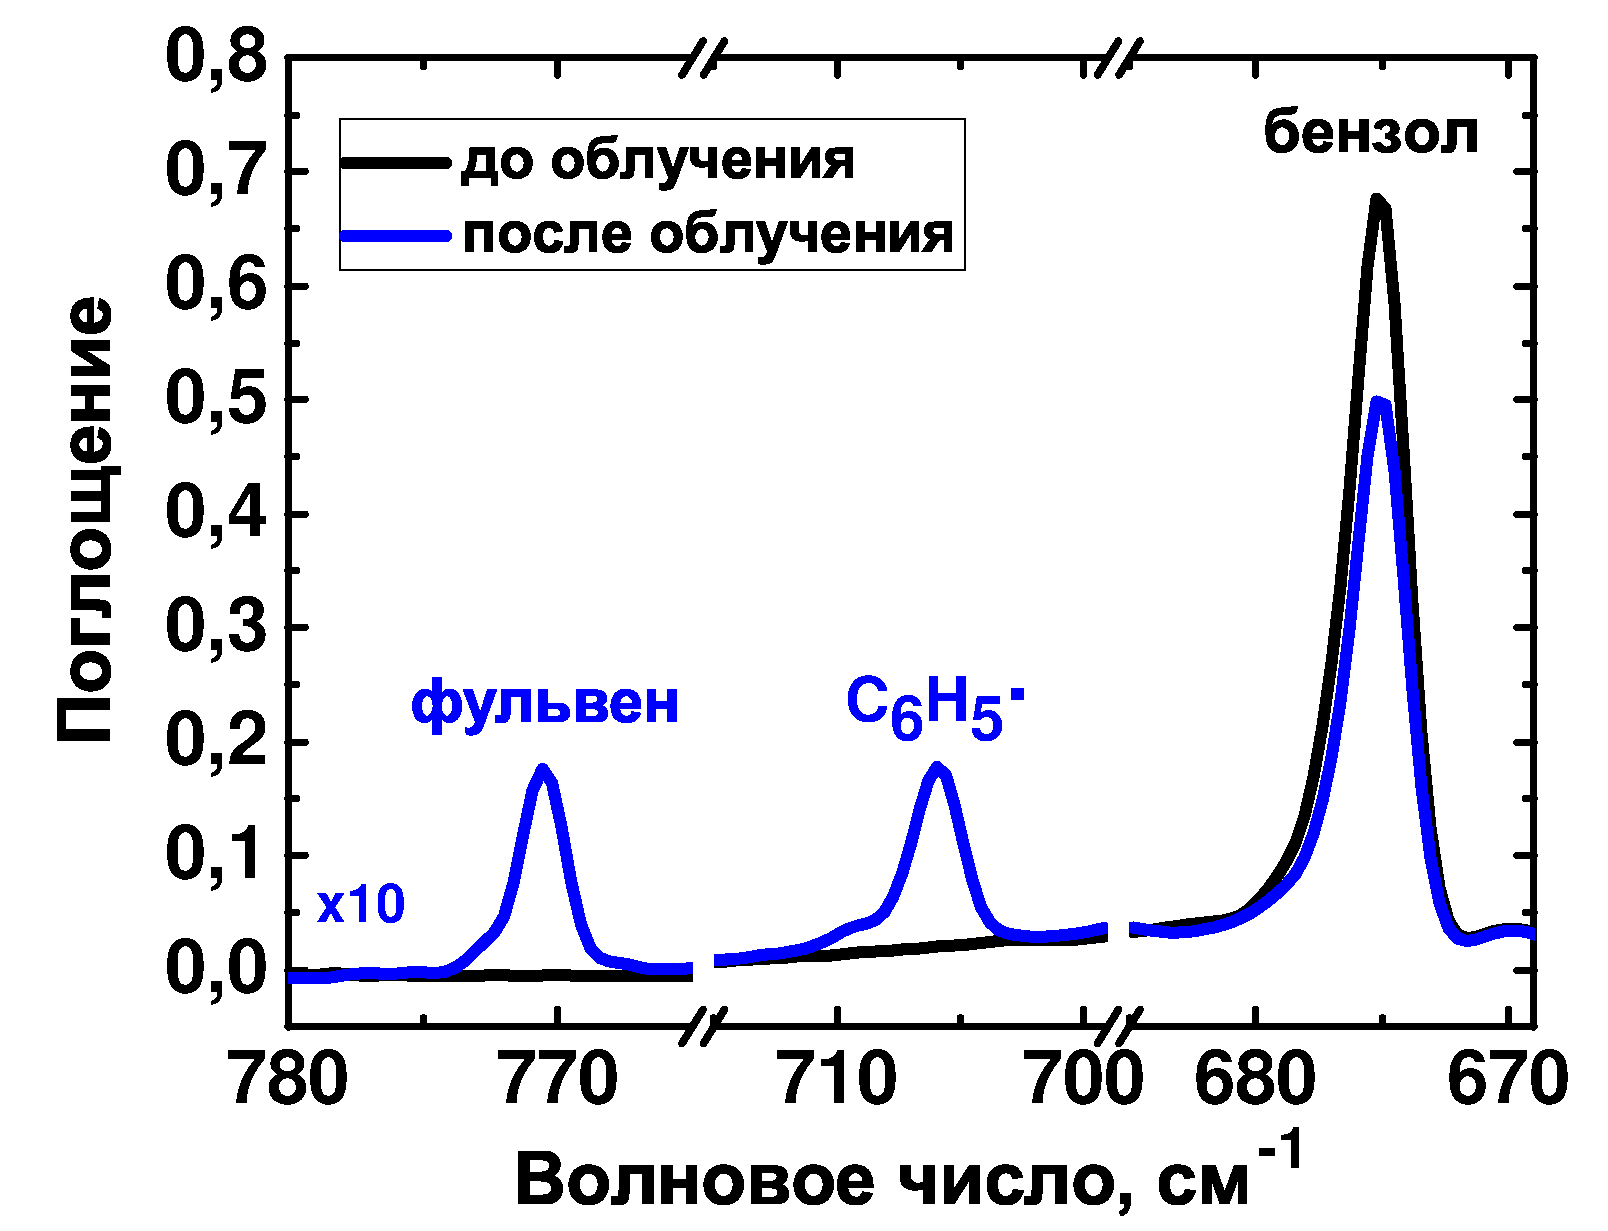
\includegraphics[width=0.5\linewidth]{Ar_sp_irr.pdf} \label{Ar_sp}}  
\subfigure[]{
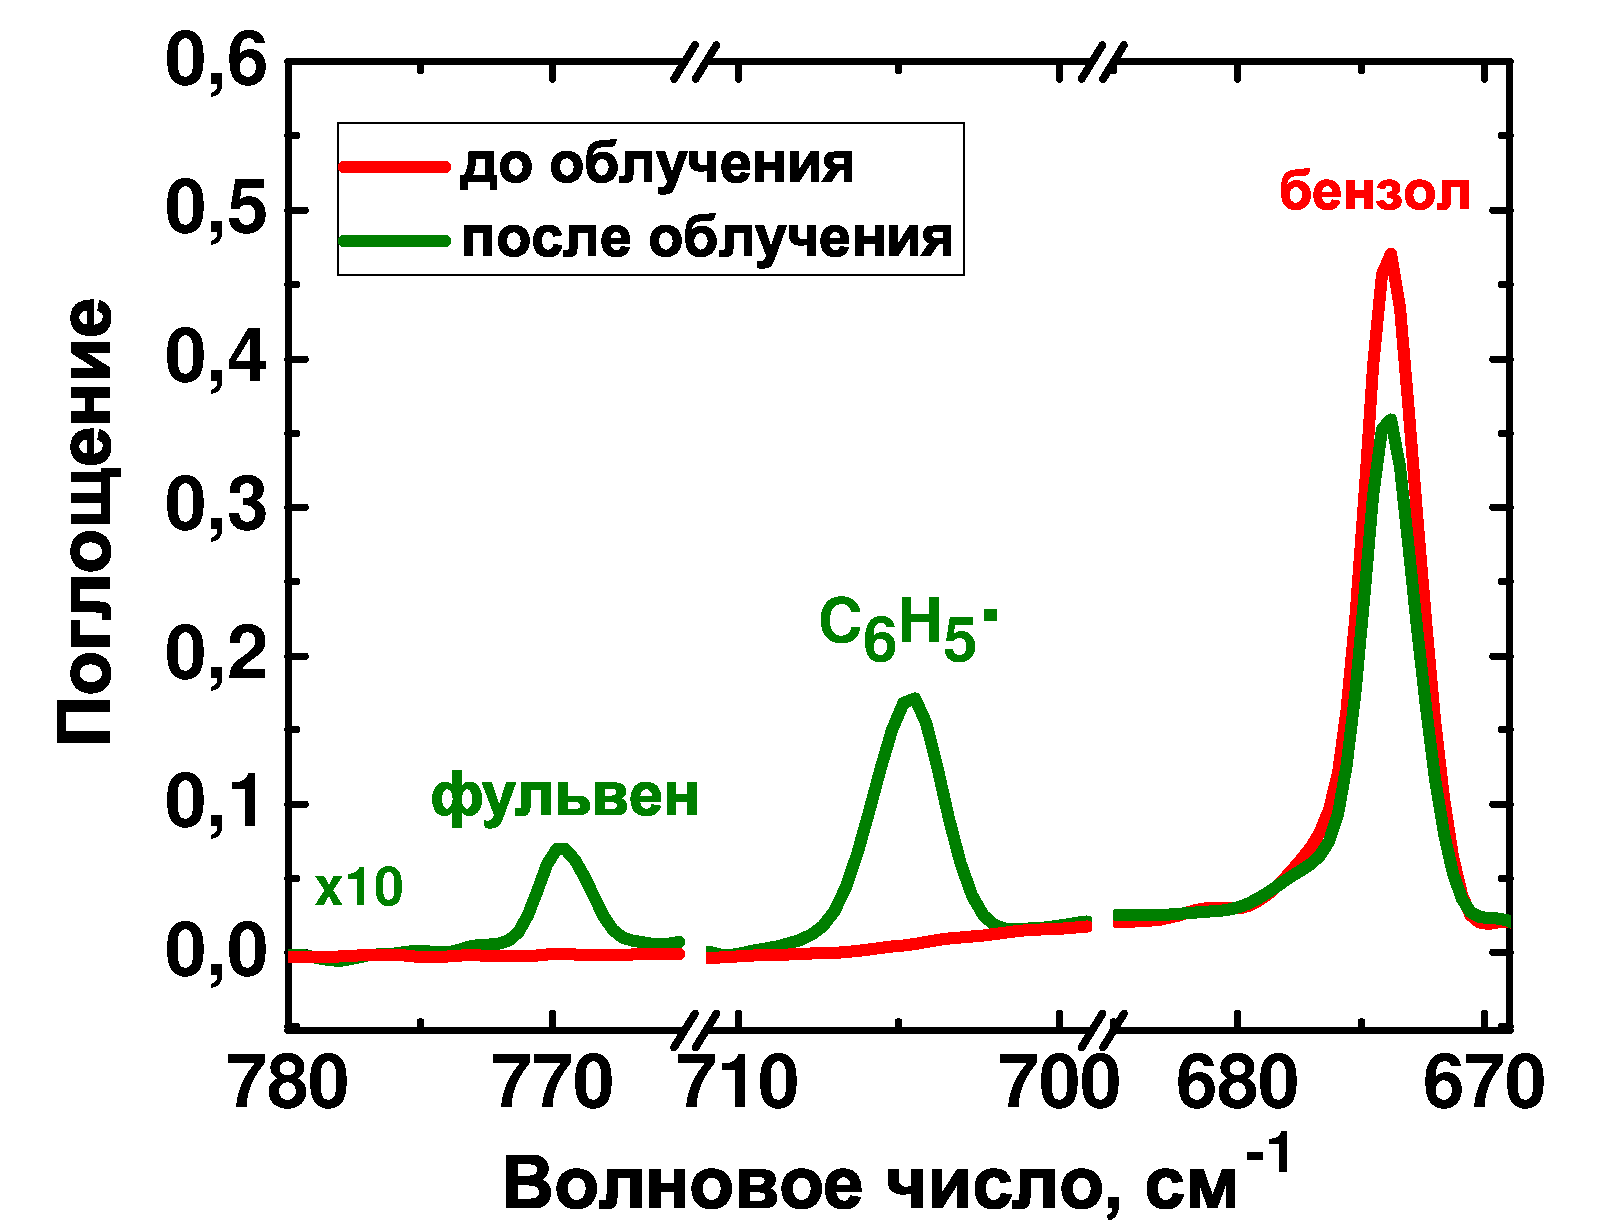
\includegraphics[width=0.5\linewidth]{Kr_sp_irr.pdf} \label{Kr_sp}}
\caption{Фрагменты ИК-спектров бензола в матрицах \subref{Ar_sp}~аргона; \subref{Kr_sp}~криптона до и после облучения} 
\label{spectra}
\end{figure}

\begin{table}[H]
\caption{Волновые числа колебаний фенильного радикала~(см$^{-1}$) в~различных матрицах}
\label{tabl:phenyl}
\begin{center}
\begin{tabular}{ccc}
Ar & Kr & Xe \\
\hline
604.7 & 603.0 & 601.2 \\
657.5 & 656.0 & 654.9 \\
706.0 & 704.8 & 703.9 \\
1026.5 & 1024.8 & 1022.5 \\
1432.2 & 1430.3 & 1429.1 \\
1441.2 & 1439.7 & 1437.9 \\
3087.0 & 3063.8 & 3055.7 \\
\end{tabular}
\end{center}
\end{table}

\begin{table}[H]
\caption{Волновые числа колебаний фульвена~(см$^{-1}$) в~различных матрицах}
\label{fulvene}
\begin{center}
\begin{tabular}{ccc}
Ar & Kr & Xe \\
\hline
616.1 & 615.4 & 614.8 \\
770.6 & 769.7 & 768.6 \\
894.4 & 893.3 & - \\
926.3 & 925.2 & 924.5 \\
1080.9 & - & - \\
1343.0 & 1341.0 & 1339.3 \\
1489.1 & - & - \\
\end{tabular}
\end{center}
\end{table}

Кривые накопления фульвена и фенильного радикала в различных матрицах представлены на рисунке~\ref{tio}. Использовали координаты относительная концентрация продукта -- конверсия бензола (доля разложившегося бензола).
Для получения относительных концентраций каждую интегральную интенсивность сигнала
нормировали на соответствующий молярный коэффициент поглощения, считая, что коэффициент не зависит от матрицы (56~км/моль для внеплоскостных C--H  колебаний фенильного радикала 
(706.0~см$^{-1}$ в~аргоне) по данным эксперимента~\cite{Friderichsen2001}, 50~км/моль  для внеплоскостных C--H колебаний фульвена (770.6~см$^{-1}$ в~аргоне) по данным квантово-химического расчёта без учёта окружения~\cite{Toh2015}). Полученные значения нормировали на максимальную концентрацию фенильного радикала, что необходимо для сравнения данных, которые получены в различных экспериментах в различных матрицах.

Из рисунка~\ref{tio} видно, что в матрицах аргона и криптона оба рассматриваемых продукта появляются сразу после облучения и при малых конверсиях бензола (до 0.1--0.15) накапливаются линейно, а значит они являются первичными.
В матрице ксенона распад бензола на фенильный радикал и атом водорода является доминирующим каналом радиолиза, 
что согласуется с литературными данными (см. раздел~\ref{rad}).
\\
\begin{figure}[H]  
\vspace{-4ex} \centering \subfigure[]{
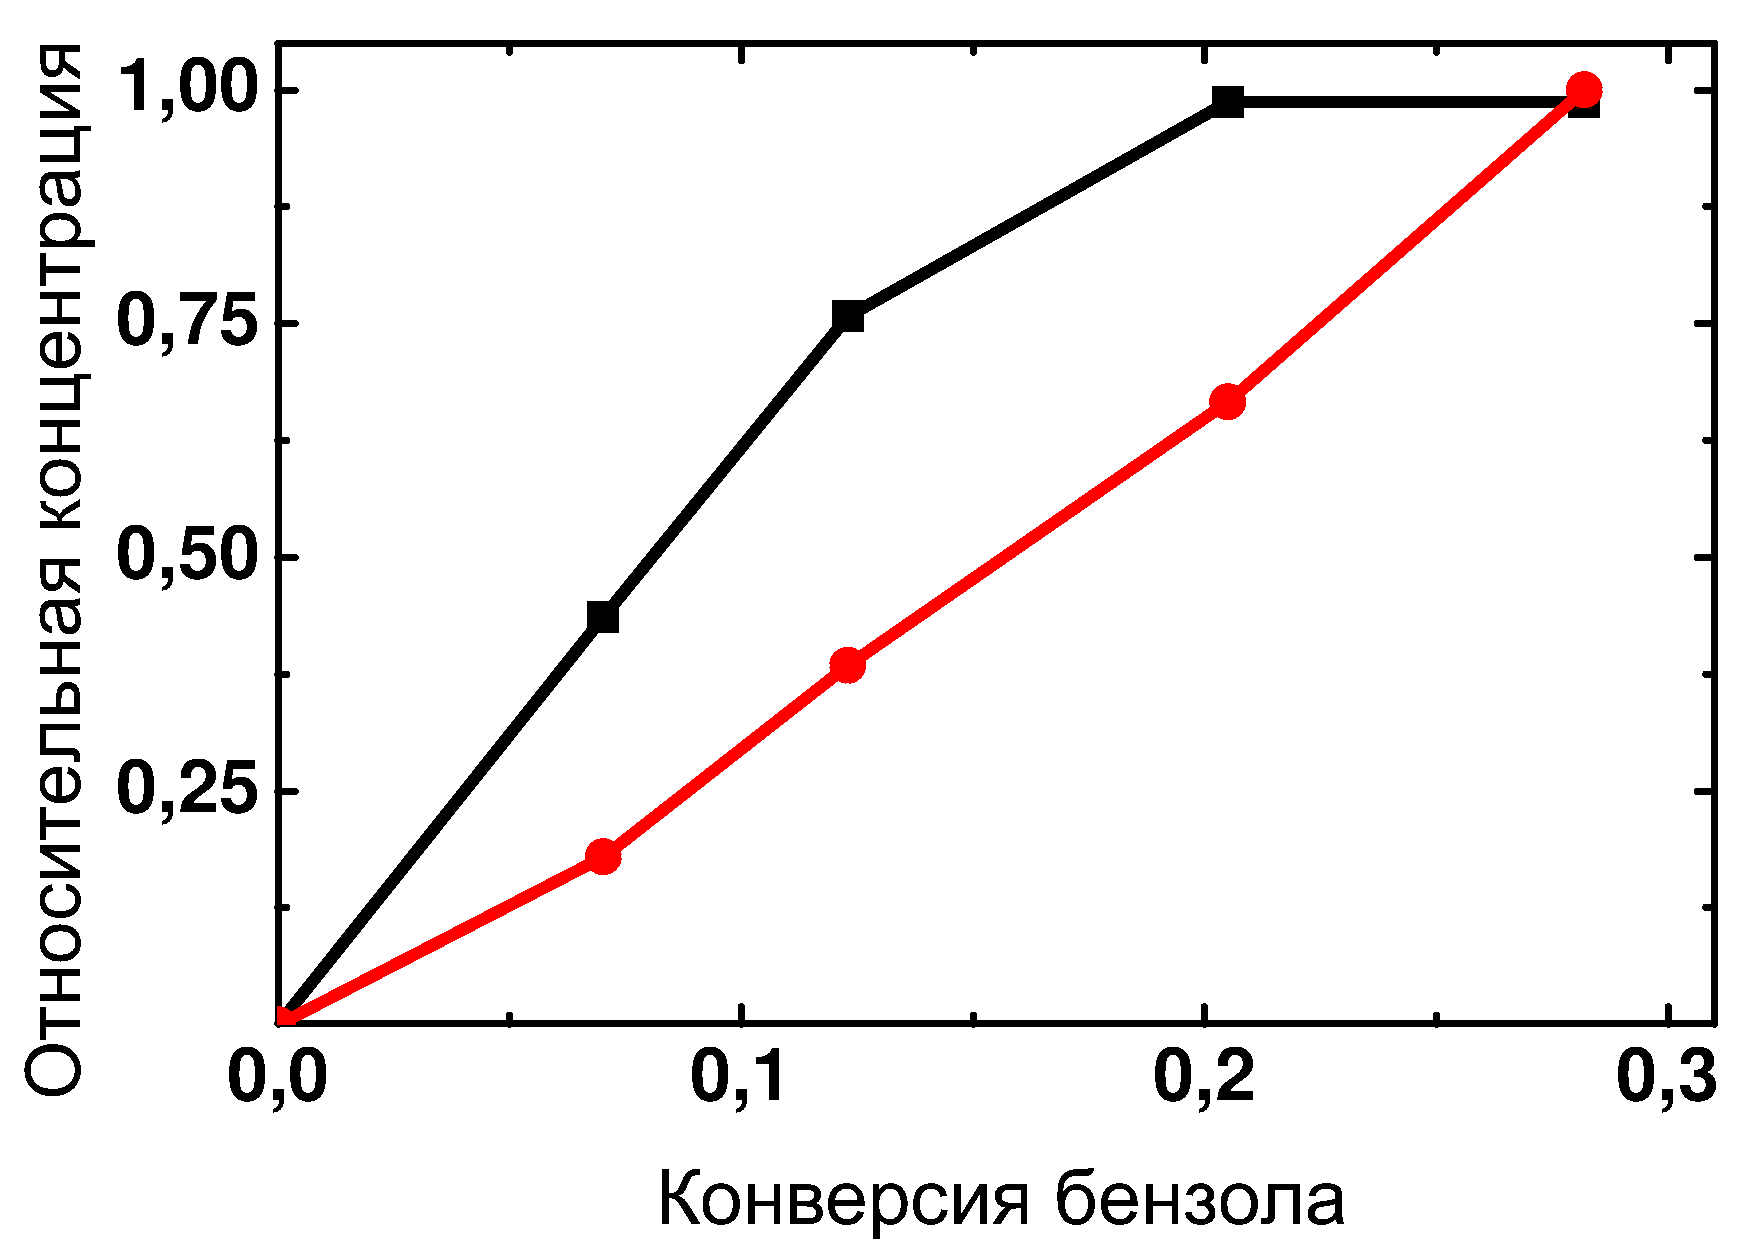
\includegraphics[width=0.6\linewidth]{prodAr+.pdf} \label{prodAr}}  
\hspace{4ex}
\subfigure[]{
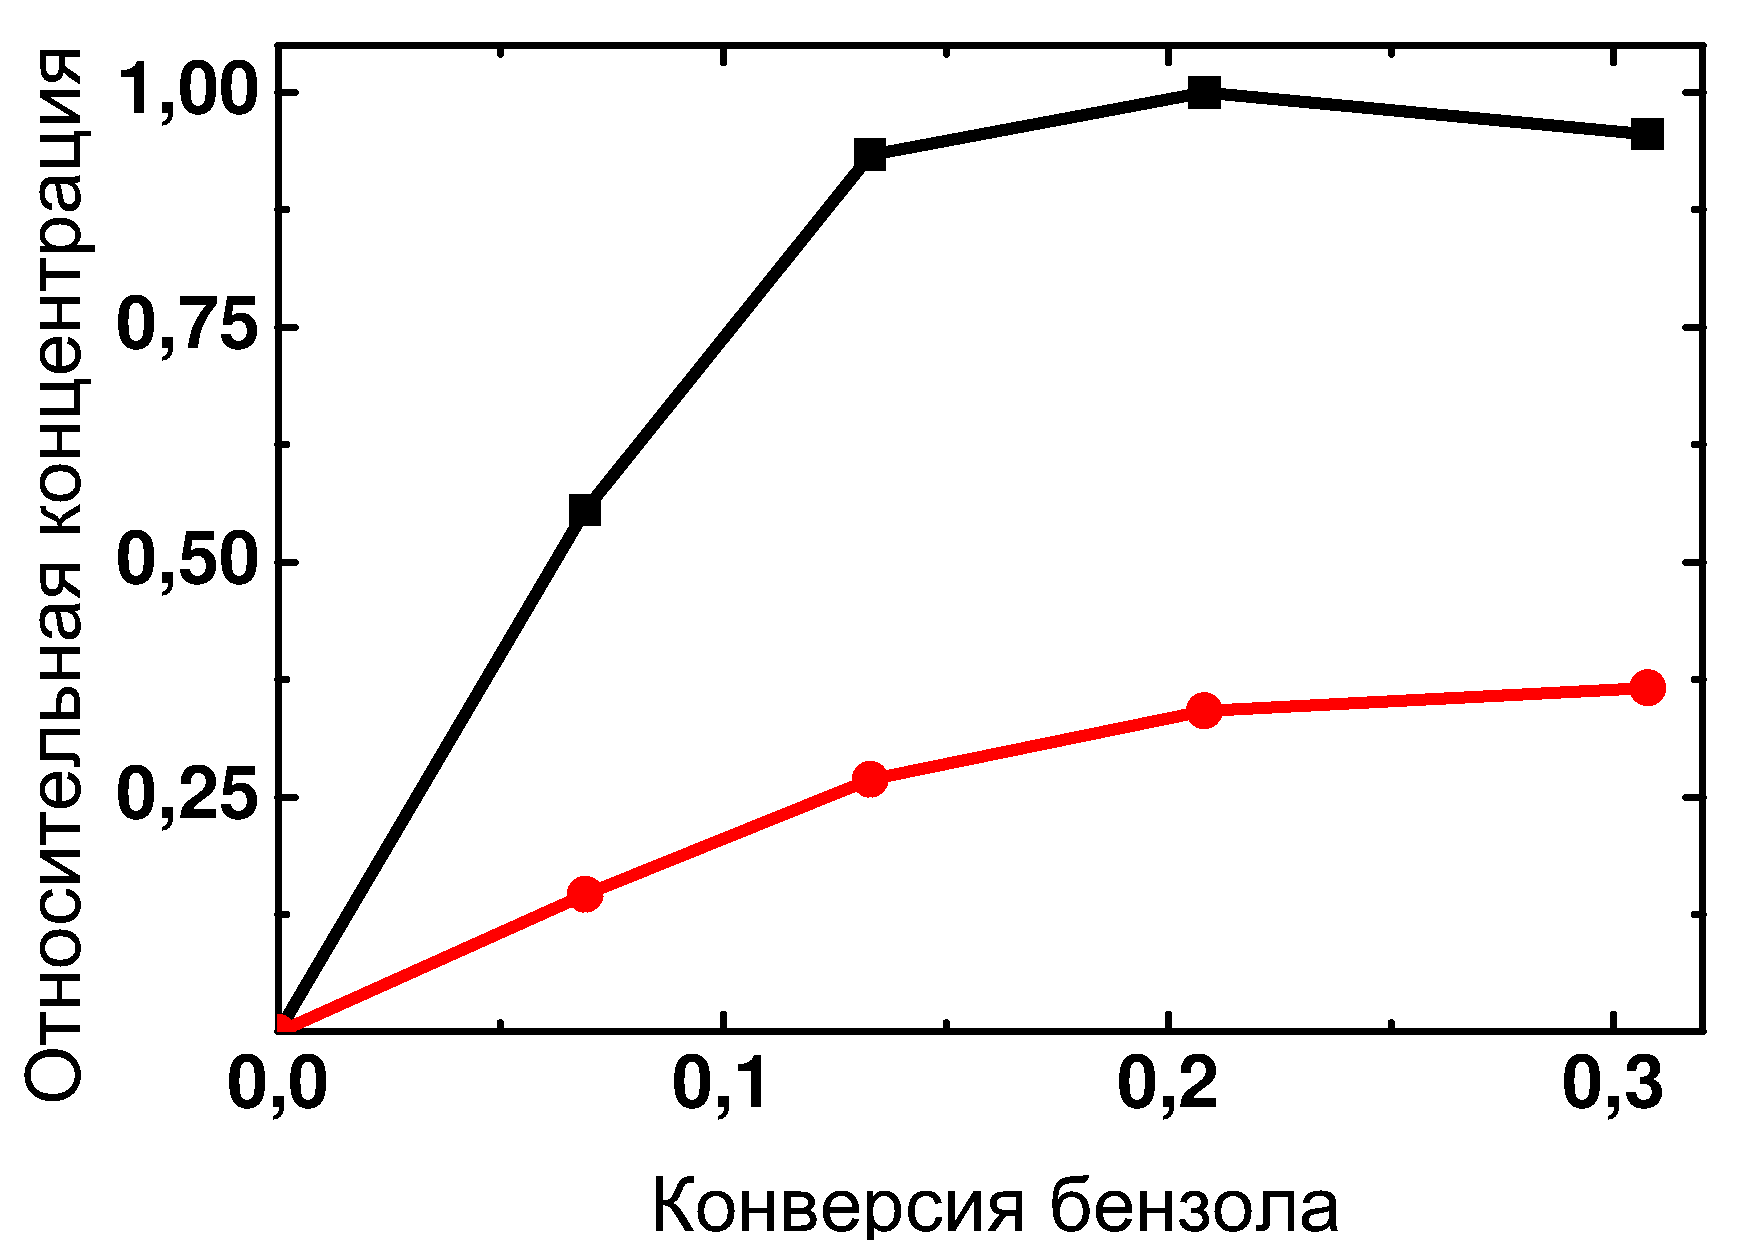
\includegraphics[width=0.6\linewidth]{prodKr+.pdf} \label{prodKr}}
\hspace{4ex}
\subfigure[]{
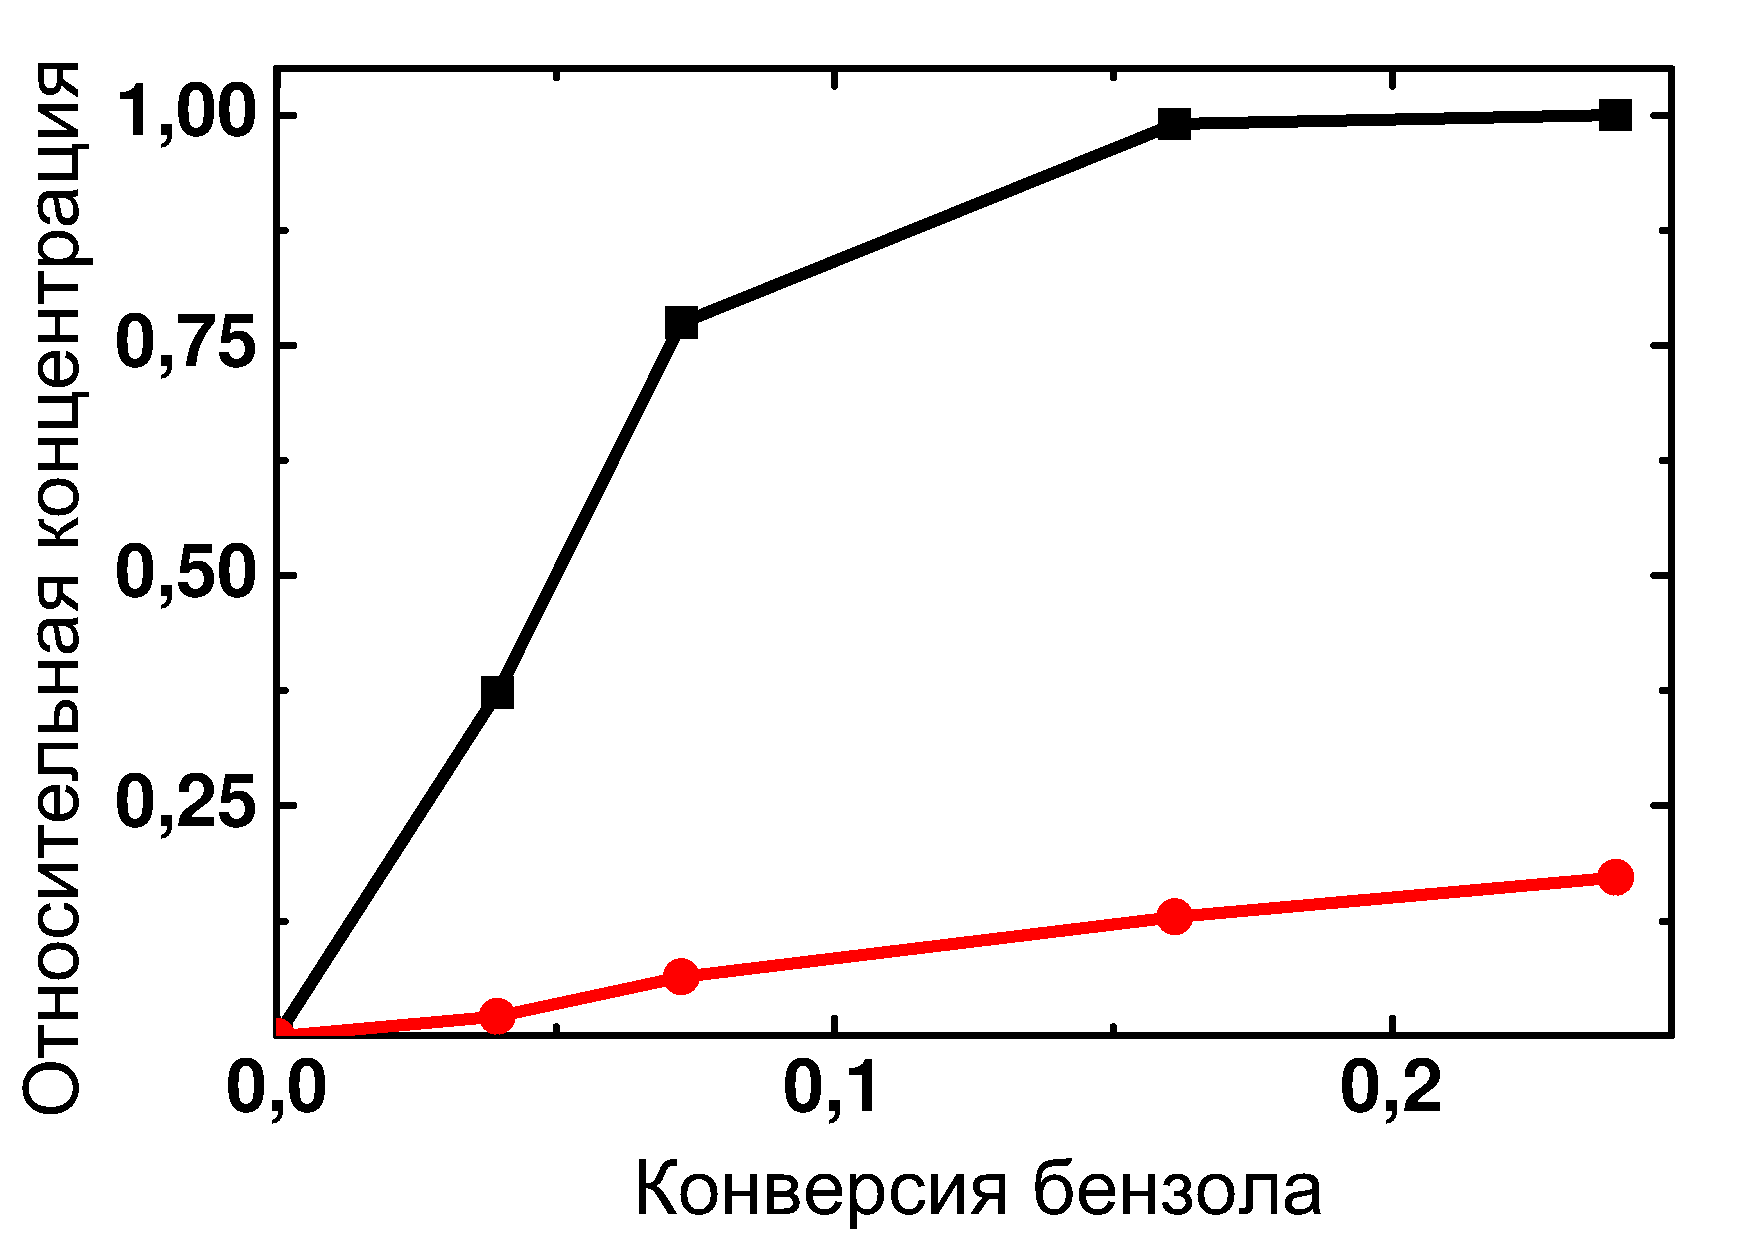
\includegraphics[width=0.6\linewidth]{prodXe+.pdf} \label{prodXe}}  
\caption{Кривые накопления фенильного радикала (чёрный) и фульвена (красный) в матрицах \subref{prodAr} аргона; \subref{prodKr} криптона; \subref{prodXe} ксенона} \label{tio}
\end{figure}
\newpage
Полученные из кривых накопления фенильного радикала и фульвена (рисунок~\ref{tio}) отношения концентраций (а значит, и отношения радиационно-химических выходов) фенильного радикала и фульвена представлены на рисунке \ref{rel}.  Это отношение сильно увеличивается при переходе от матриц аргона и криптона к матрице ксенона.
 
 \begin{figure}[h!]
\center{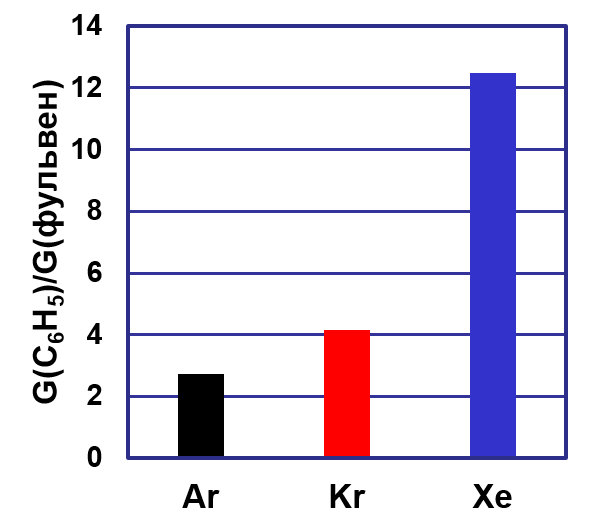
\includegraphics[width=0.5\linewidth]{rel1.png}}
\caption{Отношение выходов фенильного радикала и фульвена в различных матрицах}
\label{rel}
\end{figure}

Рост отношения выходов фенильного радикала и фульвена при переходе от матрицы аргона к матрице ксенона может быть связан как с увеличением выхода фенильного радикала, так и с уменьшением выхода фульвена в ряду Ar--Kr--Xe. Уменьшение радиационно-химического выхода фульвена в ряду Ar>Kr>Xe может быть объяснено увеличением эффективности интеркомбинационной конверсии. При переходе от матрицы аргона к матрице ксенона
понижается выход синглетных возбуждённых состояний бензола, из которых и образуется фульвен (см. раздел~\ref{photolysis}). Фенильный радикал образуется предположительно из высших триплетных возбуждённых состояний бензола. Эффективная интеркомбинационная конверсия повышает выход триплетных состояний бензола в матрицах криптона и ксенона, а значит радиационно-химический выход радикала C$_6$H$_5^\bullet$ должен расти в ряду Ar<Kr<Xe. Таким образом, увеличение выхода фенильного радикала и понижение выхода фульвена приводит к наблюдаемому изменению отношения их концентраций. 

Кроме того, необходимо отметить, что при рекомбинации возникающих при радиолизе электронов и катион-радикалов бензола образуются высшие триплетные и синглетные состояния бензола в отношении 3:1.  Этим обусловлено эффективное образование C$_6$H$_5^\bullet$ радикала при радиолизе бензола и его отсутствие при фотолизе, когда  высшие триплетные состояния практически не заселяются (см. разделы~\ref{radiolysis}, \ref{photolysis}). 


В ИК-спектрах облучённых образцов C$_6$H$_6$/Ng (Ng~= Ar, Kr, Xe) наблюдаются радиационно-индуцированные полосы поглощения в области 3330~см$^{-1}$ (см. рисунок~\ref{135_}), демонстрирующие ускорение роста с увеличением конверсии бензола (см. рисунок~\ref{135r}, каждая кривая пронормирована на собственное максимальное значение для возможности сравнения данных, полученных в различных матрицах). Такое поведение типично для продуктов вторичных радиационно-индуцированных реакций. Можно сделать предположение, что наборы полос, приведённые в таблицах~\ref{135}, \ref{1351}, соответствуют {\it цис}- и {\it транс}-изомерам гексадиен\nobreakdash-1,3\nobreakdash-ина\nobreakdash-5, так как образование данных продуктов описано при радиолизе и фотолизе бензола (см. раздел~\ref{radiolysis},~\ref{photolysis}). Кроме того, экспериментально полученные волновые числа удовлетворительно согласуются с данными квантово-химических расчётов. Многие полосы поглощения имеют сложную подструктуру, обусловленную наличием различных конформеров гексадиен\nobreakdash-1,3\nobreakdash-ина\nobreakdash-5, а так же <<сайтовым>> расщеплением (см. раздел \ref{isolation}).

 \begin{figure}[H]
\center{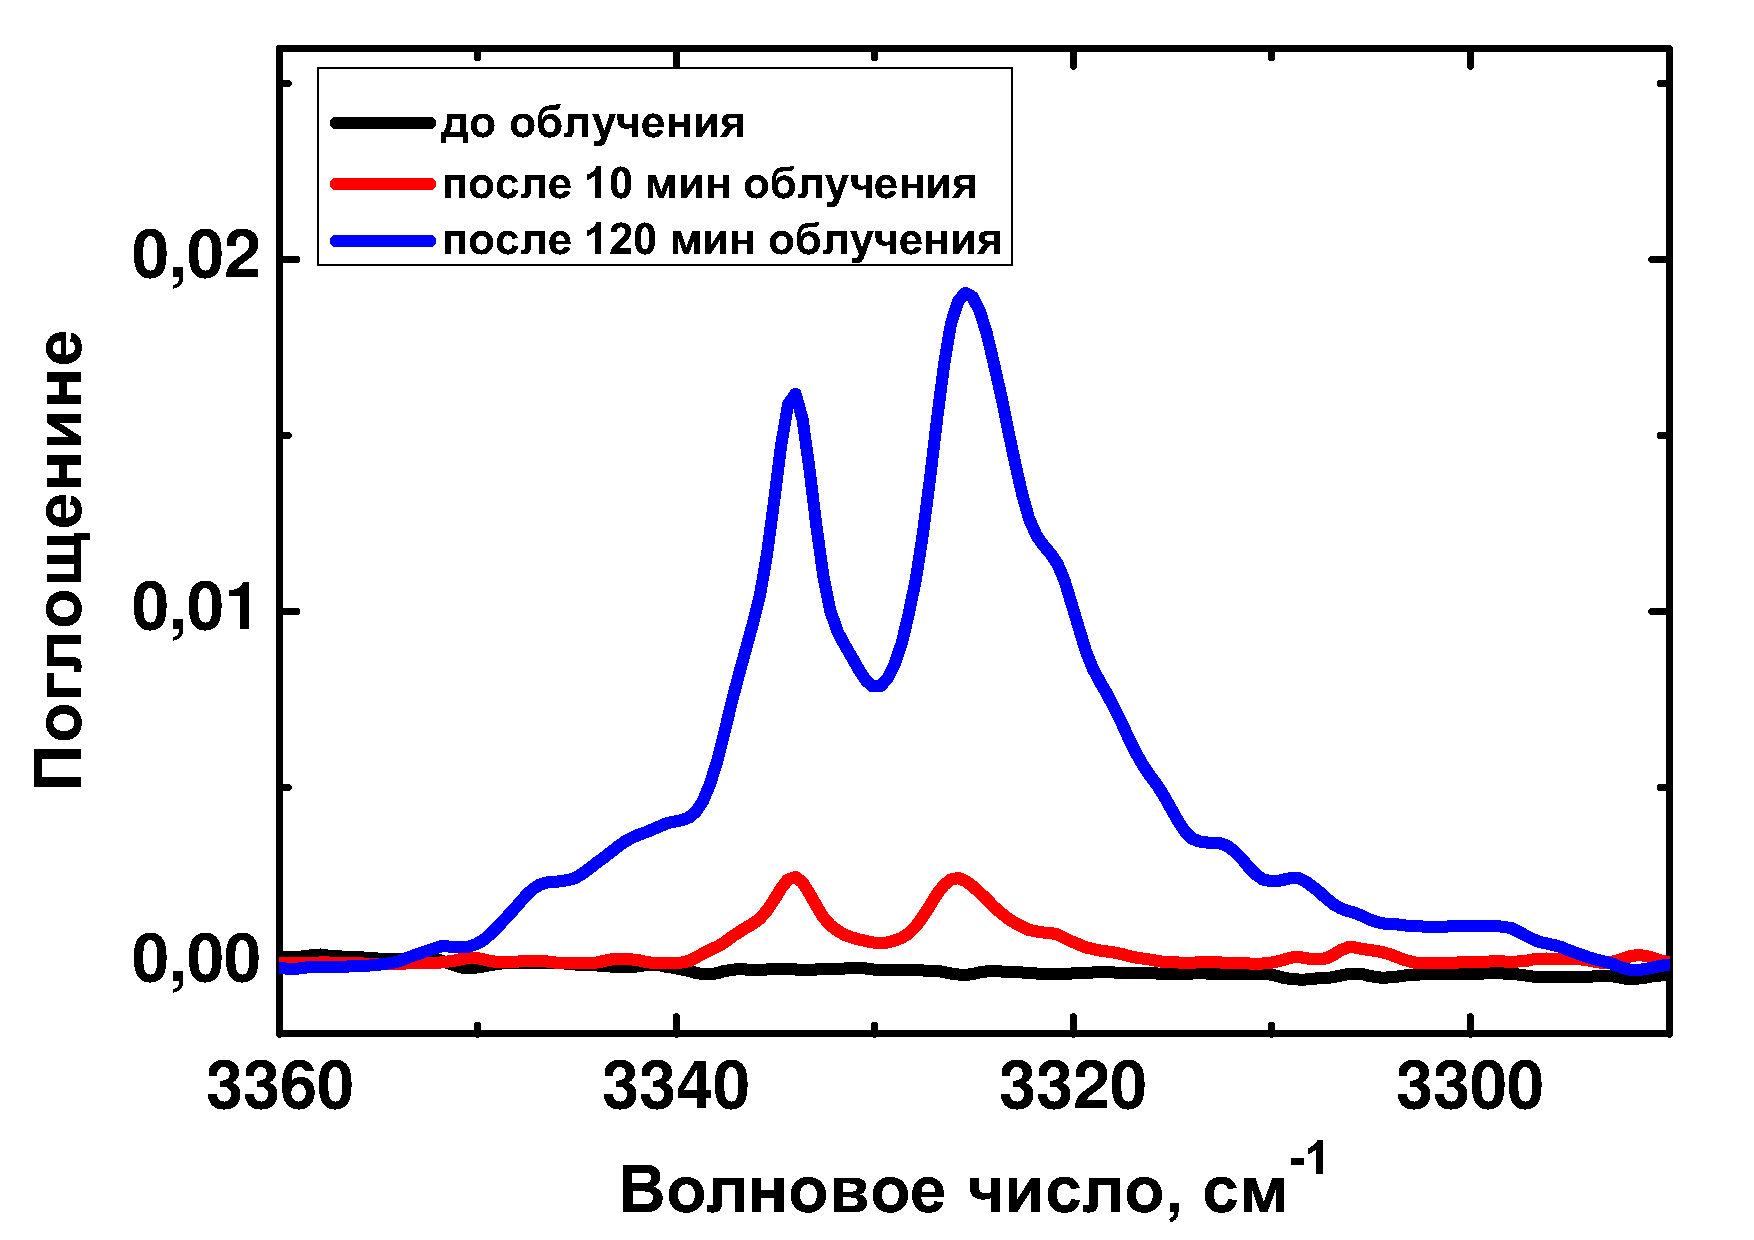
\includegraphics[width=0.9\linewidth]{135_.pdf}}
\caption{Фрагменты ИК-спектров образца C$_6$H$_6$/Ar, содержащие полосы поглощения гексадиен\nobreakdash-1,3\nobreakdash-ина\nobreakdash-5}
\label{135_}
\end{figure}

 \begin{figure}[H]
\center{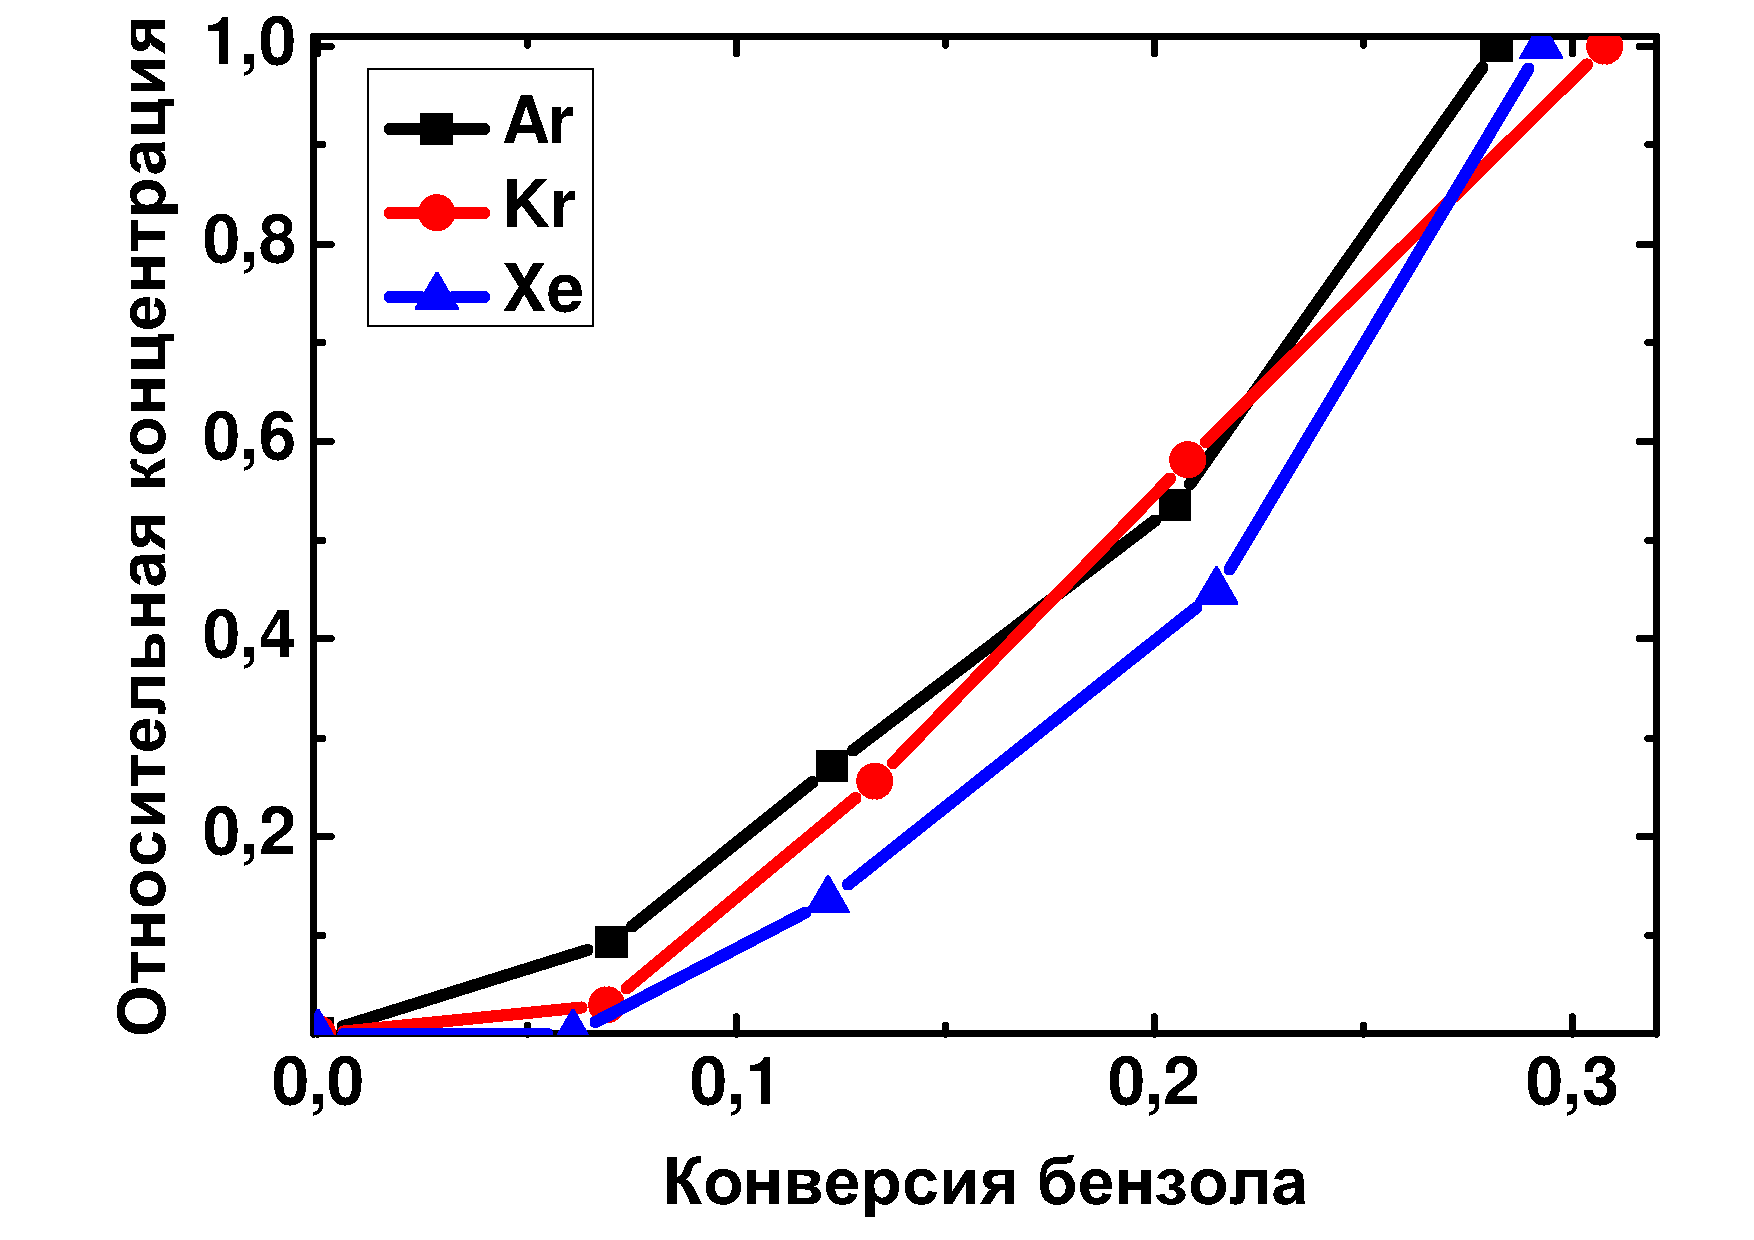
\includegraphics[width=0.9\linewidth]{135_s.pdf}}
\caption{Кривые накопления гексадиен\nobreakdash-1,3\nobreakdash-ина\nobreakdash-5 в различных матрицах}
\label{135r}
\end{figure}

\begin{table}[H]
\caption{Экспериментальные волновые числа~(Ar, Kr, Xe) и расчётные частоты~(PBE/L2\_3) колебаний {\it цис}-гексадиен\nobreakdash-1,3-ина-5~(см$^{-1}$)}
\label{135}
\begin{center}
\begin{tabular}{cccc}
Ar & Kr & Xe & Расчёт \\
\hline
620.9 & 619.7 & - & 620.8\\
759.2 & 758.7 & - & 765.2\\
913.5 & 912.6 & 909.8 & 910.2\\
1000.9 & 998.6 & 997.2 & 1001.68\\
1004.2 & 1002.6 & 1000.2 & 1006.78\\
3334.0 & 3333.9 & 3326.2 & 3407.3\\
3336.9 &  & \\
\end{tabular}
\end{center}
\end{table}

\begin{table}[H]
\caption{Экспериментальные волновые числа~(Ar, Kr, Xe) и расчётные частоты~(PBE/L2\_3) колебаний {\it транс}-гексадиен\nobreakdash-1,3-ина-5~(см$^{-1}$)}
\label{1351}
\begin{center}
\begin{tabular}{cccc}
Ar & Kr & Xe & Расчёт \\
\hline
630.9 & 629.8 & 626.4 & 629.3\\
894.3 & 893.3 & 892.1 & 897.1\\
948.7 & 947.1 & 946.1 & 946.9\\
3325.7 & 3313.4 & 3315.2 & 3408.9\\
 & 3325.9 & 3312.4 & \\
\end{tabular}
\end{center}
\end{table}

Известно, что гексадиен\nobreakdash-1,3\nobreakdash-ин\nobreakdash-5 может образовываться из фульвена при фотолизе. В матрицах криптона и ксенона при конверсиях бензола больше 0.15 образование фульвена замедляется, следовательно, логично предположить, что и в данном случае гексадиен\nobreakdash-1,3\nobreakdash-ин\nobreakdash-5 образуется из фульвена. В матрице аргона кривая накопления фульвена практически линейна, при этом некоторые количества гексадиен\nobreakdash-1,3\nobreakdash-ина\nobreakdash-5 образуются уже при малых конверсиях бензола. Это свидетельствует о наличии альтернативного <<одностадийного>> механизма образования гексадиен\nobreakdash-1,3\nobreakdash-ина\nobreakdash-5 в матрице аргона. Молекула фульвена, образующаяся в возбуждённом состоянии, не релаксирует в основное состояние, а сразу же претерпевает изомеризацию. Вклад данного механизма наиболее значителен именно в матрице аргона, так как в случае более поляризуемых матриц (Kr, Xe)  релаксация образующегося фульвена протекает значительно эффективнее.
 
Фотолиз облучённых образцов C$_6$H$_6$/Ng в видимой области и ближнем УФ-диапазоне не приводит к значительным изменениям в ИК-спектре ни в одной из матриц. 

\subsection{Радиолиз бензола-$d_6$}

В ИК-спектрах осаждённых образцов C$_6$D$_6$/Ng присутствуют полосы поглощения, соответствующие дейтерированному бензолу. Отнесение основано на литературных спектроскопических данных для газовой фазы с учётом разумных матричных сдвигов~\cite{Shimanouchi}. 
Типичный вид спектра осаждённой смеси представлен на рисунке~\ref{Ar_d6}. 

 \begin{figure}[H]
\center{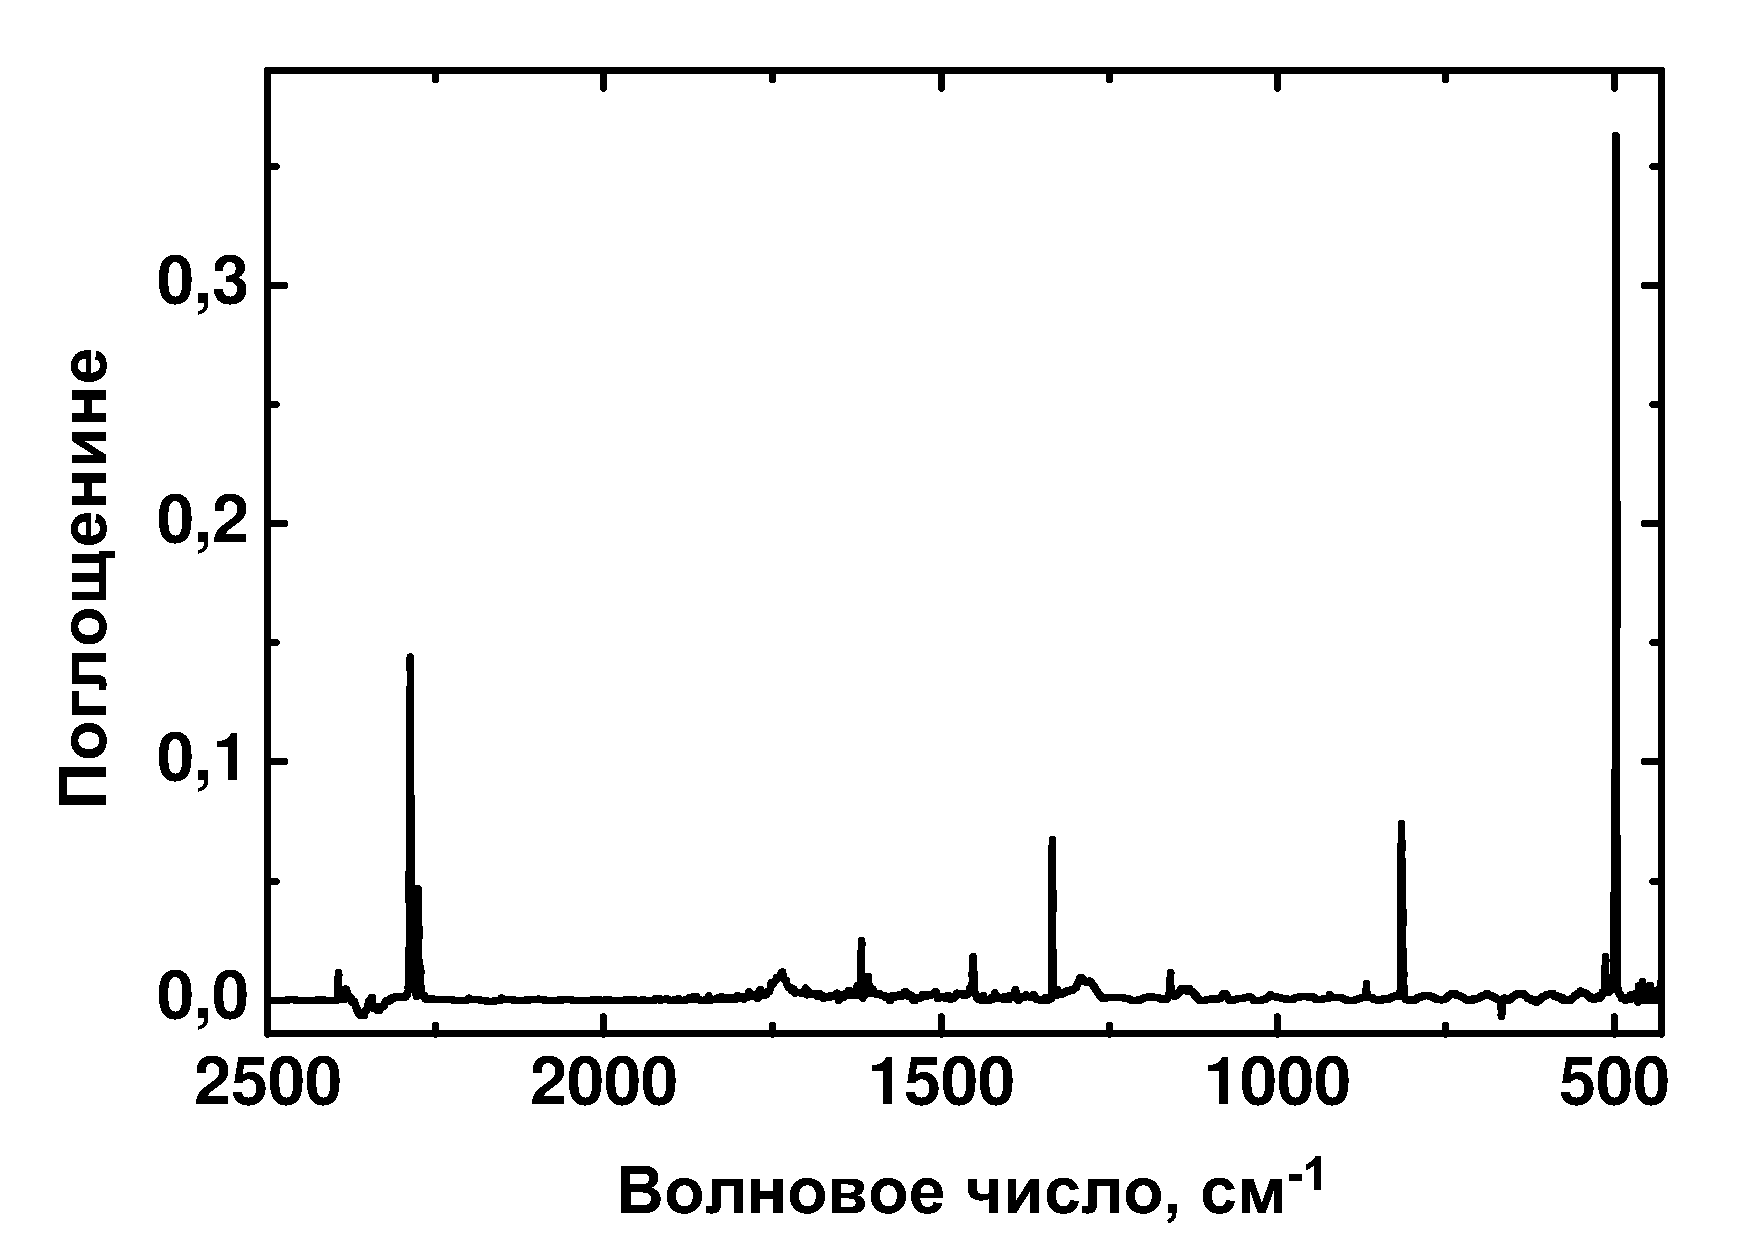
\includegraphics[width=0.9\linewidth]{is_d.pdf}}
\caption{ИК-спектр осаждённой смеси C$_6$D$_6$/Ar 1:1000}
\label{Ar_d6}
\end{figure}


В результате радиолиза осаждённых образцов C$_6$D$_6$/Ng (Ng~= Ar, Kr, Xe) дейтерированный бензол разлагается довольно эффективно. На рисунке~\ref{comp} представлены кривые расходования C$_6$D$_6$ в различных матрицах, для сравнения приведены кривые расходования C$_6$H$_6$. Из данных зависимостей видно, что бензол\nobreakdash-$d_6$ расходуется немного медленнее, чем недейтерированный бензол в соответствующих матрицах. Закономерно, что радиационно-химические выходы расходования бензола-$d_6$, определённые из начальных участков кривых аналогично случаю недейтерированного бензола по уравнению \ref{yee}, составили: для матрицы аргона $G$(--C$_6$D$_6$)~= 1.5~молек./100~эВ, для матриц криптона и ксенона    $G$(--C$_6$D$_6$)~= 0.3~молек./100~эВ.


 \begin{figure}[H]
\center{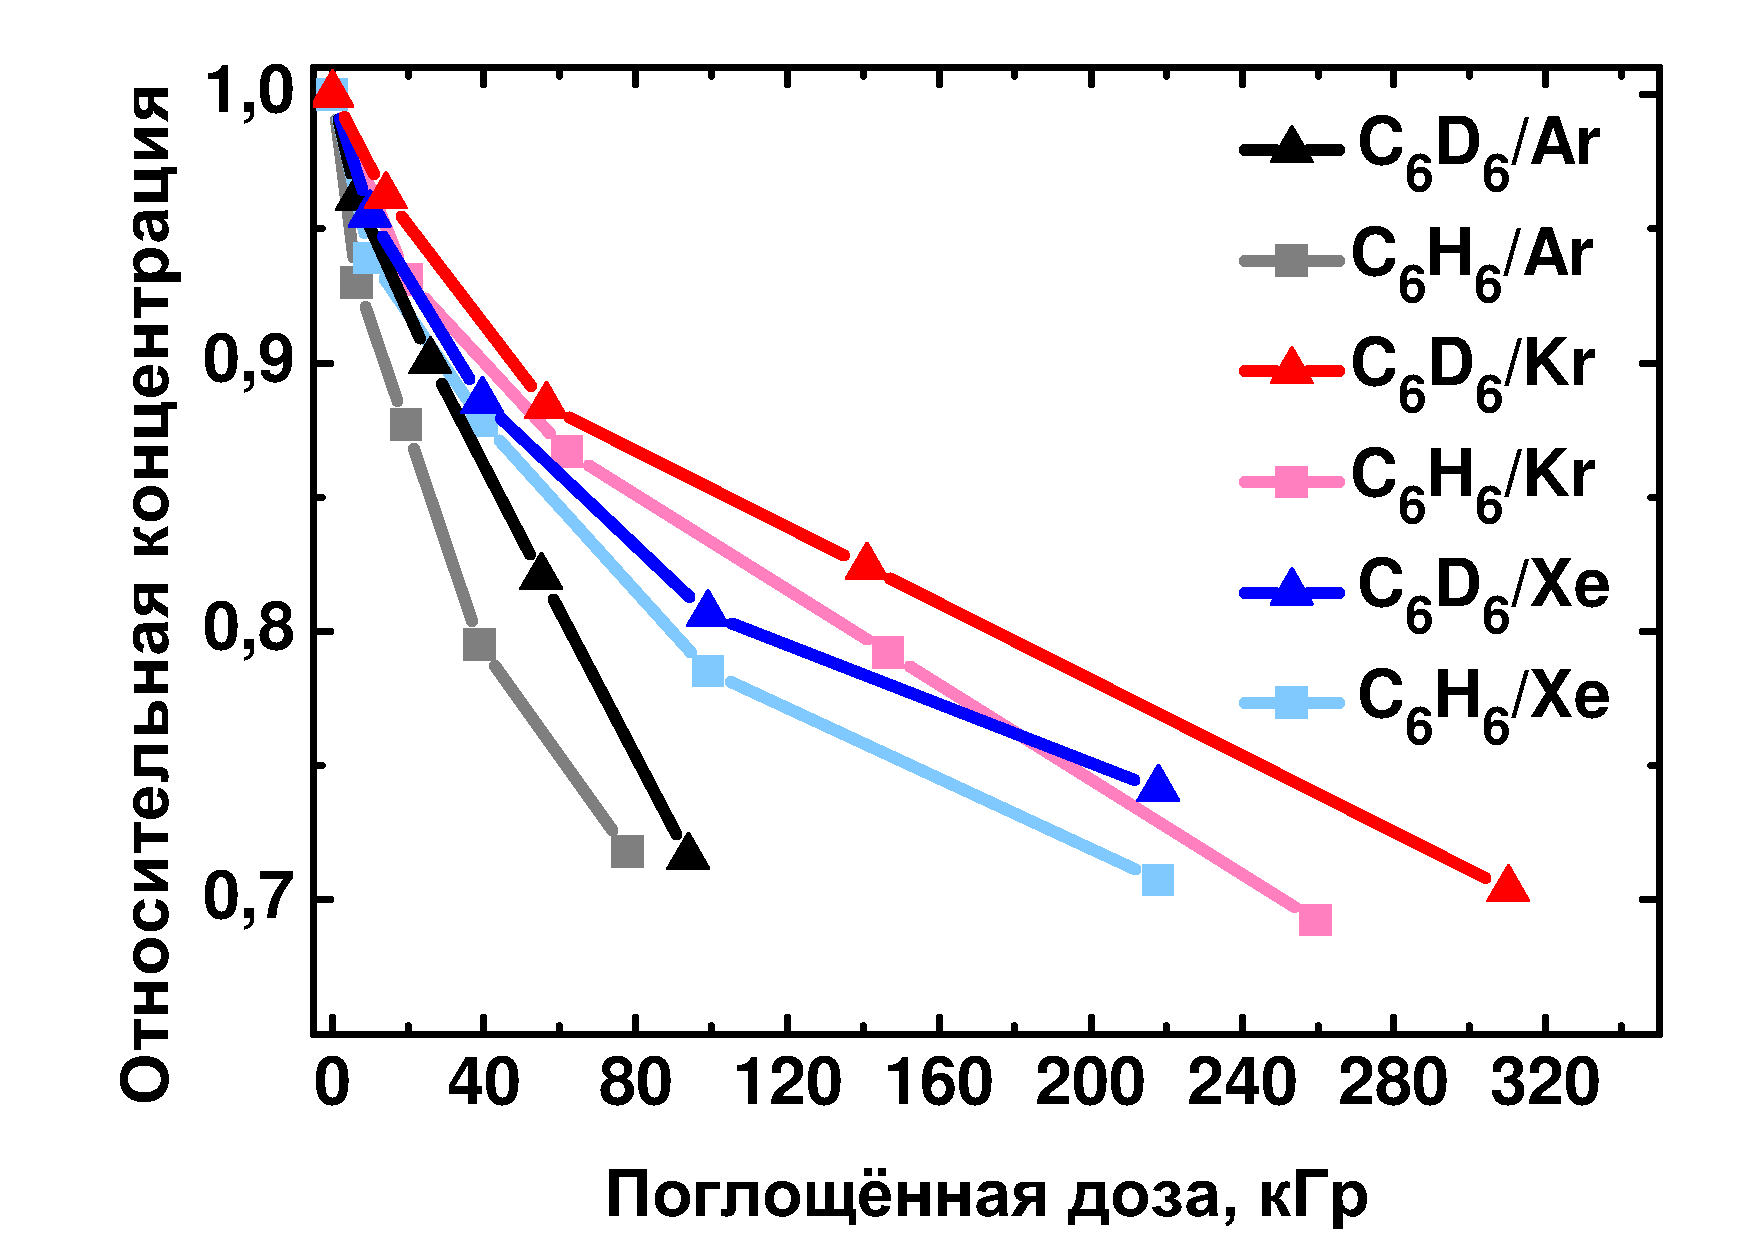
\includegraphics[width=0.9\linewidth]{comp_dose_2col.pdf}}
\caption{Зависимости относительной концентрации бензола и бензола-$d_6$ от поглощённой дозы}
\label{comp}
\end{figure}

После облучения образцов C$_6$D$_6$/Ng в ИК-спектрах появляются дополнительные полосы поглощения. Во всех матрицах наблюдается образование радикала~C$_6$D$_5^\bullet$ (см. таблицу~\ref{C6D5}), отнесение основано на литературных данных~\cite{Friderichsen2001}. Спектроскопические характеристики фульвена-$d_6$ в литературе отсутствуют, однако логично предположить образование фульвена-$d_6$ при радиолизе смесей C$_6$D$_6$/Ng, аналогично экспериментам с образцами С$_6$Н$_6$/Ng. Действительно, волновые числа радиационно-индуцированных полос поглощения хорошо согласуются с данными квантово-химических расчётов (см. таблицу~\ref{fd6}).

 \begin{table}[H]
\caption{Волновые числа колебаний радикала C$_6$D$_5^\bullet$~(см$^{-1}$) в~различных матрицах}
\label{C6D5}
\begin{center}
\begin{tabular}{ccc}
Ar & Kr & Xe \\
\hline
517.7 & 517.2 & 516.1 \\
- & - & 587.8 \\
802.8 & 801.2 & 799.9 \\
806.0 & 804.5 & 802.7 \\
- & - & 1308.8 \\
- & 1312.6 & 1311.9 \\
\end{tabular}
\end{center}
\end{table}


 \begin{table}[H]
\caption{Экспериментальные волновые числа~(Ar, Kr, Xe) и расчётные частоты~(PBE/L2\_3) колебаний фульвена-$d_6$~(см$^{-1}$)}
\label{fd6}
\begin{center}
\begin{tabular}{cccc}
Ar & Kr & Xe & Расчёт\\
\hline
487.8 & 487.2 & 486.7 & 484.6\\
489.2 & 488.9 & 488.2 & \\
773.1 & 772.0 & 771.1 & 777.2 \\
1447.0 & - & - & 1455.4\\
\end{tabular}
\end{center}
\end{table}

Кривые накопления основных продуктов радиолиза бензола-$d_6$ в различных матрицах представлены на рисунке \ref{tio-d}. Для их получения использованы следующие молярные коэффициенты поглощения: 18.7~км/моль для полосы поглощения, соответствующей внеплоскостным колебаниям в группе CD$_2$ фульвена (773.1~см$^{-1}$ в аргоне), 29.3~км/моль для полосы поглощения, соответствующей внеплоскостным колебаниям связи C--H фенильного радикала (517.7~см$^{-1}$ в аргоне), оба коэффициента получены в результате квантово-химических расчётов (для C$_6$D$_5^\bullet$ из \cite{Friderichsen2001}). Накопление C$_6$D$_5^\bullet$ и фульвена-$d_6$ протекает, в целом, аналогично случаю недейтерированного бензола, однако в случае C$_6$D$_6$ относительная концентрация фульвена-$d_6$  несколько выше. Начальные участки кривых накопления линейны, поэтому можно сделать вывод о том, что оба продукта являются первичными в матрицах аргона и криптона; в матрице ксенона C$_6$D$_5^\bullet$ также является первичным продуктом, а фульвена образуются только незначительные количества.

\begin{figure}[H]  
\vspace{-4ex} \centering \subfigure[]{
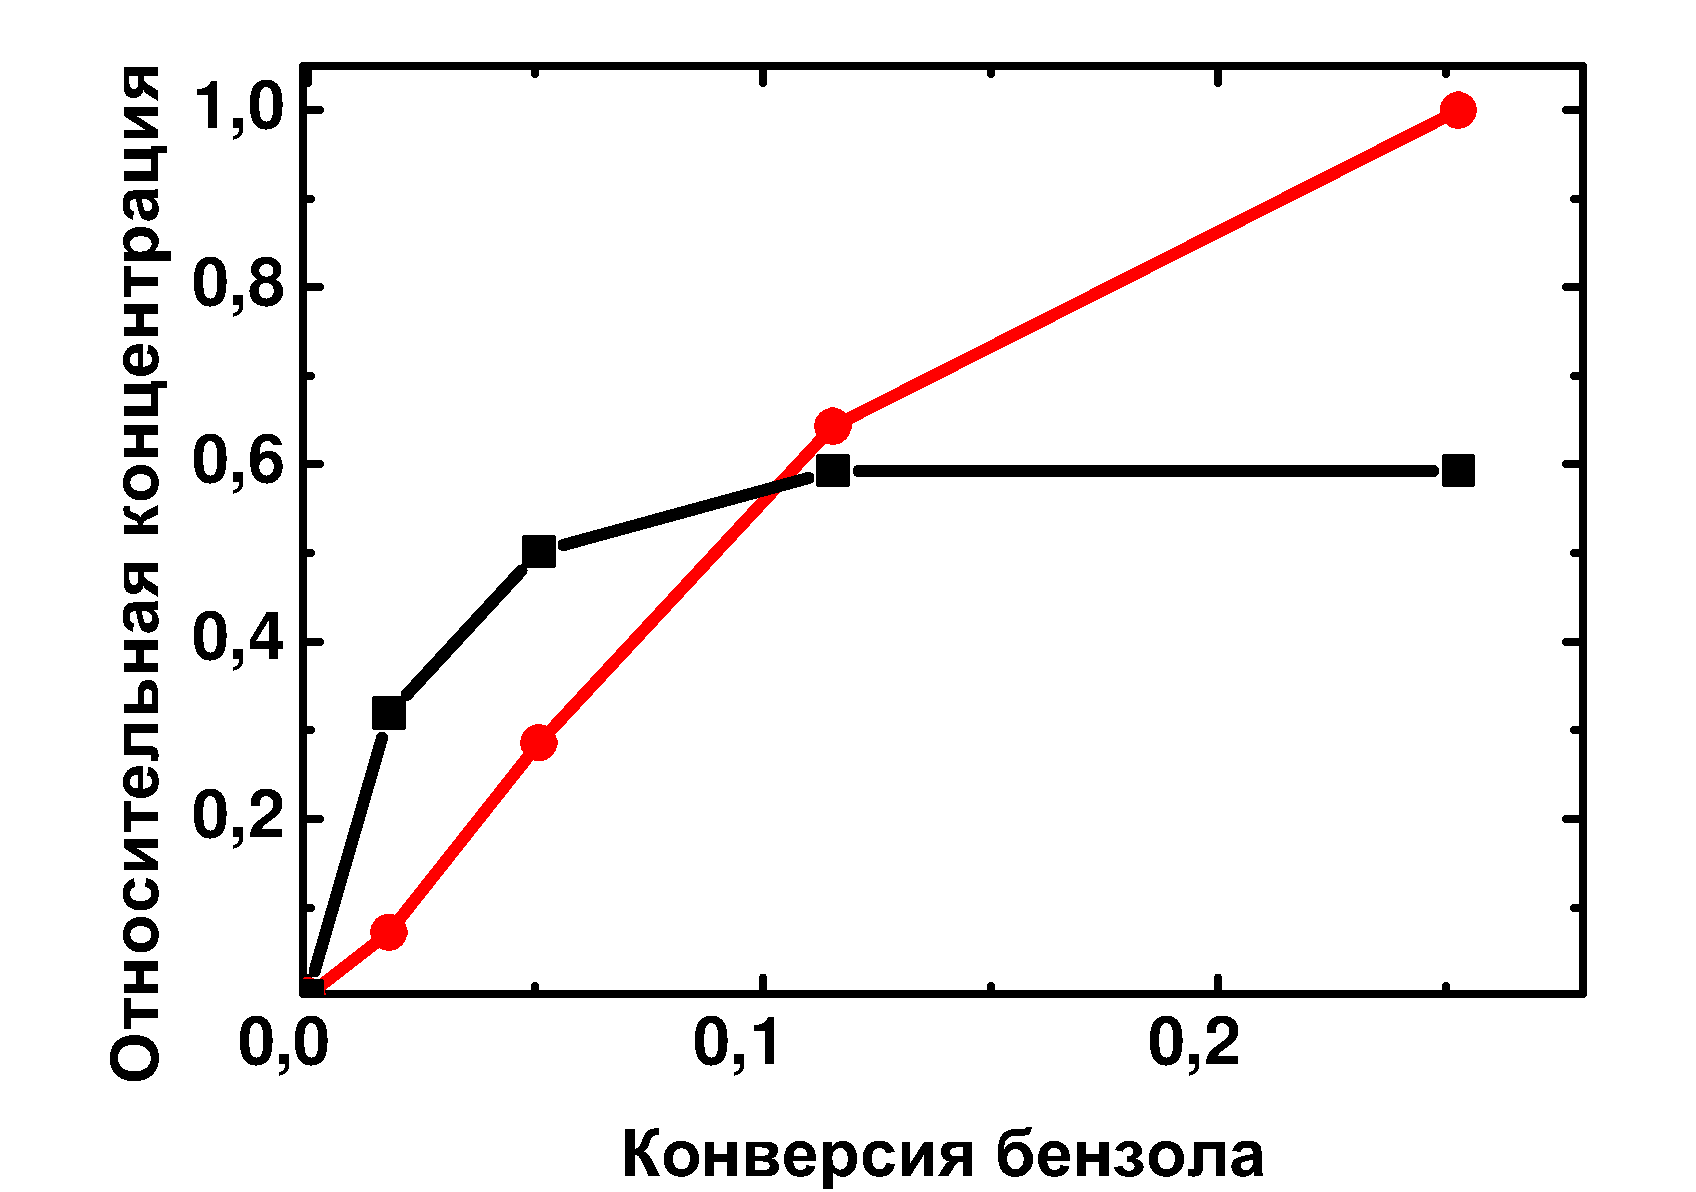
\includegraphics[width=0.6\linewidth]{prod_Ar_d6_xxxx.pdf} \label{prod_Ar_d6}}  
\hspace{4ex}
\subfigure[]{
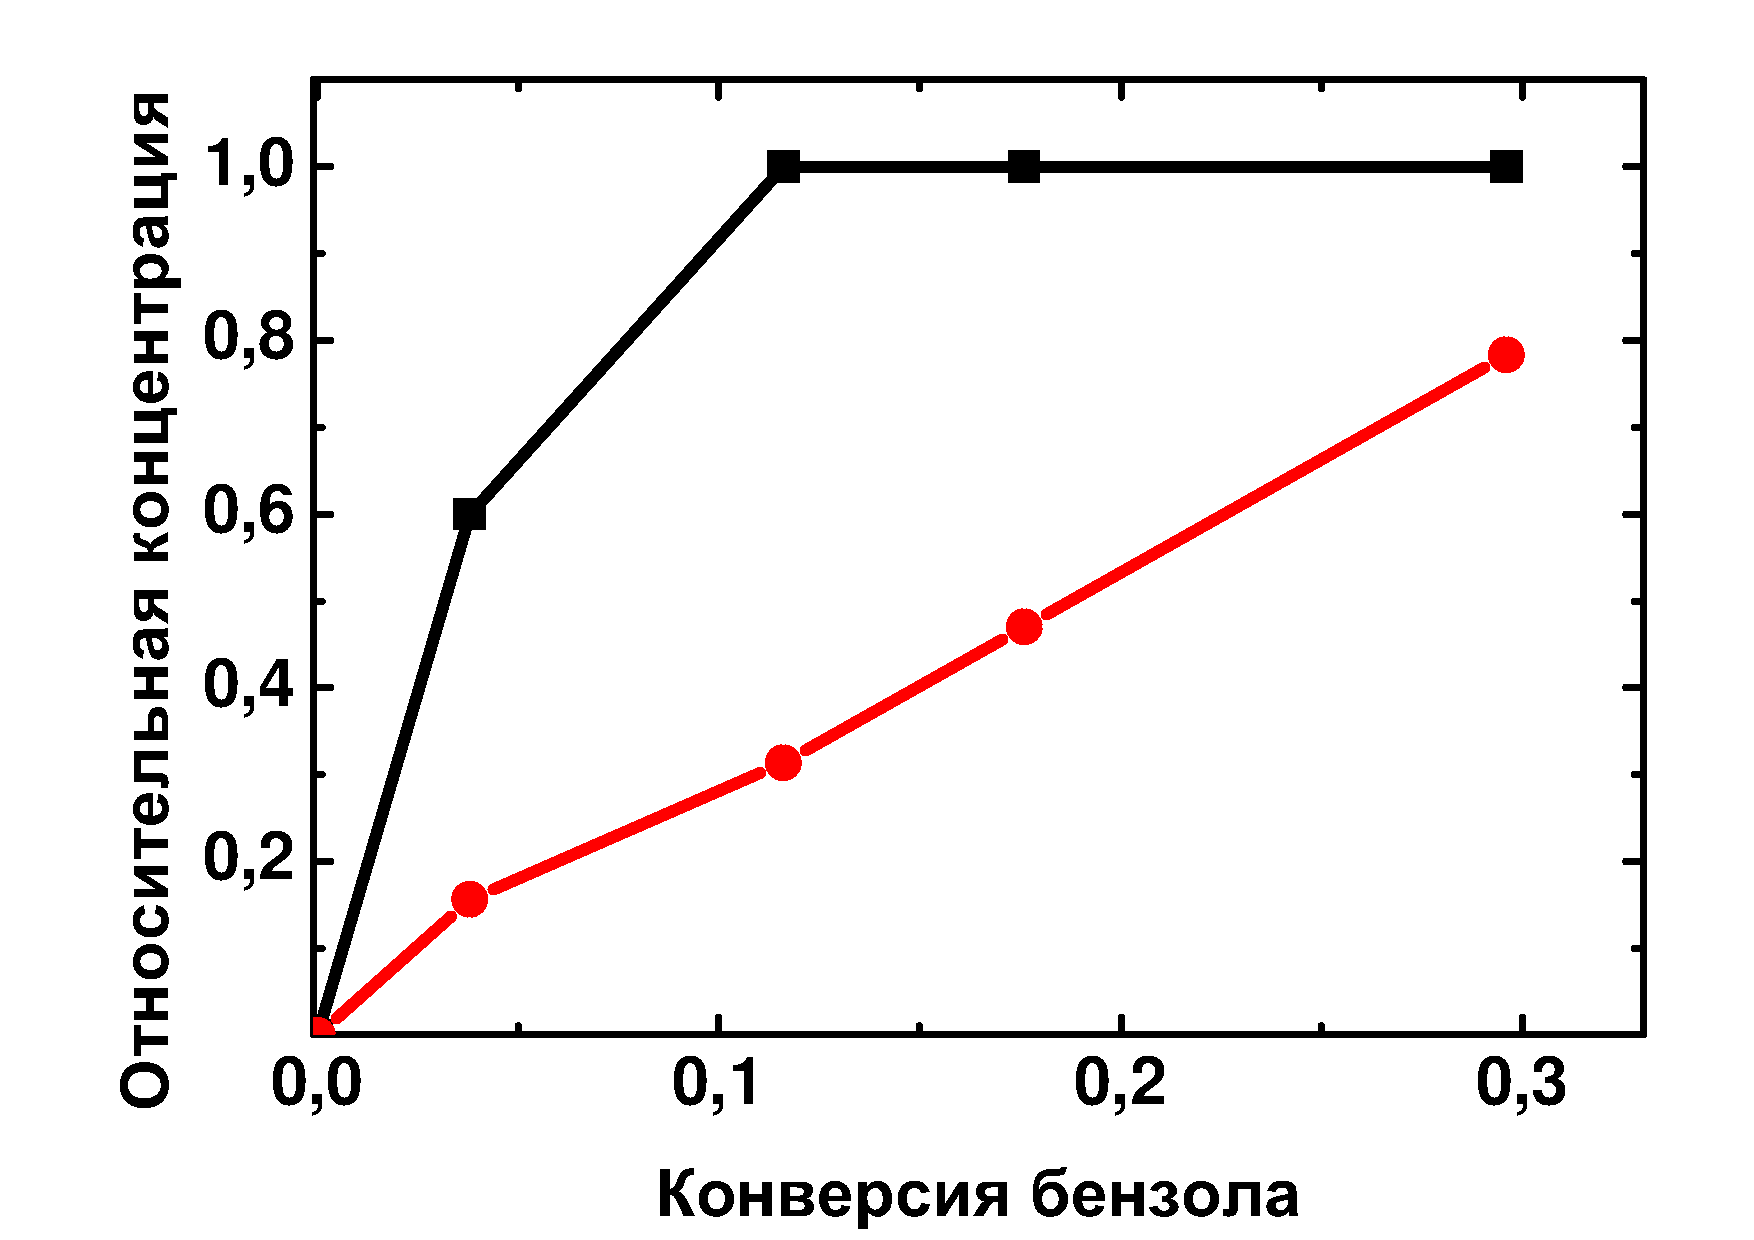
\includegraphics[width=0.6\linewidth]{prod_Kr_d6_xxxx.pdf} \label{prod_Kr_d6}}
\hspace{4ex}
\subfigure[]{
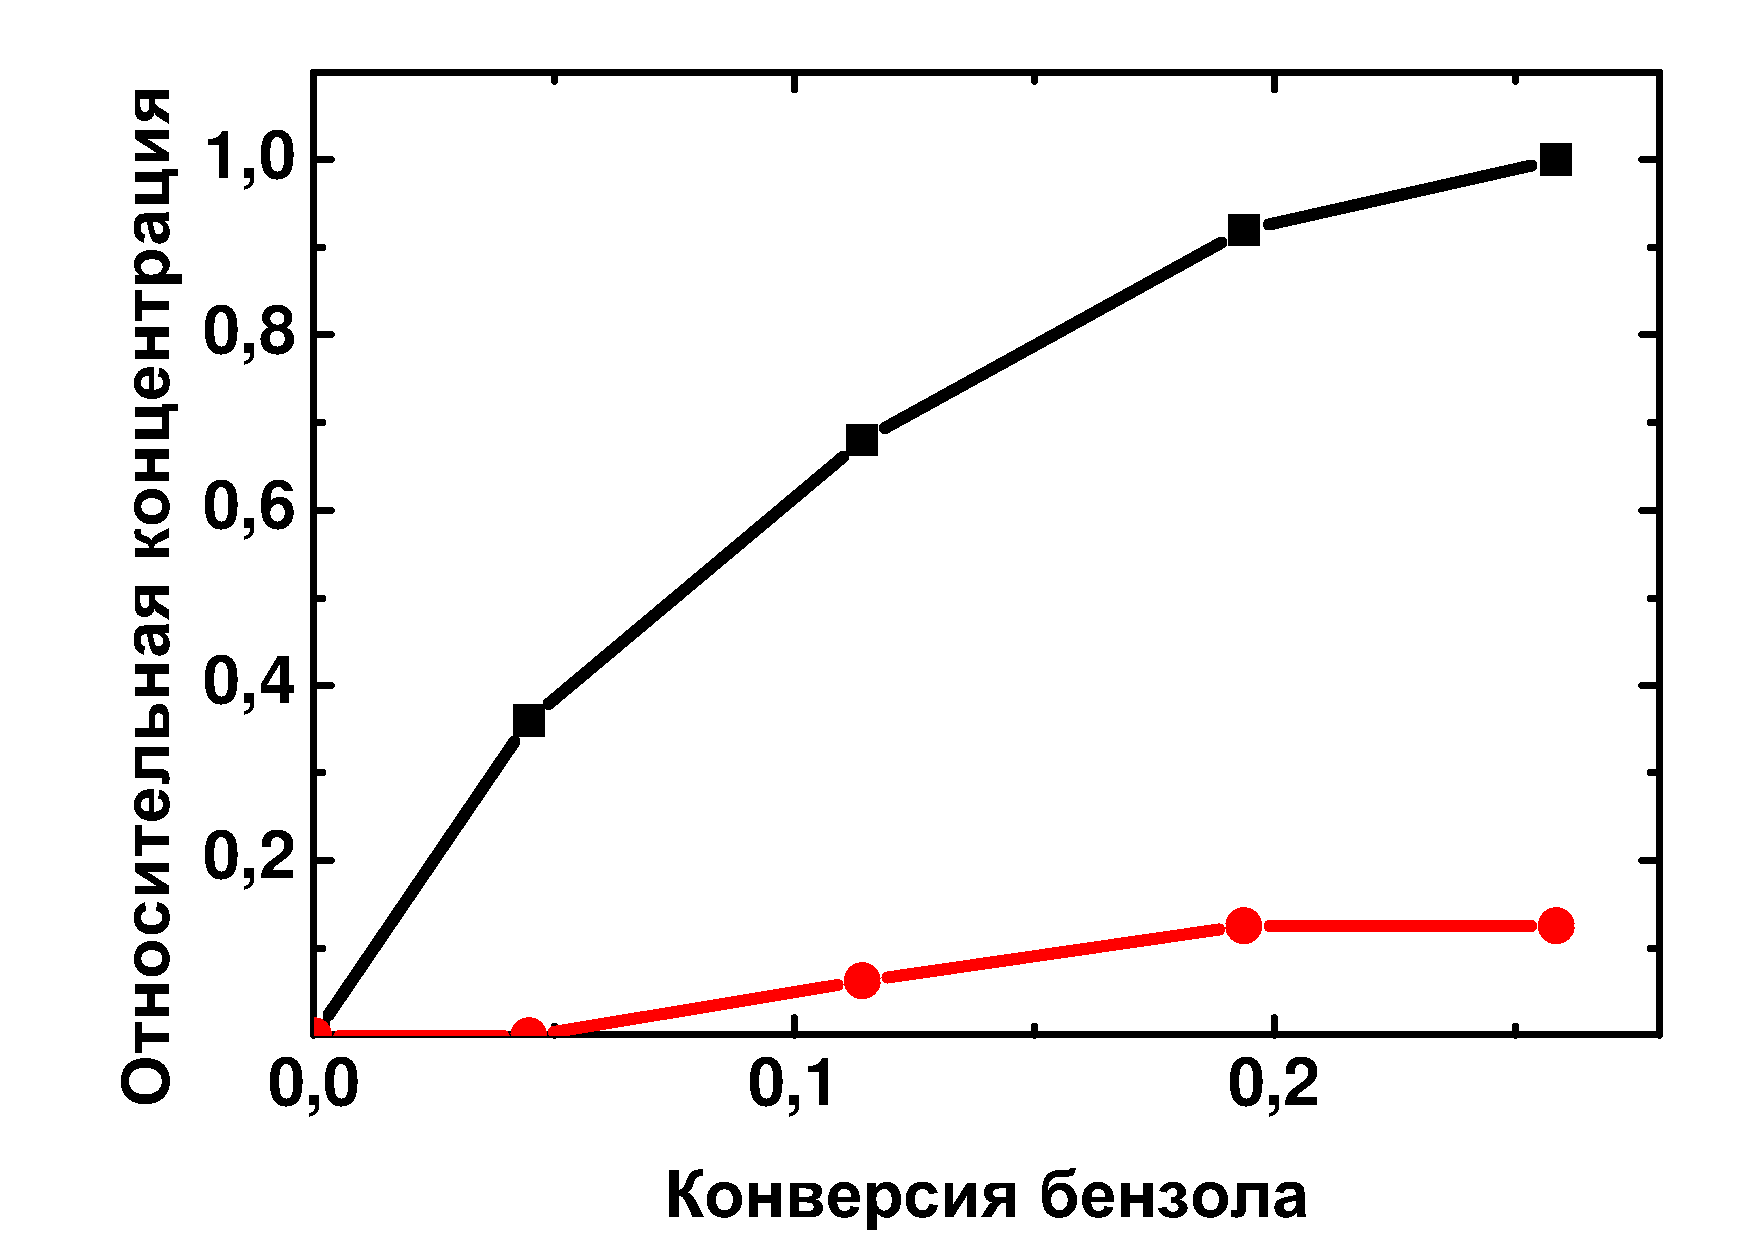
\includegraphics[width=0.6\linewidth]{prod_Xe_d6_xxxx.pdf} \label{prod_Xe_d6}}  
\caption{Кривые накопления фенильного радикала C$_6$D$_5^\bullet$ (чёрный) и фульвена-$d_6$ (красный) в матрицах \subref{prod_Ar_d6}~аргона; \subref{prod_Kr_d6}~криптона; \subref{prod_Xe_d6}~ксенона} \label{tio-d}
\end{figure}

 Отношение интенсивностей радикала C$_6$D$_5^\bullet$ и фульвена-$d_6$ увеличивается в ряду Ar<Kr<Xe. Причины этой закономерности аналогичны случаю недейтерированного бензола.

После облучения бензола-$d_6$ в матрицах аргона и криптона присутствуют полосы поглощения сольватированного дейтрона Ng$_2$D$^+$ (643.2~см$^{-1}$ для Ar и 605.8~см$^{-1}$ для Kr). В случае  ксенона не наблюдается образования значительных количеств Xe$_2$D$^+$. Его полоса поглощения имеет волновое число 517~см$^{-1}$, то есть накладывается на полосу поглощения радикала C$_6$D$_5^\bullet$, однако интенсивность этой полосы при фотолизе в УФ-диапазоне не уменьшается, а значит она соответствует только радикалу, но не  сольватированному дейтрону (см. раздел~\ref{isolation}).

 Во всех матрицах при радиолизе бензола-$d_6$ наблюдается появление интенсивных полос поглощения в области 2600~см$^{-1}$. Данные полосы демонстрируют ускорение роста с увеличением конверсии бензола, что характерно для вторичных продуктов радиационно-индуцированных реакций.  Волновые числа этих полос поглощения примерно в $\sqrt{2}$~ раз меньше, чем волновые числа полос поглощения валентных C--H колебаний при тройной связи гексадиен\nobreakdash-1-ина\nobreakdash-5 (3300~см$^{-1}$).  Можно предположить, что в результате радиационно-индуцированных превращений бензола образуется гексадиен\nobreakdash-1-ин\nobreakdash-5-$d_6$ (см.~таблицу~\ref{135d}), а полосы с волновыми числами около 2600~см$^{-1}$ соответствуют валентным колебаниям C\nobreakdash--D связи. Однако определить, {\it цис}- или {\it транс}-изомер преимущественно стабилизируется в матрицах, невозможно по нашим данным, так как изомеры имеют близкие частоты колебаний.
 
 \begin{table}[H]
\caption{Экспериментальные волновые числа~(Ar, Kr, Xe) и расчётные частоты~(PBE/L2\_3) колебаний {\it цис}- и {\it транс}-гексадиен\nobreakdash-1,3-ина-5~(см$^{-1}$)}
\label{135d}
\begin{center}
\begin{tabular}{ccccc}
Ar & Kr & Xe & Расчёт для  & Расчёт для\\
&&&{\it цис}-изомера&{\it транс}-изомера\\
\hline
493.4 & - & - & 491.9 & 490.7\\
715.2 & 713.8 & 711.9 & 712.7 & 704.27\\
2602.8 & 2595.9 & 2588.2 & 2640.3 & 2643.0\\
 & 2599.2 &  &  & \\
\end{tabular}
\end{center}
\end{table}

В литературе отсутствуют данные о спектроскопических характеристиках дейтерированных изомеров бензола. Для более точной идентификации продуктов радиолиза бензола-$d_6$ в матрицах был проведён фотолиз осаждённой смеси~C$_6$D$_6$/Ar.
В результате фотолиза ртутной лампой среднего давления (содержит излучение с длиной волны 254~нм) образуются изомеры бензола: фульвен\nobreakdash-$d_6$, бензвален\nobreakdash-$d_6$ и бензол Дьюара\nobreakdash-$d_6$ (см. рисунок~\ref{diff}). Экспериментально полученные волновые числа удовлетворительно соотносятся с данными квантово-химических расчётов (см.~таблицы~\ref{benz_fr}, \ref{Dewar_fr}).  Полученный результат согласуется с литературными данными по фотолизу C$_6$H$_6$ в матрице аргона (см.~раздел~\ref{photolysis}).  

 \begin{figure}[H]
\center{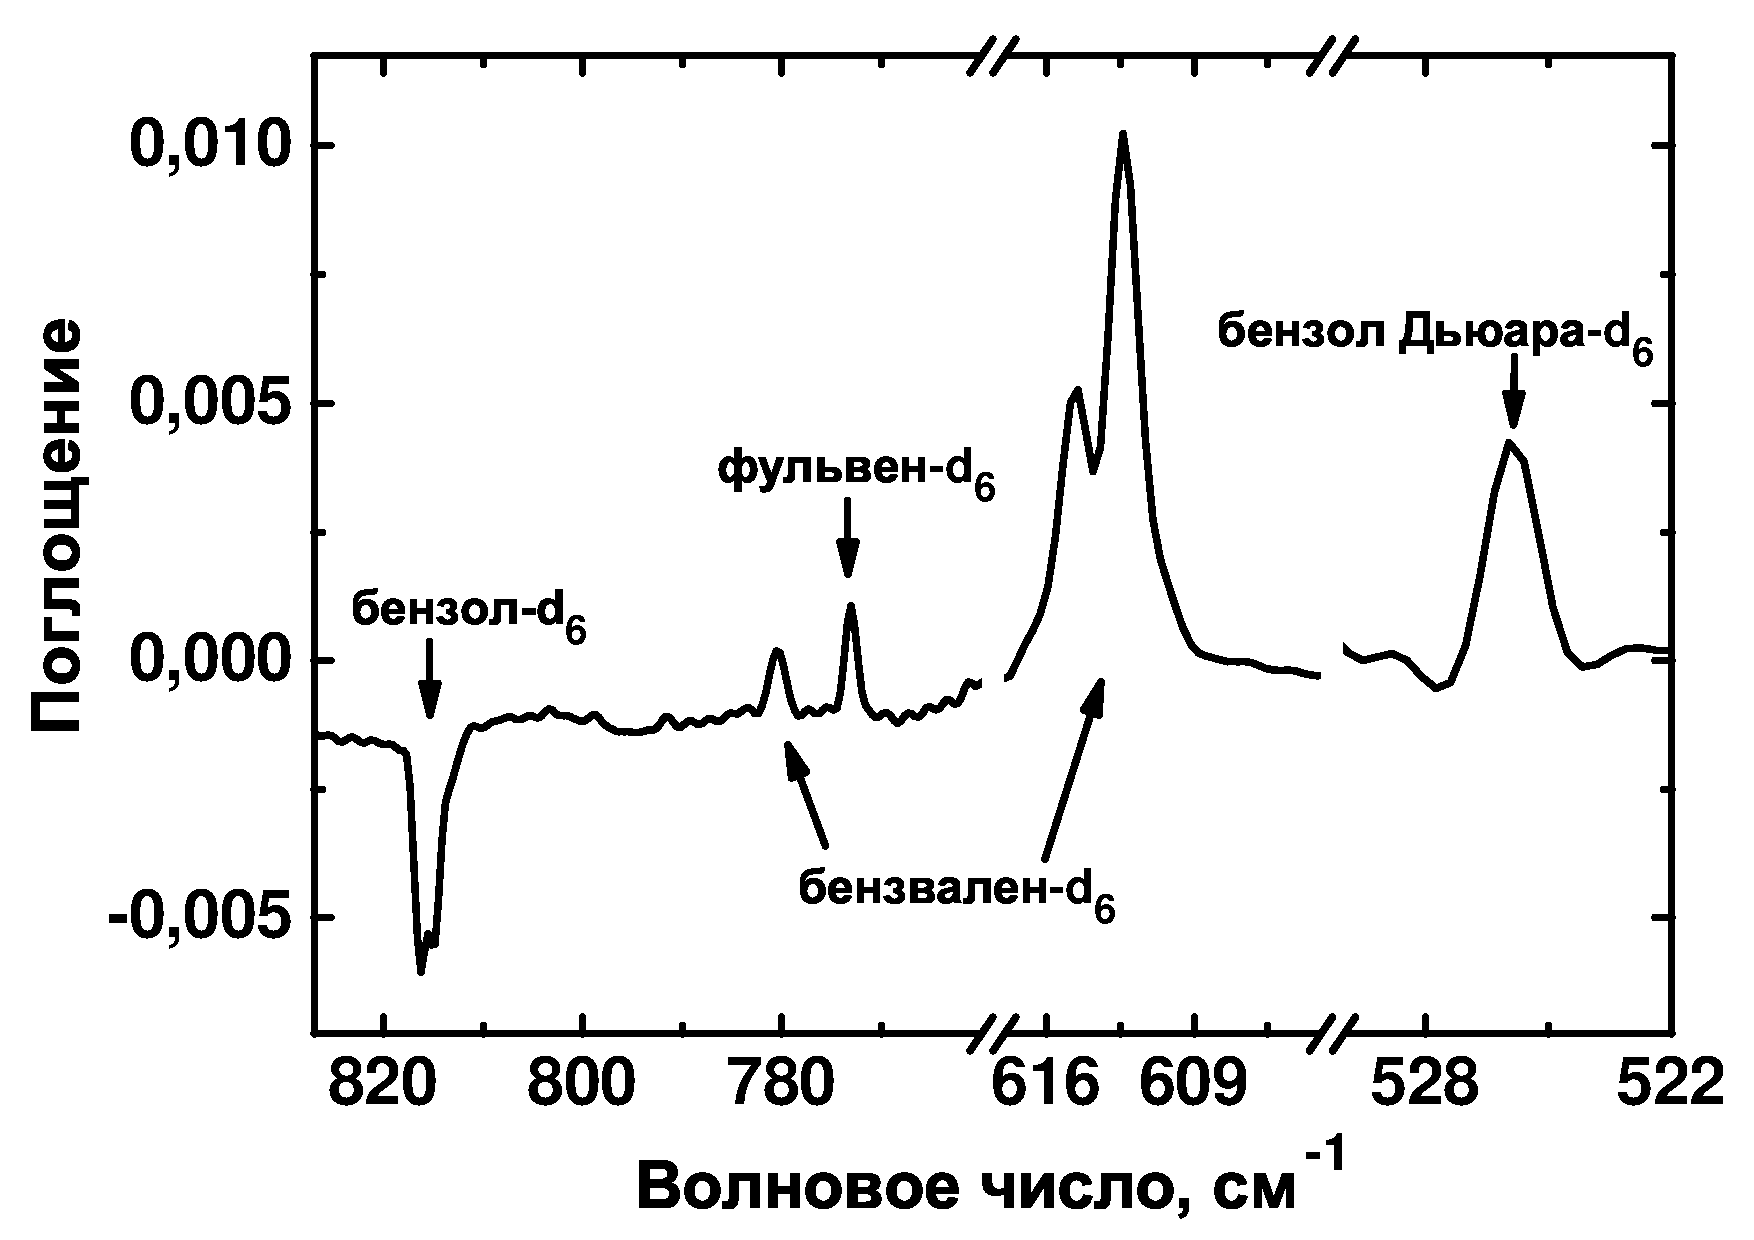
\includegraphics[width=\linewidth]{ph_sp.pdf}}
\caption{Разностный спектр фотолизованого и осаждённого образцов C$_6$D$_6$/Ar}
\label{diff}
\end{figure}

 \begin{table}[H]
\caption{Экспериментальные волновые числа (Ar) и расчётные частоты~(PBE/L2\_3) колебаний бензвалена-$d_6$~(см$^{-1}$)}
\label{benz_fr}
\begin{center}
\begin{tabular}{cc}
Ar &  Расчёт \\
\hline
612.4 & 608.5\\
614.7 & \\
640.6 & 640.7\\
642.7 & \\
780.4 & 770.5\\
\end{tabular}
\end{center}
\end{table}

 \begin{table}[H]
\caption{Экспериментальные волновые числа (Ar) и расчётные частоты~(PBE/L2\_3) колебаний бензола Дьюара-$d_6$~(см$^{-1}$)}
\label{Dewar_fr}
\begin{center}
\begin{tabular}{cc}
Ar &  Расчёт \\
\hline
519.6 & 524.4\\
525.9 & \\
631.7 & 635.3\\
654.8 & 650.2\\
657.6 & \\
733.4 & 735.3\\
\end{tabular}
\end{center}
\end{table}


Итак, проведём сравнение процессов протекающих при радиолизе и фотолизе бензола в матрицах. 
Процессы, происходящие при радиолизе бензола в матрицах можно описать следующими уравнениями:
\vspace{-2ex}
\begin{equation}\label{eq1_}
\mathrm{ 
Ng \leadsto Ng^{+\bullet}, e^-, Ng^*}
\end{equation}
\begin{equation}\label{eq2_}
\mathrm{
Ng^{+\bullet} + C_6H_6  \to (C_6H_6^{+\bullet})^* + Ng}
\end{equation}
\begin{equation}\label{eq3_}
\mathrm{
Ng^* + C_6H_6   \to C_6H_6^*  + Ng}
\end{equation}
\begin{equation}\label{eq4_}
\mathrm{
(C_6H_6^{+\bullet})^*  \to C_6H_6^{+\bullet} }
\end{equation}
\begin{equation}\label{eq6_}
\mathrm{
C_6H_6^{+\bullet}   + e^- \to C_6H_6^{**} \;(S_n, T_n)}
\end{equation}
\begin{equation}\label{eq7_}
\mathrm{
C_6H_6^*\;(C_6H_6^{**})\; (T_n)\to C_6H_5^\bullet + H^\bullet}
\end{equation}
\begin{equation}\label{eq8__}
\mathrm{
H^+ + 2Ng \to Ng_2H^+}
\end{equation}
\begin{equation}\label{eq9_}
\mathrm{
C_6H_6^*  \; (C_6H_6^{**}) \;(S_n) \to \text{фульвен}}
\end{equation}

Процессы при радиолизе C$_6$D$_6$ в матрицах аналогичны.
Необходимо подчеркнуть, что при рекомбинации КР бензола с электронами заселяются высшие синглетные и триплетные состояния (уравнение~\ref{eq6_}), при этом состояния T$_n$ являются предшественниками фенильного радикала. Другой путь его образования~--- депротонирование КР бензола~--- играет меньшую роль, так как КР~бензола не является хорошим донором протона. О потенциальной возможности протекания данного процесса говорит образование сольватированного протона (сольватированного дейтрона в случае C$_6$D$_6$) (уравнение \ref{eq8__}). Однако Ng$_2$H$^+$ и Ng$_2$D$^+$ могут возникать также при депротонировании КР продуктов радиолиза бензола.

При фотолизе излучение поглощается непосредственно молекулами бензола (уравнение~\ref{eq10_}). При этом энергии излучения (254~нм) достаточно только для возбуждения в состояние~S$_1$.

\begin{equation}\label{eq10_}
\mathrm{C_6H_6} \xrightarrow{h\nu} \mathrm{C_6H_6^* \;(S_1)} 
\end{equation}
\begin{equation}\label{eq11_}
\mathrm{
C_6H_6^* \;(S_1) \to \text{изомеры бензола}}
\end{equation}

Теоретические и экспериментальные работы по фотолизу бензола в газовой фазе предсказывают образование бензола Дьюара только из состояния S$_2$, но не из S$_1$.  Однако, ранее было показано образование бензола Дьюара из бензола при фотолизе на длине волны 254~нм в матрице аргона (см. раздел~\ref{photolysis}). Наши эксперименты указывают на то, что фотолиз дейтерированного бензола в матрице аргона протекает аналогично фотолизу недейтерированного бензола.

При радиолизе бензола в матрицах в значимых количествах стабилизируется только один из изомеров бензола (фульвен). Отсутствие бензвалена и бензола Дьюара можно объяснить тем, что эти изомеры могут образовываться в возбуждённом состоянии и не релаксировать до основного, а сразу же превращаться в бензол или фульвен (такая изомеризация известна при фотолизе, см. раздел~\ref{photolysis}). 

Таким образом, принципиально разные механизмы поглощения энергии излучения при радиолизе и фотолизе приводят к различному составу продуктов.

}






















\newpage
\section{Заключение}
\sloppy{
Результаты данной работы показывают, что радиационная стойкость бензола, наблюдаемая в конденсированных средах, не определяется непосредственно молекулярными свойствами бензола, а является, в первую очередь, следствием эффективной диссипации энергии в конденсированных средах за счёт образования эксимеров бензола. Показано, что изолированные  молекулы бензола достаточно эффективно разлагаются в результате радиолиза в аргоновой матрице: в этих условиях значения радиационно-химических выходов разложения бензола в матрицах сопоставимы с выходами разложения других органических молекул в инертных матрицах. При этом характеристики матрицы (в частности, поляризуемость) оказывают большое влияние на радиационно-химический выход разложения бензола: в матрице аргона бензол расходуется при облучении примерно в 6 раз эффективнее, чем в более тяжёлых матрицах (Kr, Xe).

Показано, что основными каналами радиационно-индуцированных превращений бензола в матрицах инертных газов являются распад на фенильный радикал и атом водорода, а также изомеризация в фульвен. Характеристики матрицы (поляризуемость, атомный номер) существенно влияют на соотношение этих каналов. Отношение выходов фенильного радикала и фульвена резко возрастает в ряду Ar<Kr<Xe. Кроме того, зафиксировано образование {\itshape цис}- и {\itshape транс}-гексадиен\nobreakdash-1,3\nobreakdash-ина\nobreakdash-5, которые, вероятно, возникают в результате превращений возбуждённых молекул фульвена. Анализ дозовых зависимостей (кривых накопления) этих изомеров в различных матрицах показывает, что они могут возникать как непосредственно из бензола (без промежуточной стабилизации фульвена, образующегося предположительно в возбуждённом состоянии), так и в результате вторичного распада молекул фульвена, стабилизированных в матрицах.   

Впервые исследован радиолиз и фотолиз C$_6$D$_6$ в матрицах инертных газов. Показано, что дейтерирование не оказывает принципиального влияния на основные каналы радиолиза бензола и их соотношение. Основные тенденции, возникающие при радиолизе C$_6$H$_6$, сохраняются и в случае C$_6$D$_6$. Отсутствие влияния дейтерирования на основные каналы радиолиза, по-видимому, говорит о сравнительно малом вкладе процессов, протекающих через колебательно возбуждённые состояния, в образование основных первичных продуктов.   Впервые получены ИК-спектроскопические характеристики дейтерированных изомеров бензола (фульвена-$d_6$, бензвалена-$d_6$, бензола Дьюара-$d_6$).

Образующийся при радиолизе фенильный радикал является одним из ключевых интермедиатов  в предполагаемых механизмах образования ПАУ в космическом пространстве. Демонстрация эффективного образования этого радикала при радиолизе бензола (в отличие от фотолиза) в низкотемпературных матрицах может служить первым шагом на пути к экспериментальной верификации данных механизмов. Следует отметить, что состав продуктов при фотолизе и радиолизе бензола в матрицах различен из-за принципиально различных механизмов передачи энергии. Это обстоятельство необходимо учитывать при построении и верификации механизмов «холодного» синтеза ПАУ в межзвёздной среде.

В целом, сравнительное исследование механизмов радиационно-индуцированных превращений изолированных молекул бензола и его изотопологов при рентгеновском облучении в различных низкотемпературных инертных матрицах с использованием метода ИК-спектроскопии,  проведённое в данной работе, позволило получить принципиально новую информацию, которая может быть важна не только для астрохимии, но и для фундаментальной радиационной химии, фотохимии и спектроскопии.

}
\newpage
\section{Результаты и выводы}
\begin{itemize}
\item Показано, что бензол и бензол-$d_6$ эффективно разлагаются в матрицах твёрдых благородных газов при температуре 6 K. При этом радиационно-химический выход разложения бензола в матрице аргона значительно выше, чем в матрицах криптона и ксенона (C$_6$H$_6$: Ar~--- 2.6~молек./100~эВ, Kr и Xe --- 0.4~молек./100~эВ; C$_6$D$_6$: Ar~--- 1.5~молек./100~эВ, Kr и Xe --- 0.3~молек./100~эВ).
\item Определён состав основных первичных продуктов радиолиза бензола и бензола-$d_6$ (фульвен и фенильный радикал) в матрицах благородных газов, предложена схема их образования. Состав продуктов принципиально отличается от состава продуктов, образующихся при фотолизе бензола.
\item Установлено, что дейтерирование не оказывает существенного влияния на соотношение основных каналов радиолиза бензола. Впервые получены ИК-спектроскопические характеристики дейтерированных изомеров бензола (фульвена-$d_6$, бензвалена-$d_6$, бензола Дьюара-$d_6$).
\item Показано, что матрица оказывает сильное влияние на соотношение каналов радиолиза изолированных молекул бензола: при переходе от матрицы аргона к матрице ксенона резко увеличивается относительный вклад канала радиационно-индуцированного распада бензола на атом водорода и фенильный радикал.
 \item Зафиксировано образование молекул с открытой цепью ({\itshape цис}- и {\itshape транс}-гексадиен\nobreakdash-1,3\nobreakdash-ина\nobreakdash-5) непосредственно. Предложены возможные механизмы их образования.
\end{itemize}



\newpage
\sloppy{
\addcontentsline{toc}{section}{Список литературы}
%\bibliographystyle{gost71s}
%\bibliographystyle{utf8gost705u}
%\bibliographystyle{utf8gost71s}
%\bibliographystyle{gost2008}
\bibliographystyle{gost2008l}
\bibliography{lit}
\section*{Приложение}
\begin{center}
Приложение 1. Общий вид скрипта для генерации структурных данных
\end{center}
\begin{minted}[
frame=lines,
framesep=1.5mm,
baselinestretch=1.2,
bgcolor=LightGray,
fontsize=\footnotesize,
linenos
]{python}
SPACE_GROUPS = ['P21', 'C2']       
ELEMENTS = ["C", "N", "O", "Cl", "Br"]
N_ATOMS_LIMS = (10, 30)
ATOM_VOLUME_START_WIDTH = (14, 8)
d_high = 1.0  # High resolution limit
d_low = 1.2   # Low resolution limit
n_atoms = sample_gen(range(*N_ATOMS_LIMS))

# Initialize structure generator
str_generator = GenBuilder(
    classname=core.CctbxStr.generate_packing,
    sg=sample_gen(SPACE_GROUPS),
    atoms=sample_gen(ELEMENTS, size=n_atoms),
    atom_volume=distr_gen(sts.uniform(*ATOM_VOLUME_START_WIDTH)),
    seed=utils.distr_gen(sts.randint(1, 2**32-1))
)
def runner(pattern):
    """Process a single crystal structure pattern.
    Args:
        pattern: Crystal structure pattern object
    Returns:
        dict: Contains structure parameters and intensity data
    """
    ### Здесь разный код в зависимости от задачи ###
    
# Processing parameters
CHANKS = 50
CHANK_SIZE = 10000
CORES = 12
# Process structures in chunks
for i in range(CHANKS):
    chank = it.islice(str_generator, CHANK_SIZE)
    pool = mp.Pool(CORES)   
    with pool as p: results = p.map(runner, chank)
    directory = f'...'
    if not os.path.exists(directory): os.makedirs(directory)
    # Save results
    np.savez_compressed(f'{directory}/{i}',
        db=np.array(results)
    )
    pool.close()        
\end{minted}
\newpage

\begin{center}
Приложение 2. Функция runner для расчета интенсивностей случайных структур
\end{center}
\begin{minted}[
frame=lines,
framesep=1.5mm,
baselinestretch=1.2,
bgcolor=LightGray,
fontsize=\footnotesize,
linenos
]{python}
def runner(pattern):
    """Process a single crystal structure pattern.
    
    Args:
        pattern: Crystal structure pattern object
        
    Returns:
        dict: Contains structure parameters and intensity data
    """
    params = pattern.report_params()
    structure = pattern.structure
    
    # Calculate structure factors and intensities
    a_high = structure.structure_factors(d_min=d_high).f_calc().sort()
    I_high = a_high.as_intensity_array().data().as_numpy_array()
    ind_high = np.array(list(a_high.indices()))
    
    a_low = structure.structure_factors(d_min=d_low).f_calc().sort()
    ind_low = np.array(list(a_low.indices()))
    
    return {
        'structure_params': params,
        'ind_low': ind_low,
        'I_high': I_high,
        'ind_high': ind_high
    }
\end{minted}
\newpage

\begin{center}
Приложение 3. Функция runner для расчета нормализованных структурных факторов случайных структур
\end{center}
\begin{minted}[
frame=lines,
framesep=1.5mm,
baselinestretch=1.2,
bgcolor=LightGray,
fontsize=\footnotesize,
linenos
]{python}
def runner(pattern):
    """Process a single crystal structure pattern.
    
    Args:
        pattern: Crystal structure pattern object
        
    Returns:
        dict: Contains structure parameters and intensity data
    """
    params = pattern.report_params()
    structure = pattern.structure
    
    # Calculate structure factors and intensities
    a_high = structure.structure_factors(d_min=d_high).f_calc().sort()
    elements_to_parse = ['N', 'O', 'C', 'Cl', 'Br']
    asu_content = {}
    for scatterer in structure.scatterers():
        for elem in elements_to_parse:
            if scatterer.label == elem or scatterer.label.startswith(elem):
                asu_content[elem] = asu_content.get(elem, 0) + 1
    I_high = structure.structure_factors(d_min=d_high).f_calc().sort().as_intensity_array()
    e_high = a_high.as_amplitude_array().normalised_amplitudes(asu_content).array().data()
    e_high = e_high.as_numpy_array()
    ind_high = np.array(list(a_high.indices()))
    
    a_low = structure.structure_factors(d_min=d_low).f_calc().sort()
    e_low = a_low.as_amplitude_array().normalised_amplitudes(asu_content).array().data()
    e_low = e_low.as_numpy_array()
    ind_low = np.array(list(a_low.indices()))
    
    return {
        'structure_params': params,
        'ind_low': ind_low,
        'I_high': I_high,
        'ind_high': ind_high,
        'e_high': e_high,
        'e_low': e_low
    }
\end{minted}
\newpage

\begin{center}
Приложение 4. Функция runner для расчета карт Паттерсона случайных структур
\end{center}
\begin{minted}[
frame=lines,
framesep=1.5mm,
baselinestretch=1.2,
bgcolor=LightGray,
fontsize=\footnotesize,
linenos
]{python}
def runner(pattern):
    """Process a single crystal structure pattern.
    
    Args:
        pattern: Crystal structure pattern object
        
    Returns:
        dict: Contains Patterson maps, structure parameters and intensity data
    """
    params = pattern.report_params()
    structure = pattern.structure
    
    # Calculate structure factors
    I_high = structure.structure_factors(d_min=d_high).f_calc().sort().as_intensity_array()
    ind_high = np.array(list(I_high.indices()))
    I_low = structure.structure_factors(d_min=d_low).f_calc().sort().as_intensity_array()
    ind_low = np.array(list(I_low.indices()))
    
    patt_low = pu.calculate_patterson_fft(I_low.data().as_numpy_array(),
    			miller_indices = ind_low, map_shape = (12,12,12))
    patt_high = pu.calculate_patterson_fft(I_high.data().as_numpy_array(),
    			miller_indices = ind_high, map_shape = (24,24,24))
    assert patt_low.min() == 0 and patt_high.min() == 0
    assert patt_low.max() == 1 and patt_high.max() == 1
    
    # Prepare intensity and index data
    I_high = I_high.data().as_numpy_array()
    I_low = I_low.data().as_numpy_array()
    
    return {
        'patt_low': patt_low,
        'patt_high': patt_high,
        'structure_params': params,
        'ind_low': ind_low,
        'ind_high': ind_high
    }
\end{minted}
\newpage

\begin{center}
Приложение 5. Общий вид скрипта для генерации случайных порошковых дифрактограмм
\end{center}
\begin{minted}[
frame=lines,
framesep=1.5mm,
baselinestretch=1.2,
bgcolor=LightGray,
fontsize=\footnotesize,
linenos
]{python}
BKG_MAX_ORDER = 13
BKG_MIN_ORDER = 2
bkg_generator = ...
SPACE_GROUPS = ["P-1", "P21/c", "C2/c", "Pbca", "I41"]
ELEMENTS = ["C", "N", "O", "Cl"]
N_ATOMS_LIMS = (3, 30)
ATOM_VOLUME_START_WIDTH = (14, 8)
n_atoms = sample_gen(range(*N_ATOMS_LIMS))
str_generator = ...
GAUSS_STEPS = 0.01
symmetric_profile_generator = ...
profile_generator = ...
phase_generator = ...
GRID = np.linspace(3.0, 90.0, 4351)
CUKA1 = [[1.540596, 1]]
CUKA12 = [[1.540596, 2/3], [1.544493, 1/3]]
pattern_generator = GenBuilder(
    classname= core.Pattern,
    waves = sample_gen([CUKA1, CUKA12]),
    phases = ([phase] for phase in phase_generator),
    bkg = bkg_generator,
    scales = distr_gen(sts.uniform(100,20000), size = 1),
    bkg_range = (sorted(ii) for
                 ii in utils.distr_gen(sts.uniform(500, 7000), size = 2)))
def runner(pattern):
    return (pattern.report_params(), pattern.pattern(GRID))
CHANKS = 2
CHANK_SIZE = 50
CORES = 4
for i in range(CHANKS):
    chank = it.islice(pattern_generator, CHANK_SIZE)
    pool = mp.Pool(CORES)
    with pool as p:
        results = p.map(runner, chank)
    y = pd.DataFrame( [ y for y,_ in results  ]  )
    x = pd.DataFrame( [ x for _,x in results  ]  )
    y.to_csv(f'test_y_{i}.csv')
    x.to_csv(f'test_x_{i}.csv')
\end{minted}
\newpage

\begin{center}
Приложение 6. Реализация асимметрии максимумов в рентгеновских порошковых дифрактограммах
\end{center}
\begin{minted}[
frame=lines,
framesep=1.5mm,
baselinestretch=1.2,
bgcolor=LightGray,
fontsize=\footnotesize,
linenos
]{python}
class AxialCorrection:
    def __init__(self, profile, HL, SL, N_gauss_step):
        self.L = 1
        self.H = HL
        self.S = SL
        self.N_gauss_step = N_gauss_step
        self.profile = profile
    def h(self, phi, peak):
        return self.L*np.sqrt(np.cos(phi*np.pi/180)**2/np.cos(peak*np.pi/180)**2 - 1)
    def phi_min(self, peak):
        a = np.cos(peak*np.pi/180) * np.sqrt( ((self.H+self.S)/self.L)**2 + 1 )
        if a > 1 :
            return 0
        else:
            return 180/np.pi*np.arccos( a )
    def phi_infl(self, peak):
        a = np.cos(peak*np.pi/180)*np.sqrt( ((self.H-self.S)/self.L)**2 + 1 )
        if a > 1 :
            return 0
        else:
            return 180/np.pi*np.arccos(a)
    def W2(self, phis, peak):
        result = np.zeros(len(phis))
        cond1 = (self.phi_min(peak) <= phis) & (phis <= self.phi_infl(peak))
        result[cond1] = self.H + self.S - self.h(phis[cond1], peak)
        cond2 = (phis > self.phi_infl(peak)) & (phis <= peak)
        result[cond2] = 2 * min(self.H, self.S)
        return result
    def calc(self, Th2, peak):
        phmin = self.phi_min(peak)
        dd = np.abs(peak - phmin) / self.N_gauss_step
        N_gauss = np.ceil(dd).astype(int)
        if (N_gauss == 1):
            return self.profile.calc(Th2, peak)
        xn, wn = np.polynomial.legendre.leggauss(N_gauss)
        step = Th2[1] -Th2[0]
        deltan = (peak+phmin)/2 + (peak-phmin)*xn/2
        tmp_assy = np.zeros(len(Th2))
        arr1 = wn*self.W2(deltan, peak)/self.h(deltan, peak)/np.cos(deltan*np.pi/180)
        for dn in range(len(deltan)):
            tmp_assy += arr1[dn] * self.profile.calc(Th2, deltan[dn])
        tmp_assy = tmp_assy / np.sum(arr1)
        return(tmp_assy)
\end{minted}
\newpage

\begin{center}
Приложение 7. Реализация функции Псевдо-Войдта
\end{center}
\begin{minted}[
frame=lines,
framesep=1.5mm,
baselinestretch=1.2,
bgcolor=LightGray,
fontsize=\footnotesize,
linenos
]{python}
class PV_TCHZ:
    def __init__(self, parameters):
        self.U = parameters[0] / 1083  # Follow GSAS conventions
        self.V = parameters[1] / 1083  # Follow GSAS conventions
        self.W = parameters[2] / 1083  # Follow GSAS conventions
        self.X = parameters[3] / 100   # Follow GSAS conventions
        self.Y = parameters[4] / 100   # Follow GSAS conventions
        self.Z = parameters[5] / 100   # Follow GSAS conventions
    def fwhmL(self, peak):
        peak = peak / 180 * np.pi
        return (self.X * np.tan(peak/2) + self.Y/np.cos(peak/2))
    def fwhmG(self, peak):
        peak = peak / 180 * np.pi
        return np.sqrt(self.U * np.tan(peak/2) ** 2 +
                       self.V * np.tan(peak/2) +
                       self.W +
                       self.Z / np.cos(peak/2) ** 2)
    def lorenz(self, Th2, peak, l):
        return (2 / np.pi / l) / (1 + 4 * (Th2 - peak)**2 / l**2)
    def gauss(self, Th2, peak, g):
        return (2 * (np.log(2)/np.pi) ** 0.5 / g) *
         np.exp(-4 * np.log(2) * (Th2 - peak)**2 / g**2)
    def n_for_tchz(self, l, g):
        G = g ** 5 + 2.69269*g ** 4 * l + 2.42843 * g ** 3 * l ** 2 + 
        4.47163 * g ** 2 * l ** 3
        G += 0.07842 * g * l ** 4 + l ** 5
        G = l / (G ** 0.2)
        n = 1.36603 * G - 0.47719 * G ** 2 + 0.11116 * G ** 3
        return n
    def tchz(self, Th2, peak, l, g, n):
        return n* self.lorenz(Th2, peak, l) + (1 - n)* self.gauss(Th2, peak, g)
    def calc(self, Th2, peak):
        wl = self.fwhmL(peak)
        wg = self.fwhmG(peak)
        n = self.n_for_tchz(wl, wg)
        return self.tchz(Th2, peak, wl, wg, n)
\end{minted}
\newpage

}
\end{document}
